\documentclass{article}
\usepackage[preprint]{neurips_2024}

% --- PACKAGES ---
\usepackage{amsmath,amsthm}
\newtheorem{theorem}{Theorem}
\newtheorem{definition}[theorem]{Definition}
\newtheorem{example}[theorem]{Example}
\newtheorem{observation}[theorem]{Observation}
\newtheorem{corollary}[theorem]{Corollary}
\newtheorem{proposition}[theorem]{Proposition}
\newtheorem{attempt}{Attempt}

\usepackage{amsfonts}
\usepackage{amssymb}
\usepackage{bbm}
\usepackage{algorithm}
\usepackage{algpseudocode}

\usepackage[font=small]{caption}
\captionsetup[table]{skip=14pt}

\usepackage{tikz}
\usetikzlibrary{bayesnet}

\usetikzlibrary{shapes,decorations,arrows,calc,arrows.meta,fit,positioning}
\tikzset{
    -Latex,auto,node distance =0.5 cm and 0.5 cm,semithick,
    state/.style ={ellipse, draw, minimum width = 0.7 cm},
    point/.style = {circle, draw, inner sep=0.04cm,fill,node contents={}},
    bidirected/.style={Latex-Latex,dashed},
    el/.style = {inner sep=2pt, align=left, sloped}
}


\let\todo\relax
\usepackage[colorinlistoftodos]{todonotes}
\presetkeys{todonotes}{inline}{}
\usepackage{url}
\usepackage{booktabs}
\usepackage{rotating}
\usepackage{enumitem}
\usepackage{siunitx}
\usepackage{xspace}
\sisetup{group-separator = {,}}


\tikzset{%
  zeroarrow/.style = {-stealth,dashed},
  onearrow/.style = {-stealth,solid},
  c/.style = {circle,draw,solid,minimum width=2em,
        minimum height=2em},
  r/.style = {rectangle,draw,solid,minimum width=2em,
        minimum height=2em}
}

\makeatletter
\DeclareRobustCommand{\varname}[1]{\ensuremath{\begingroup\newmcodes@\mathit{#1}\endgroup}}
\makeatother

\newcommand{\midlinewidth}{1.0pt}
\newcommand{\incmidlinewidth}{1.7pt}
\newcommand{\middist}{20pt}
\newcommand{\halfdist}{13pt}
\newcommand{\pn}{\ensuremath{\mathit{PN}}}
\newcommand{\ps}{\ensuremath{\mathit{PS}}}
\newcommand{\pns}{\ensuremath{\mathit{PNS}}}

\definecolor{petroil2} {RGB} {36, 165, 175}
\definecolor{gold2} {RGB} {255, 130, 0}

% # CODE SNIPPET STYLE (settings borrowed from Edward ICLR paper)
\usepackage{listings}
\usepackage[dvipsnames]{xcolor}

\definecolor{strings}{rgb}{.624,.251,.259}
\definecolor{keywords}{rgb}{.224,.451,.686}
\definecolor{comment}{rgb}{.322,.451,.322}

\lstdefinelanguage{python}{
  morekeywords={from, import, as, for, in, while, def, return, 
  =, +, -, /, *, lambda},
  % keywords=[2]{build_toy_dataset, neural_network, __init__},
  keywords=[3]{sample, param, module, Marginal, Posterior, Trace, Poutine, Distribution},
  morecomment=[l]{\#},
  morecomment=[s]{"""}{"""},
  morestring=[b]',
  morestring=[b]",
  alsoletter={<>=-+/*},
  sensitive=true
}

\usepackage[most]{tcolorbox}
\newtcolorbox{docode}[1][]{
    colback=gray!20,        % background color
    colframe=black,         % border color
    width=0.9\textwidth,    % box width
    arc=4mm,                % rounded corners
    boxrule=0.5pt,          % border thickness
    left=2em,               % left padding
    enhanced,
    fontupper=\ttfamily,    % font inside the box
    #1                      % allow optional overrides
}



\lstset{
  language=python,
  keywordstyle=\color{BrickRed}\bfseries\ttfamily,
  keywordstyle=[2]\color{Violet}\ttfamily,
  keywordstyle=[3]\color{keywords}\ttfamily,
  commentstyle=\color{comment}\ttfamily,
  stringstyle=\color{strings}\ttfamily,
  basicstyle=\fontsize{8pt}{8.25pt}\selectfont\ttfamily,
  basewidth=0.5em,
  % numbers=left,
  % numberstyle=\tiny,
  % stepnumber=1,
  columns=fixed,
  xleftmargin=2ex,%0.25in,
  % firstnumber=1,
  showstringspaces=false,
  mathescape=true,
  keepspaces=True,
  tabsize=2
}
\renewcommand{\texttt}[1]{\lstinline[basicstyle=\fontsize{8pt}{8.25pt}\selectfont\ttfamily]{#1}}


\usepackage{xcolor}   % for colors
\newcommand{\CITE}{\colorbox{green!30}{\textbf{CITE}}}
\newcommand{\TODO}{\colorbox{orange!30}{\textbf{TODO}}}
\newcommand{\ourapproach}{PCI\xspace}
\newcommand{\Ourapproach}{PCI\xspace}
\newcommand{\dom}{\operatorname{dom}\,}
\usepackage{hyperref}
\usepackage[capitalise]{cleveref}

% Configure hyperlinks
\hypersetup{
    colorlinks=true,      % use colored text for links
    linkcolor=blue,       % color of internal links (sections, TOC)
    urlcolor=blue,        % color of URLs
    citecolor=blue,       % color of citations
    filecolor=blue        % color of file links
}

\title{A Computationally Feasible Framework for Causal Probabilistic Explanation}

\author{%
  Rafal Urbaniak\thanks{\texttt{rafal@basis.ai}} \\
  Basis Research Institute
  \And
  Eli Bingham\thanks{\texttt{eli@basis.ai}} \\
  Basis Research Institute
  \And
  Poorva Garg\thanks{\texttt{poorvagarg@cs.ucla.edu}} \\
  University of California, Los Angeles
  \And
  Jack Feser\thanks{\texttt{jack@basis.ai}} \\
  Basis Research Institute
  \And
  Daniel Waxman\thanks{\texttt{dan@basis.ai}} \\
  Basis Research Institute
}
% TODO: add Andy, Sam, Drew (full names, emails, affiliations).

\begin{document}

\maketitle

\begin{abstract}%
  Explaining why a specific outcome occurred---and which inputs deserve the
  blame or credit---is central to philosophical, scientific, and policy analysis.
  The available tools fall into two camps that do not meet. On one side, the
  Halpern--Pearl theory of \emph{actual causality} gives principled answers to the
  question ``did variable $X$ cause outcome $Y$ in this case?'', but its verdicts
  are computed by enumerating counterfactual scenarios and so only work on small,
  toy-sized models. On the other side, attribution methods that do scale to
  modern machine-learning models---SHAP, LIME, and the like---assign importance
  scores without reference to the causal structure that generated the data, and
  so can give answers that conflict with what a careful causal analysis would
  conclude. We close this gap with Probabilistic Causal Impact (\Ourapproach).

  \ourapproach builds on actual causality and on Pearl's notions of probability
  of necessity and sufficiency, but recasts the question ``which variables
  explain this outcome?'' as an estimation problem on a probabilistic causal
  model that one can solve by Monte Carlo sampling. To compute a \ourapproach
  score, the analyst specifies three ingredients: a distribution $\Gamma$ over
  which subsets of variables to consider as candidate explanations, a
  distribution $\Delta$ over the counterfactual values to which those variables
  might be changed, and a function $ci$ that measures how much such a change
  shifts the outcome. The result is a tractable, causally grounded explanation
  procedure that applies to large models. A correspondence theorem shows that,
  on the small models where actual causality is well-defined, \ourapproach's
  verdicts agree with it.

  We evaluate \ourapproach in a sequence of increasingly demanding settings.
  On a synthetic structural causal model featuring redundant and
  preempting causes---the textbook stress tests for theories of causation---%
  \ourapproach recovers the verdicts that the actual-causality literature
  treats as correct, for both binary and continuous variables. A scaled-up
  benchmark with many binary candidate causes shows that \ourapproach
  remains tractable in regimes where exhaustively enumerating actual causes
  becomes computationally infeasible. A dynamical SIR (epidemiological)
  benchmark with continuous outcomes and asymmetrically interacting causes
  extends the comparison to settings where actual causality offers no verdict
  at all. Finally, we demonstrate feasibility on a production causal
  spatio-temporal model with deep machine-learned components trained on
  millions of data points, where \ourapproach and SHAP attributions diverge
  in the same qualitative ways as in the synthetic setting.
 
  
  % %

  \medskip\noindent\textbf{Keywords:} Probabilistic Causal Models, Explanation, Responsibility, Actual Causality, Probability of Necessity and Sufficiency.
\end{abstract}

\tableofcontents
\newpage

\section{Introduction}
\label{sec:intro}

Causal attribution --- determining which factors brought about a given outcome, and to
what degree --- is a central reasoning task in many important problems, such as
gauging the efficacy of medical treatments \citep{Shepherd2024}, pinpointing drivers
of economic growth \citep{CheshireMagrini2009}, root cause analysis in automated
systems \citep{Papageorgiou2022}, or assessing the impact of public policy
\citep{HeckmanPinto2022CausalPolicyAnalysis}. We may want to understand why an
adverse outcome occurred so as to prevent recurrence, or how a predicted positive
outcome could be brought about.

In the absence of scalable, formal causal attribution tools, analysts often resort to
ad-hoc methods: strong correlation, historical comparison, domain expertise, or
non-causal attribution like Granger causality \citep{Granger1969} and SHAP
\citep{lundberg2017unified}. Even researchers with an advanced command of
statistical and experimental methods may not possess a thorough understanding of how
to ascribe cause \citep{Shepherd2024}, and would benefit from scalable automation.
Here we present a tool for accurate and tractable causal attribution applicable to a
wide array of causal, probabilistic, machine-learned models.

What would a satisfactory causal attribution method look like? At minimum, it
should be (i) \textit{causally grounded}, tracking counterfactual dependence
rather than correlation; (ii) \textit{context-sensitive}, distinguishing
causes whose path was active in the factual world from those whose path was
blocked; (iii) \textit{broadly applicable}, handling stochastic models,
discrete and continuous variables, and finite (not just infinitesimal)
counterfactual changes; and (iv) \textit{tractable}, estimable from samples
without combinatorial enumeration over witness sets and alternatives. Existing
methods each forfeit one or more of these. Actual causality
\citep{actualCausalityHalpern} is grounded and context-sensitive, but neither
broadly applicable nor tractable in general, with no clear approximation
\citep{eiterComplexityResultsStructurebased2002}. Methods that \textit{do}
scale either give up causal grounding or are restricted in scope. SHAP
\citep{lundberg2017unified} grounds attribution in observational correlations,
so a feature can receive high attribution merely for being correlated with a
true cause; Causal SHAP \citep{heskes2020causal} addresses this to some extent,
but failure modes persist (Section~\ref{sec:shap_examples}).
\citet{butler2022differential}'s Differential Causal Effect (DCE) is causally
grounded but local: it relies on gradients, so requires differentiability and
does not capture effects from non-infinitesimal changes in potential causes.%
\footnote{DCE is, fairly, not designed for responsibility attribution:
\citeauthor{butler2022differential} target rates of change of treatment.}
Standard treatment-effect quantities, ATE and CATE, are causally grounded and
often tractable but lack context-sensitivity: every intervention propagates downstream
through the structural equations, overriding the mediator values that mark which
causal paths were active in the factual world
(Section~\ref{sec:motivations}).

We introduce \emph{probabilistic causal impacts} (\Ourapproach), an attribution
framework that combines the context-sensitivity of actual causality with the
scalability of probability-of-causation methods. \Ourapproach generalises Pearl's
probability of necessary and sufficient causation \citep{pearl2022probabilities} from
binary to arbitrary variable domains, and incorporates the \emph{witness} mechanism
from actual causality \citep{actualCausalityHalpern} via integration over a
distribution of witness sets rather than existential quantification.
Intuitively, a witness set records the variables held at their factual values while a
candidate cause is varied, so that causal paths inactive in the factual world stay
blocked rather than re-activating under intervention --- delivering the
context-sensitivity that ATE and CATE forgo. The effect is to
read actual causation --- otherwise an all-or-nothing verdict, and graded only
comparatively, by the relative normality of the witnessing contingency
\citep{Halpern2015-HALGCA} --- as a cardinal probabilistic magnitude on the same
structural information.
Several components have precedents --- expectations over
exogenous noise \citep{actualCausalityHalpern}, weighting by alternative-value
probabilities \citep{Beckers2015CombiningPC}, aggregation over witness sets
\citep{Beckers2015CombiningPC, actualCausalityHalpern} --- but no prior construction
combines such intuitively compelling components into a single tractable estimator
handling arbitrary variable domains.
Crucially, every quantity in the \Ourapproach definition is a standard interventional
or counterfactual expectation that causal probabilistic-programming systems such as
ChiRho%
\footnote{\url{https://basisresearch.github.io/chirho/explainable_sir.html}}
already evaluate automatically for a broad class of probabilistic causal models, so
\Ourapproach can be computed without bespoke per-model derivation.

\ourapproach presumes access to a trained probabilistic causal model from which
counterfactual outcomes can be sampled, a stronger requirement than methods that
work from observational data and a causal graph alone (e.g., the PN/PS/PNS bounds of
\citet{muellerpearl2022causes}, which return \emph{intervals} on the probability of
causation where \ourapproach, given a fully specified model, returns point values, or
Causal SHAP). Within that requirement, however, we place no strong restrictions on the form
of the model, distributions, or types of variables.
Such models can comprise standard machine learning components such as neural
network parametrized distributions or Gaussian processes.
Allowing neural components makes this far less restrictive than it first appears:
\citet{xia2022neural} show that neural causal models, being universal approximators,
are expressive enough to recover nonparametric counterfactual-identification results,
so a sufficiently flexible trained model forfeits no identification power available to
an explicitly specified structural model.
Nor do we require that counterfactual outcomes be point-identified: \ourapproach is an
expectation over the counterfactual distribution the model induces, so it is
well-defined whenever the model captures the relevant causal uncertainty, whether or
not that distribution is uniquely pinned down from data.

With this breadth of application, and a measure that surfaces its design choices ---
the variable selection distribution, alternative value distribution, and causal impact
function --- as explicit user-facing components rather than hidden defaults,
\ourapproach hopes to provide causal attribution and explanation tooling for a
wide array of users and applications.

\paragraph{Paper structure.}
The paper proceeds in four phases.
The first establishes motivation and formalism.
Section~\ref{sec:motivations} works through a running example
to surface what actual causality, the probability of necessity/sufficiency,
and average/conditional treatment effects each get right and miss, motivating
the design choices behind \ourapproach.
Section~\ref{sec:causal_impact} then defines the method: a kernel built from a
sufficiency check at the factual configuration and a necessity check against
alternatives, integrated over a distribution of suspect/witness sets, with
three components exposed as user choices: the variable selection distribution
$\Gamma$, the alternative-value distribution $\Delta$, and the causal impact
function.

The second phase positions \ourapproach against existing attribution methods.
Section~\ref{sec:shap_examples} compares \ourapproach with SHAP, Causal SHAP,
ATE, and CATE on two small examples (OBCB, with two binary features, and a
signal-with-mediation model), tabulating which desiderata each satisfies or fails,
including cases where SHAP and Causal SHAP attributions track correlation rather
than counterfactual dependence.
Section~\ref{sub:synthetic} reports a synthetic evaluation built around
overdetermination and undercutting, the patterns on which pre-AC accounts most
often diverge from intuition, and shows that \ourapproach recovers the literature's
verdicts.
Section~\ref{sec:DCE} contrasts \ourapproach with gradient-based attribution,
instantiated by Differential Causal Effect \citep{butler2022differential}, on a
continuous credit-limit example, showing where the two diverge and why
\ourapproach better tracks responsibility under unit rescaling and outside the
steep region of the response surface.

The third phase establishes the formal and empirical relationship between
\ourapproach and actual causality. Section~\ref{sec:relation_with_ac} shows that
under specific choices of $\Gamma$ and $\Delta$ the \ourapproach kernel is
positive on a configuration exactly when that configuration is an actual cause in
Halpern's sense, so aproximate AC verdicts can be read off the kernel without enumerating
witnesses.
Section~\ref{sub:pearl_actual_cause_prob} positions \ourapproach against Pearl's
probability of actual causation: on the canonical desert-traveller example,
\ourapproach recovers Pearl's within-scenario ranking with graded magnitudes,
and a weak-poison variant surfaces two additional responsibility intuitions
(path-reliability and cross-scenario reliability) that Pearl's binary indicator
structurally cannot express but \ourapproach's expectation does.
Section~\ref{sec:ac_benchmark} then benchmarks \ourapproach against explicit
actual-cause computation: exact subset enumeration times out at $17$ variables,
while the necessity-only \ourapproach estimator continues to roughly $73$--$145$
variables (still with relatively undemanding sample budget and  per-problem-size computation duration <=60 minutes) and sustains above a $0.85$
correct-attribution rate up to about $60$ variables, visiting several orders of
magnitude fewer cause--witness configurations.

The fourth phase pushes \ourapproach into settings where actual causality no
longer applies.
Section~\ref{sec:sir_benchmark} extends the benchmarking to a continuous-outcome
dynamical-SIR (Susceptible--Infected--Recovered) setting --- a regime where classical
actual causality returns only a binary, all-or-nothing verdict and cannot rank
competing causes. \ourapproach instead delivers a graded comparison, assigning the
lockdown policy roughly twice the responsibility of masking --- a distinction that
simple counterfactual (``but-for'') reasoning cannot draw.
Section~\ref{sec:avm} applies \ourapproach to a deployed automated valuation
model with machine-learned components trained on millions of points, a regime
where actual causality is intractable; SHAP returns qualitatively different
attributions, assigning virtually all responsibility to very few downstream variables
and effectively ignoring the rest.
Section~\ref{sec:discussion} closes with discussion.

\paragraph{Reproducibility.}
Every quantitative claim in this paper --- the worked-example numbers, the
benchmark tables, and the figures --- is reproduced in a set of companion
notebooks, rendered with their full outputs at
\url{https://rfl-urbaniak.github.io/explainable_paper/}. Throughout, we point to
the relevant notebook by name (for example \nb{obcb\_computations}); each name
links to its page on that site.




\section{Causal Impact: Motivations}\label{sec:motivations}

The central difficulty in causal attribution is not computing counterfactuals --- it is knowing which counterfactuals to compute, and recognising when a cause is merely blocked by context while still genuinely present.
Here a cause is \emph{blocked by context} when it is a genuine cause in general (it does produce the outcome in other situations) yet its causal path was inactive in the particular case at hand, so it made no difference to what actually happened.
This is the distinction between \emph{type} causation (does $X$ tend to cause $Y$?) and \emph{token}, or actual, causation (was $X$'s contribution live in the specific situation we are explaining?); methods built for the former routinely miss the latter, which is the gap the running example below makes concrete.
There are principled probabilistic theories of type-level causal strength --- \citet{sprenger2018foundations}, for instance, derives a difference-making measure $p^*(E \mid C) - p^*(E \mid \neg C)$ axiomatically --- but they deliberately bracket the token-level question of which cause was live in the case at hand, and amalgamate over mediators just where the context-sensitivity we are after requires tracking them.
The closest predecessors of this approach, none individually achieve all of this: actual causality handles context sensitivity but is computationally intractable and not general enough;
the probability of necessity and sufficiency scales well, but lacks context sensitivity.
This section builds intuition for both limitations through a running example, setting up the design choices that motivate \ourapproach in Section~\ref{sec:causal_impact}.
We first revisit Halpern's actual-cause
construction on a deterministic Old Boys' Club Bank (OBCB) example to see what witnesses do and why a plain
but-for clause misses Alice's case. We then turn to Pearl's PN/PS/PNS on a stochastic
OBCB to introduce the probabilistic machinery actual causality lacks, while showing
that, without witnesses, PN/PS/PNS cannot register Alice's missing credit check. We
close with a ``Path forward'' subsection that distils what \ourapproach must inherit
from each predecessor before Section~\ref{sec:causal_impact} formalises it.

\subsection{Actual Causality}

Consider the following (deterministic, discrete) model:

\begin{example}[Bob at Old Boys' Club Bank]
Bob applied for a home mortgage loan with the local branch of OBCB, and his application was denied.
The OBCB policy requires applicants to pass a credit score check, but it only performs this check if the applicant is male; all non-male applicants are rejected outright. \label{ex:obcb} Thus, the procedure is:
\begin{align*}
\varname{check} &= (\varname{gender} = \text{male}) \\[4pt]
\varname{check\text{-}failed} &= \varname{check} \land (\varname{credit} = \text{bad}) \\[4pt]
\varname{loan} &= \lnot \varname{check\text{-}failed} \land (\varname{gender} = \text{male})
\end{align*}
\end{example}

\noindent Why was Bob’s loan application denied?
An intuitive explanation is that his credit was bad: had it been good, the outcome would have been different.
In contrast, his gender does not appear to be responsible for the rejection: had it been different,
his application still would have been denied (albeit this time due to $\varname{check}=F$).

This suggests a counterfactual approach to feature responsibility attribution: perhaps we can identify the features responsible for a particular outcome by asking counterfactual questions: would the outcome have been different if a specific feature had a different value?
This is called the \textit{but-for clause}: Bob wouldn’t have been denied the loan but for his bad credit.

Concretely, consider a model $M$ with \emph{exogenous variables} $\mathbf{U}$, which are the source of stochasticity, and \emph{endogenous variables} $\mathbf{V}$,  which are influenced by other variables in the model. 
Let $\mathbf{S} \subseteq \mathbf{V}$ be the variables we suspect to be causally responsible (call them \emph{causal suspects}), and 
$Y \in  \mathbf{V}$ be an outcome of interest. 
Suppose we consider only one suspect $S \in \mathbf{S}$ and mark factual values with $^\star$. 
Under a setting $\mathbf{U} = \mathbf{u}$ of the exogenous variables, $M$ produces $S = s^\star$ and $Y = y^\star$, denoted $(M, \mathbf{u}) \vDash S=s^\star, Y=y^\star$. We read $\vDash$ as ``yields'' (the model under noise $\mathbf{u}$ makes the stated equalities true), and its crossed form $\not\vDash$ as ``does not yield'' (the stated event fails to hold).
We call this the \emph{factual} scenario.
An intervened model where a variable $S$ is set to an alternative value $s'$ is denoted $(M, \mathbf{u})[S \leftarrow s']$.

A first attempt at defining a counterfactual notion of causal responsibility,
following the counterfactual-dependence tradition \citep{lewis1973causation,
actualCausalityHalpern}, is:
\begin{definition}[But-for, single]
$S=s^\star$ is causally responsible for  $Y=y^\star$  in $(M, \mathbf{u})$ if and only if $(M, \mathbf{u}) \vDash S=s^\star, Y=y^\star$ and $(M, \mathbf{u})[S \leftarrow s'] \not \vDash Y=y^\star$ for some $s' \neq s^\star$.
\end{definition}

\noindent 
In a given context, $S$ is causally responsible for an outcome only when intervening on $S$ with some alternative value would change that outcome. 
Bob’s credit score satisfies this condition: had his credit score been higher, the loan might have been approved. 


However, this cause test is too coarse. Consider another case:
\begin{example}[Alice at OBCB] 
Alice is a woman with bad credit.
She applies for a loan with OBCB and is rejected.
\end{example}
\noindent Why was Alice denied the loan?
Under the but-for clause for single cause candidates, neither her gender nor her credit score are responsible.
No matter how high her credit score, her application would still have been denied because the bank does not, effectively, loan to women.
Had her gender been different, she would still have been denied for having bad credit.

To address this example, we could consider sets of factors as causes:
\begin{attempt}[But-for, sets]
Variables $\mathbf{C}\subseteq \mathbf{S}$ with factual values $\mathbf{C} = \mathbf{c}^\star$ 
are causally responsible for $Y = y^\star$ in $(M, \mathbf{u})$ if and only if 
$(M, \mathbf{u}) \vDash \mathbf{C} = \mathbf{c}^\star, Y = y^\star$ and $(M, \mathbf{u})[\mathbf{C} \leftarrow \mathbf{c'}] \not \vDash Y= y ^\star$ for some $\mathbf{c'}$ everywhere different from $\mathbf{c}^\star$, where no proper subset of $\mathbf{C}$ has this property. 
\end{attempt}

\noindent The minimality condition reflects our preference for explanations that include only relevant properties.

Under this generalization, the set  $\mathbf{c}^\star = \{\varname{gender}=\text{female}, \varname{credit}=\text{bad}\}$
 is jointly responsible for Alice's application being denied because 
 there exists $\mathbf{c}' = \{\varname{gender}=\text{male}, \varname{credit}=\text{good}\}$ that would change the decision
and $\mathbf{c}^\star$ is minimal; neither gender nor credit alone would have changed the decision. But what can we say about the individual features? 
We could say that the whole set bears responsibility but individual features do not, or that any feature in a cause set is partially and equally accountable.
Both approaches have issues, as they imply the features are equally responsible.
This conflicts with our intuition: OBCB did not evaluate Alice’s credit score, so her denial was caused by her gender.
This verdict does not rest on counterfactual reasoning alone. Tracing the model on Alice's inputs, her denial is produced through the $\varname{gender}$ term of the $\varname{loan}$ equation, while $\varname{credit}$ enters only through $\varname{check\text{-}failed}$, which is false and never propagates to the outcome, so on a production (causal-process) view of causation \citep{hall2004two}, credit transmits no influence to Alice's denial at all.
The counterfactual and production traditions thus converge on this assessment, so the attribution is not an artifact of one chosen formalism.

The structural pattern is what the actual-causality literature calls
\emph{preemption} (sometimes \emph{undercutting})~\citep{lewis1973causation,
actualCausalityHalpern}: two distinct causal routes
might each have been sufficient to produce the outcome, but only one is actually
engaged, with the other prevented from operating.
Alice's gender preempted her credit by preventing the check from happening, so
credit had no chance to act.
The closely related notion of \emph{over-determination}~\citep{paulhall2013,
actualCausalityHalpern} covers cases in which
multiple sufficient causes coexist without one preempting the other (e.g., two
simultaneous fatal shots).
Both phenomena defeat a simple single-cause but-for test, since intervening on any one of the
candidate causes leaves the outcome unchanged.\footnote{
The canonical preemption example: Jim is both stabbed and poisoned, and dies.
Stabbing works quickly, so it kills Jim before the poison takes effect, and the
stabbing caused his death.
But-for clauses fail to break the symmetry here as well: removing the stabbing
leaves Jim dead by poison, and removing the poison leaves him dead by stab.
}

Prior work suggests a way out of this difficulty: hold some of the context in which counterfactuals are evaluated fixed, 
calling such fixed variables \emph{witnesses}.
Let us focus on the mediator $\varname{check\text{-}failed}$ between $\varname{gender}$ and $\varname{loan}$.
If we fix this variable at the factual value by intervening, then counterfactually, Alice would have been granted the loan if she were male.
However, there is no context fixed at the actual value such that, had her credit score been higher, she would have been granted the loan.
Enumerating the candidate causes, their counterfactual treatments, the witness held fixed, and the resulting outcome makes the test concrete (Alice's factual run is $\varname{gender}{=}\text{female}$, $\varname{credit}{=}\text{bad}$, giving $\varname{check\text{-}failed}{=}0$ and $\varname{loan}{=}\text{denied}$):

\begin{center}
\begin{tabular}{llll}
\toprule
Candidate cause $\mathbf{C}$ & Treatment $\mathbf{c}'$ & Witness $\mathbf{T}=\mathbf{t}^\star$
  & Outcome ($\varname{loan}$) \\
\midrule
$\varname{gender}{=}\text{female}$ & ${\to}\,\text{male}$ & $\varname{check\text{-}failed}{=}0$
  & denied $\to$ \textbf{granted} \\
$\varname{gender}{=}\text{female}$ & ${\to}\,\text{male}$ & none (recomputed)
  & denied $\to$ denied \\
$\varname{credit}{=}\text{bad}$    & ${\to}\,\text{good}$ & any
  & denied $\to$ denied \\
\bottomrule
\end{tabular}
\end{center}

\noindent Fixing the mediator $\varname{check\text{-}failed}$ at its factual value reveals
$\varname{gender}$ as an actual cause (row~1); without the witness the intervention recomputes the
mediator and the outcome does not flip (row~2); no witness makes $\varname{credit}$ a cause (row~3).
This motivates the following formalization:
\begin{definition}[Actual cause (modified Halpern--Pearl)]\label{def:ac_intuitive}
Let $\mathbf{S}\subseteq\mathbf{V}$ be a suspect pool and
$\mathbf{W}\subseteq\mathbf{V}$ a witness pool, observed in $(M,\mathbf{u})$ at
factual values $\mathbf{S}=\mathbf{s}^\star$ and $\mathbf{W}=\mathbf{w}^\star$.
A cause set $\mathbf{C}\subseteq\mathbf{S}$ at its factual setting
$\mathbf{C}=\mathbf{c}^\star$ is an \emph{actual cause} of $Y=y^\star$ in
$(M,\mathbf{u})$ if there is a witness set $\mathbf{T}\subseteq\mathbf{W}$
disjoint from $\mathbf{C}$ such that:
\begin{itemize}[itemsep=2pt,topsep=2pt,parsep=0pt]
    \item \textbf{Factivity.} The cause, the witness pool, and the outcome
    are all observed at their factual values:
    \[ (M,\mathbf{u})\vDash \mathbf{C}=\mathbf{c}^\star,\;
                              \mathbf{W}=\mathbf{w}^\star,\;
                              Y=y^\star. \]
    \item \textbf{Witnessed necessity.} Holding $\mathbf{T}$ at its factual
    setting $\mathbf{t}^\star$ while intervening on the cause overturns the
    outcome, for some alternative $\mathbf{c}'$ distinct everywhere from
    $\mathbf{c}^\star$:
    \[ (M,\mathbf{u})\bigl[\mathbf{C}\leftarrow\mathbf{c}',\;
                            \mathbf{T}\leftarrow\mathbf{t}^\star\bigr]
        \not\vDash Y=y^\star. \]
    \item \textbf{Minimality.} No proper subset of $\mathbf{C}$ satisfies the
    two conditions above.
\end{itemize}
\end{definition}

\noindent Definition~\ref{def:ac_intuitive} is Halpern's \emph{modified} definition of actual
causality \citep{halpern2015modification, actualCausalityHalpern}, specialized to an explicit suspect
pool $\mathbf{S}$ and witness pool $\mathbf{W}$. \ourapproach uses Halpern's modified definition, with witnesses held at their actual values; prior probabilistic extensions of actual causation instead build on the original Halpern--Pearl definition (Section~\ref{sec:other-prob-ac}).
This definition extends but-for causality with a witness set $\mathbf{T}$ that is fixed to its factual value by
an intervention.
Under this definition, to determine the cause of an outcome, we need to find a cause set $\mathbf{C}$, alternative values 
$\mathbf{c}'$ (trivial if the variables are binary and less so if they are categorical or continuous),
and a witness set $\mathbf{T}$.
$\mathbf{C}$ and $\mathbf{T}$ are drawn from sets of size at most $2^{|\mathbf{V}|}$, so a brute-force computation
 is expensive.

\noindent The witnessed-necessity template above is the Halpern--Pearl definition, which has
been refined considerably since: \citet{beckersPrincipled2018} rebuild actual causation from a
production/dependence pair, \citet{beckersTransitivity2017} chart when it is (in)transitive and
asymmetric, and \citet{beckersSufficiency2021,beckersNESS2021} ground it in NESS-style sufficient
sets, where a cause is a necessary element of a set that suffices for the outcome; and
\citet{beckers2025nondeterministic} most recently extends it to nondeterministic
structural models. We build on the
same witnessed-necessity core, but --- anticipating the probabilistic turn below --- read its two
halves, necessity under intervention and sufficiency of the held-fixed configuration, as graded
quantities, not a single binary verdict.

Putting computational difficulties aside, the deeper limitation of the
construction so far is that it lives entirely in deterministic models.
Real-world attribution problems are typically probabilistic: policies apply
with some probability, mechanisms occasionally fail or are overridden, and the
analyst usually wants to reason about the unit-level outcome in the presence
of this noise.
One can, of course, place a distribution over the exogenous noise $\mathbf{u}$ and read
off the probability of the actual-cause verdict; this is the route taken by Pearl's
probability of causation \citep{causalityPearl} and by the degree-of-blame and harm
constructions of Chockler, Halpern, and Beckers
\citep{chocklerResponsibilityBlameStructuralModel2004, beckersHarm2022,
beckersQuantifyingHarm2023}.
The result is a probabilistic envelope around the same binary kernel, with the same computational demands.
This construction --- Pearl's \emph{probability of actual causation}
\citep[Def.~10.3.5]{causalityPearl} --- is also the closest neighbour of \ourapproach{}
and agrees with it in simple cases, so we defer a precise side-by-side comparison to
Section~\ref{sub:pearl_actual_cause_prob}. This is one of the reasons we
turn next to a different family of attribution tools.

\subsection{Probability of Necessity and Sufficiency}

To bring probability into the picture, we now consider a stochastic variant of the
OBCB example in which the bank's gendered policies apply only with some probability:
women are checked only sometimes, men are skipped only sometimes, and even when
the check happens its outcome is occasionally overridden by loan-officer
discretion. This is the natural setting for Pearl's probabilities of necessity,
sufficiency, and their conjunction (PN, PS, PNS)
\citep{pearl1999probabilities,tian2000probabilities},\footnote{Probabilities of
causation have also been put to work outside token-level attribution:
\citet{wangJordanDesiderata2021} formalize representation-learning desiderata ---
non-spuriousness, efficiency, and disentanglement --- as computable criteria built
from probabilities of causation, paralleling our use of the same primitives for
feature attribution.} which we introduce in this
subsection. As we will see, these scale gracefully into the stochastic regime
but, without an analogue of the witness mechanism, mis-attribute Alice's denial.

\begin{example}[OBCB, stochastic]\label{ex:obcb_stochastic}
The bank performs credit checks for a randomly selected 20\% of women and skips checks for a randomly selected 10\% of men.
Unchecked applicants are rejected.
Furthermore, if a man's credit check fails, he is nevertheless accepted 5\% of the time and if a woman's credit check succeeds, she is denied 10\% of the time.
We assume that the population is evenly divided into male and female and good and bad credit.
Formally, the model, using 1 for male and 1 for good credit, is:

\begin{align*}
\varname{loan-prob}(\varname{gender}, \varname{check\text{-}failed}) &=
\begin{array}{r|cc}
 & \varname{check\text{-}failed}{=}0 & \varname{check\text{-}failed}{=}1 \\ \hline
\varname{gender}{=}0 & 0.9 & 0 \\[2pt]
\varname{gender}{=}1 & 1   & 0.05
\end{array}
\\[6pt]
\varname{credit} &\sim \mathrm{Bern}(0.5) \\
\varname{gender} &\sim \mathrm{Bern}(0.5) \\
\varname{check} \mid \varname{gender}
   &\sim \mathrm{Bern}\bigl((1-\varname{gender}) \cdot 0.2
                            + \varname{gender} \cdot 0.9\bigr) \\
\varname{check\text{-}failed} &= \varname{check} \cdot (1-\varname{credit}) \\
\varname{loan\text{-}if\text{-}checked}
   \mid \varname{gender}, \varname{check\text{-}failed}
   &\sim \mathrm{Bern}\bigl(\varname{loan-prob}(\varname{gender},
                                                \varname{check\text{-}failed})\bigr) \\
\varname{loan} &= \varname{loan\text{-}if\text{-}checked} \cdot \varname{check}
\end{align*}
\end{example}

\begin{figure}[htbp]
\centering
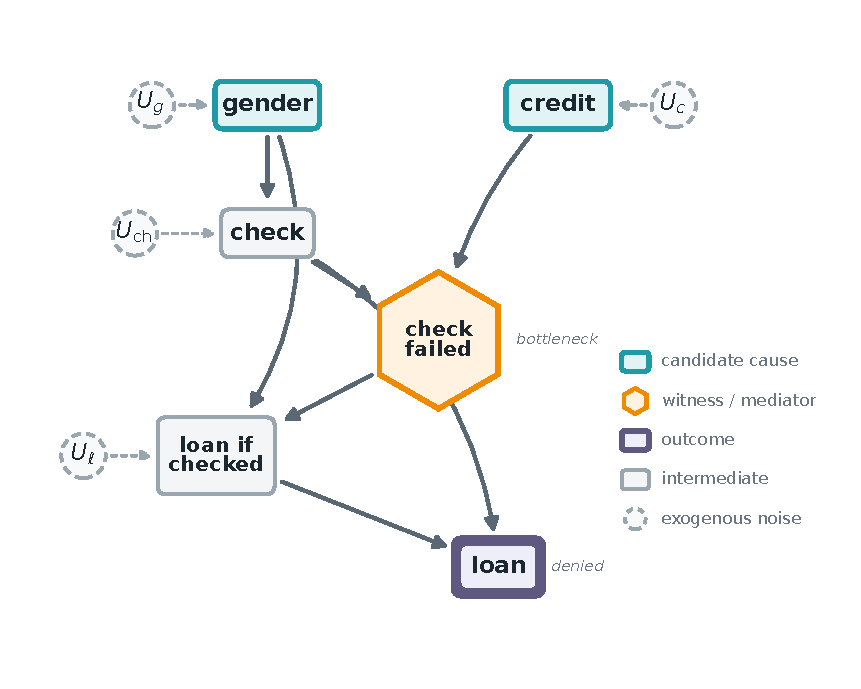
\includegraphics[width=0.62\linewidth]{figures/dag_obcb.pdf}
\caption[OBCB causal structure]{Causal structure of the OBCB loan model
(Example~\ref{ex:obcb_stochastic}). Node shape and colour encode role: the
\emph{candidate causes} \varname{gender} and \varname{credit} (teal boxes), the
\emph{witness} \varname{check-failed} (gold hexagon), and the \emph{outcome}
\varname{loan} (purple double box); intermediate variables are grey. Dashed circles
are the exogenous noise $U_V$ feeding each \emph{stochastic} mechanism---the
deterministic nodes \varname{check-failed} and \varname{loan} carry none. Note that
\varname{check} reaches \varname{loan} along two routes: through the
\varname{check-failed} bottleneck and directly as the screening gate
($\varname{loan}=\varname{loan-if-checked}\cdot\varname{check}$). \ourapproach holds
the bottleneck witness fixed to keep these two routes distinct.}
\label{fig:dag_obcb}
\end{figure}

\noindent The witness mechanism works well for deterministic models, but actual causality
in its standard form offers no straightforward way to handle probabilistic ones. Before
extending the witness idea to the stochastic setting, it is instructive to examine a
probabilistic approach that scales more naturally --- Pearl's probabilities of necessity
and sufficiency \citep{pearl2022probabilities} --- and to ask what it would miss without
witnesses. This will let us identify what probabilistic machinery is needed, and what
context-sensitivity is lost when witnesses are absent, motivating the synthesis that
\ourapproach provides.
The following definitions allow for probabilistic models, but assume that all variables are Boolean (PCI will relax this assumption,
 allowing for continuous variables).
Pearl considers two ways that a cause may relate to an effect: it may be necessary or sufficient for the effect.
A cause is necessary if, counterfactually absent the cause, the effect is unlikely to occur; it is sufficient
if the effect is counterfactually likely in the presence of the cause.
We now formalize these ideas and discuss them in the context of the running example.

\begin{definition}[Probability of Necessity]
Let the probability of necessity \citep{pearl1999probabilities} be the probability that the outcome $Y=y$ would not have occurred in the absence of  $C = c^\star$, given that both occurred: \[\pn(C = c^\star, Y = y^\star) = P\!\left(Y_{c'} \neq y^\star \;\middle|\; C = c^\star, Y = y^\star\right),\] where $Y_{c'}$ is the value of $Y$ after intervening on $C$ with $c'\neq c^\star$.\footnote{Read in twin-network fashion \citep{balke1994probabilistic, causalityPearl}: one draws an exogenous noise $\mathbf{u}\sim P_{\mathbf{U}}$, computes the factual $Y$ under the unintervened structural equations and the counterfactual $Y_{c'}$ under the intervened equations, and conditions on the joint event $\{C=c^\star,Y=y^\star\}$. Both $Y$ and $Y_{c'}$ live on the same probability space and share the same $\mathbf{u}$.}
\end{definition}

Strictly speaking, the probability of necessity is less specific to a particular situation than the actual-cause test above: as written, it conditions only on the cause--outcome pair, so it asks whether being male causes \emph{someone} to be denied, not whether it caused \emph{Bob} --- whose bad credit we already know --- to be denied.
We therefore report two readings.
The \emph{population-level} value conditions only on the cause and outcome, exactly as the definition prescribes.
The \emph{individual-level} value additionally conditions on the subject's other observed features (for Bob, on $\varname{credit}=\text{bad}$), specializing the query to that person.
The individual-level reading is the one closer to actual causation; we report both throughout, and the same population/individual split applies to $\ps$ and $\pns$ below.


We illustrate the computation for Alice's gender. Alice is factually
$\varname{gender}=\text{female}$, $\varname{credit}=\text{bad}$,
$\varname{loan}=F$; the counterfactual intervenes to set
$\varname{gender}=\text{male}$ while leaving $\varname{credit}=\text{bad}$.
Tracing the male-intervention branches through the model
(Appendix~\ref{app:obcb}, \S\ref{app:obcb_pn}) gives
$\pn(\varname{gender}=\text{female}, \varname{loan}=F \mid \text{Alice})
= 0.9 \cdot 0.05 = 0.045$.
Computing the analogous quantities for the remaining (variable, person) pairs gives
the individual-level values shown in Table~\ref{tab:pn_ps_pns}; the table also lists
population-level values for comparison.

The PN scores partially align with intuition: Bob's bad credit is high
($\pn=0.90$), and his gender score is zero, matching the reading that his gender played
no role.
But Alice's PN values do not separate gender (0.045) from credit (0.18)
particularly well, and Alice's gender PN is only marginally above Bob's, not the
sharp distinction we would want, given that the bank never even evaluated Alice's
credit.
PN cannot register this asymmetry: it asks counterfactually what would happen
under intervention without any context about which causal paths were active.
For the full picture we need a second quantity, the probability of sufficiency.

\begin{definition}[Probability of Sufficiency]
Let the probability of sufficiency be the probability that the outcome $Y=y^\star$ would have occurred in the presence of $C = c^\star$, given that neither $C=c^\star$ nor $Y=y^\star$ occurred:
\[\ps(C = c^{\star}, Y = y^\star) =  P\!(Y_{c^\star} = y^\star \;\vert\;  C = c',\ Y \neq y^\star)\]
where $c' \neq c^\star$ and $Y_{c^{\star}}$ is the value of $Y$ after intervening on $C$ with $c^\star$.
\end{definition}

To query whether the factual cause was sufficient, we condition on the counterfactual: we assume the cause did \emph{not} take its factual value and the outcome did \emph{not} occur, then intervene to restore the factual cause value and ask whether the outcome now occurs.
Intuitively, this asks: if the cause had been absent and things had gone differently, would reinstating the cause have brought the outcome about?
Let's look at the resulting values. 

We illustrate $\ps$ for Alice's gender. Following the same convention as for
$\pn$, the individual-level computation additionally conditions on Alice's
credit ($\varname{credit}=\text{bad}$): we fix her credit but flip the cause and
outcome to their non-factual values ($\varname{gender}=\text{male}$,
$\varname{loan}=T$), then intervene to restore $\varname{gender}=\text{female}$
and ask whether the loan is again denied. Both check branches yield
$\varname{loan}=F$ (Appendix~\ref{app:obcb}, \S\ref{app:obcb_ps}), so
$\ps(\varname{gender}=\text{female}, \varname{loan}=F \mid \text{Alice}) = 1$.
The remaining individual values, along with population-level values for comparison,
appear in Table~\ref{tab:pn_ps_pns}.
Two cases warrant comment: Bob's gender PS is undefined because the required
conditioning event ($\varname{gender}=\text{female}$, $\varname{credit}=\text{bad}$,
$\varname{loan}=T$) has probability zero in the model; Bob's credit PS is $0.955$
rather than $1$ because the model includes a $5\%$ exception rate for males who fail
the credit check.


To combine the insights of the two scores, we would like to find causes that are both necessary and sufficient.
This notion is  formalized as follows:

\begin{definition}[Probability of necessity and sufficiency]
Let the probability of necessity and sufficiency be the probability that the outcome $Y=y^\star$ would have occurred in the presence of $C = c^\star$ and that it would not have occurred under the intervention $C=c'$:
\[\pns(C = c^{\star}, Y = y^\star) =  P\!(Y_{c^{\star}} = y^\star, Y_{c'} \neq y^\star ).\]
This quantity factorises into a weighted sum of $\pn$ and $\ps$ by the
consistency rule of counterfactuals
\citep[\S 9.2]{causalityPearl}:
\[
  \begin{aligned}
    \pns(C = c^\star,\, Y = y^\star)
    &= P(C = c^\star,\, Y = y^\star)\,\pn(C = c^\star,\, Y = y^\star) \\
    &\quad + P(C = c',\, Y \neq y^\star)\,\ps(C = c^\star,\, Y = y^\star).
  \end{aligned}
\]
\end{definition}

\begin{table}[ht]
\centering
\small
\caption{$\pn$, $\ps$, and $\pns$ for Alice and Bob in
  Example~\ref{ex:obcb_stochastic}, with $\varname{loan}=F$ as the outcome.
  ``Population'' values condition only on the cause--outcome pair prescribed by the
  definition; ``Individual'' values additionally condition on the subject's other
  factual variable (e.g.\ for Alice's gender, on $\varname{credit}=\text{bad}$).
  A dash marks an entry that is undefined because the conditioning premises are
  inconsistent with the model.}
\label{tab:pn_ps_pns}
\vspace{4pt}
\begin{tabular}{ll @{\hspace{1.4em}} ccc @{\hspace{1.4em}} ccc}
\toprule
& & \multicolumn{3}{c}{Alice} & \multicolumn{3}{c}{Bob} \\
\cmidrule(lr){3-5}\cmidrule(lr){6-8}
Variable & Level & $\pn$ & $\ps$ & $\pns$ & $\pn$ & $\ps$ & $\pns$ \\
\midrule
$\varname{gender}$ & Population & 0.43  & 0.83 & 0.39  & 0.02  & 0.10  & 0.01 \\
$\varname{gender}$ & Individual & 0.045 & 1.00 & 0.045 & 0     & ---   & 0    \\[3pt]
$\varname{credit}$ & Population & 0.53  & 0.96 & 0.52  & 0.53  & 0.96  & 0.52 \\
$\varname{credit}$ & Individual & 0.18  & 1.00 & 0.18  & 0.90  & 0.955 & 0.86 \\
\bottomrule
\end{tabular}
\end{table}

The population- and individual-level $\pns$ values appear in the rightmost column
group of Table~\ref{tab:pn_ps_pns}.
These values capture the relative causal impact of $\varname{gender}$ and $\varname{credit}$ but are not entirely satisfying.
\Cref{tab:pn_ps_pns} reveals the problem directly: for Alice, $\pns(\varname{gender}) = 0.045 < \pns(\varname{credit}) = 0.18$, so PNS ranks credit as more causally responsible than gender.
Yet the bank never evaluated Alice's credit: the $\varname{check}$ variable was $F$ throughout.
PNS has no mechanism to register this: it asks counterfactually what would happen if credit were different, without fixing $\varname{check\text{-}failed}$, the mediating variable that blocked credit's causal path.

As an attempt to help us better understand Alice's particular situation, we might consider a modification of PNS with additional conditioning:
\[\pns_{c}(C = c^\star, Y = y^\star ~|~ Z=z^\star) = P(Y_{c^\star} = y^\star, Y_{c'} \neq y^\star ~|~ Z = z^\star)\]
Using this definition, we can compute $\pns_c(\varname{gender} = \text{female}, \varname{loan} = F ~|~ \varname{credit} = \text{bad}) = 0.045$ and $\pns_c(\varname{credit} = \text{bad}, \varname{loan} = F ~|~ \varname{gender} = \text{female}) = 0.18$.
Conditioning does not solve the problem described above (Alice's credit was in reality never evaluated) because the interventions override the mediating variable that tracks whether her credit has been checked.
When we compute $\pns_c(\varname{credit}=\text{bad}, \varname{loan}=F \mid \varname{gender}=\text{female})$, conditioning on gender being female is consistent with the factual, but when we then intervene to set credit to good, this intervention propagates downstream and changes $\varname{check\text{-}failed}$, overriding what we learned from conditioning on Alice's factual outcome.
The context we fixed is undone by the very intervention meant to probe it.
We will not consider this use of conditioning further, and this observation motivates the need to intervene on (as
opposed to condition) mediating variables that provide important context, which is what the witness mechanism provides.

\paragraph{ATE and CATE share the same limitation.}
The two most familiar causal quantities in the ML and policy literature are the average treatment effect
$\mathrm{ATE}(T) = \mathbb{E}[Y \mid do(T{=}1)] - \mathbb{E}[Y \mid do(T{=}0)]$
and the conditional version
$\mathrm{CATE}(T \mid X{=}x) = \mathbb{E}[Y \mid do(T{=}1), X{=}x] - \mathbb{E}[Y \mid do(T{=}0), X{=}x]$.
Computed on our stochastic OBCB, population ATE ranks credit ($0.518$) above gender ($0.383$),
mirroring the population PN ranking.
At the individual level for Alice, $\mathrm{CATE}(\varname{credit}\mid\varname{gender}{=}\text{female}) = 0.18$
and $\mathrm{CATE}(\varname{gender}\mid\varname{credit}{=}\text{bad}) = 0.045$.
These are exactly Alice's individual $\pns$ values: with binary outcomes and $\ps = 1$ in the
relevant branches, CATE for a single treatment collapses to $\pns_c$, so the same
$\varname{check\text{-}failed}$ propagation that undermined $\pns_c$ undermines CATE.
A second, sharper failure follows from CATE's inability to condition on the factual
treatment value: $\mathrm{CATE}(\varname{gender}\mid\varname{credit}{=}\text{bad}) = 0.045$ is identical
for Alice and Bob even though one's gender carried her denial outright while the other's
merely opened the credit check that then rejected him.
The structural limitation cuts across PNS, ATE, and CATE alike,
which is why the witness mechanism in Section~\ref{sec:causal_impact} is not
just a fix for PNS but a general repair for the family of methods that average
counterfactual effects without intervention-based context-sensitivity.



\subsection{Path Forward}

The two predecessors examined in this section have complementary strengths and blind spots.
Halpern's actual causality is context-sensitive: by holding witnesses fixed at their factual values, it correctly diagnoses Alice's case, attributing her denial to gender rather than credit.
But in its standard form it is restricted to deterministic models, it requires a brute-force search over witness sets, and it has no native treatment of continuous variables.
Pearl's PN/PS/PNS make the converse trade-off.
They scale naturally to probabilistic models, because every counterfactual reduces to an expectation under the noise distribution.
But they have no analogue of the witness mechanism: every intervention propagates through the structural equations and overrides whatever mediator value the factual context fixed.
Table~\ref{tab:pn_ps_pns} shows the symptom: for Alice, $\pns(\varname{credit}) > \pns(\varname{gender})$, even though the credit check was never performed.

Any replacement therefore needs intervention-based context-sensitivity, holding the relevant mediators fixed by intervention.
\ourapproach{} delivers exactly this, combining three ingredients into a single estimator.
From actual causality it takes the \emph{witness mechanism}: it holds relevant context fixed by intervention, so the structural information about which causal paths were active survives the counterfactual evaluation.
From PN/PS/PNS it takes a \emph{probabilistic vocabulary}: it expresses counterfactuals as expectations under the noise distribution, so the attribution lives on the same probability space as the model and extends naturally to continuous variables.
And in place of brute-force enumeration over witness sets, it \emph{integrates} over a distribution of them --- an integral estimable from samples even when the witness pool is large or the variables continuous.

Returning to Alice, \ourapproach{} recovers the intuitive verdict that her denial turns on gender rather than credit --- reversing the ranking $\pns$ produced (Table~\ref{tab:pn_ps_pns}).
We revisit the example in full once the method is defined (Section~\ref{sec:causal_impact}, with the complete computation in Appendix~\ref{app:obcb}).

Two features distinguish \ourapproach{} from both predecessors.
Unlike actual causality, it does not ask whether \emph{some} witness set validates a counterfactual dependency; it integrates over a distribution of witness sets, weighting each by its probability.
This replaces combinatorial enumeration with statistical estimation.
The gain is also conceptual. Existential quantification certifies a cause as soon as \emph{some} witness set validates the dependence, a sensitivity that graded and normality-based accounts were introduced in part to address; integration instead weights each witness set by its probability, so a variable is responsible to the degree that \emph{typical} contexts render it efficacious.
The witness still does the essential work of holding context fixed --- \ourapproach{} simply declines to privilege one hand-picked set, letting the structural facts decide which witnesses carry the mass (for Alice, those pinning $\varname{check\text{-}failed}$ favour gender; almost none favour credit).
As a by-product, actual causality's binary verdict becomes a graded magnitude.
Unlike PN/PS/PNS, it inherits the context-sensitivity of actual causality through this integration: causally inert variables are downweighted automatically, because almost every witness set leaves them disconnected from the outcome, while variables that drive the outcome are upweighted, because almost every witness set leaves them connected.
The formal definitions in Section~\ref{sec:causal_impact} make this expectation precise.

\medskip\noindent With the limitations of both predecessors in mind, we turn
in Section~\ref{sec:causal_impact} to the formal development. The next section
introduces \ourapproach piece by piece --- PSCM scaffolding, the variable
selection distribution $\Gamma$, the alternative-value distribution $\Delta$, the
joint necessity-sufficiency measure, and the user-chosen causal impact function
$ci$ --- and verifies on the same Alice/Bob example that the resulting attribution
satisfies all seven desiderata stated at the start of that section.





\section{Causal Impact: Definitions}\label{sec:causal_impact}

Explanation and causal attribution seek to connect a potentially causal \textit{event} $X=x$ to an outcome event $Y=y$.\footnote{This is quite different from type-level causal queries, where one is interested in some group-level attribution, as when one estimates average treatment effect or conditional average treatment effect.}
% To measure the strength of causation, we (i) intervene to change $X$ and measure the extent to which this changes $Y$ (call this a \emph{necessity intervention}), and (ii) intervene on $X$ to have the actual value and measure the extent to which this ensures $Y=y$ (call this a \emph{sufficiency intervention}), while (iii) preserving context-sensitivity, and (iv) allowing for some variation in which parts of the contexts are fixed and in what combinations the cause candidates are intervened on, to account for interactions.
% Moreover, (v) to search for causes, we also need to perform a search through potential sets of causes.
In this section, we present a formal development. To ground it, we return to Example~\ref{ex:obcb_stochastic} and
 use Alice and Bob as running illustrations throughout this section. Both are rejected for a loan; the question is
 which of their attributes (\varname{gender} and \varname{credit}) was causally responsible for each rejection,
 and to what degree. While the example is discrete, the machinery applies to continuous and mixed-type variables;
  a continuous illustration is given in Sections~\ref{sec:signal} and~\ref{sub:synthetic}.

\paragraph{Roadmap of this section.}
We state seven \emph{desiderata} that any responsibility attribution for Alice and Bob should satisfy, giving the formal construction an explicit target. We introduce the probabilistic
structural causal model (PSCM) and interventions, the substrate on which everything
else rests, and then the two distributions \ourapproach offers to the user: the
variable selection distribution $\Gamma$ over suspect/witness pairs and the
alternative-value distribution $\Delta$ over counterfactual cause settings. We combine
these into the joint necessity-sufficiency measure $P_k^{s,n}$ and the user-chosen
causal impact function $ci$ whose expectation is the \ourapproach score, showing how
the choice of $ci$ generalises the framework from binary to continuous outcomes.
Finally we compute the score on the OBCB example, verify that all seven desiderata
hold, and contrast \ourapproach's necessity/sufficiency decomposition with Pearl's
PN/PS/PNS.

Let $R(V \rightsquigarrow \varname{loan} \mid \text{person})$ denote the causal responsibility of variable $V$
for the loan outcome at the individual level ($R$ is a placeholder for any attribution score and
should not be identified with a specific formal quantity; \ourapproach interprets $R$ as the
PCI score $\mathrm{PCI}_{X_k}$ of Definition~\ref{def:causalimpact}, but the desiderata are
method-agnostic). Here $V$ ranges over the candidate variables; in the general development
it is the variable of interest $X_k$.
Attribution methods may produce signed values; the desiderata are stated in terms of absolute
magnitudes $|R(\cdot)|$, allowing for directionality:
\label{desid}
\begin{align*}
\textbf{D-A1} \quad & |R(\varname{gender} \rightsquigarrow \varname{loan} \mid \text{Alice})| > 0 \\[2pt]
\textbf{D-A2} \quad & |R(\varname{credit} \rightsquigarrow \varname{loan} \mid \text{Alice})| > 0 \\[2pt]
\textbf{D-A-rank} \quad & |R(\varname{gender} \rightsquigarrow \varname{loan} \mid \text{Alice})| > |R(\varname{credit} \rightsquigarrow \varname{loan} \mid \text{Alice})| \\[6pt]
\textbf{D-B1} \quad & |R(\varname{gender} \rightsquigarrow \varname{loan} \mid \text{Bob})| > 0 \\[2pt]
\textbf{D-B2} \quad & |R(\varname{credit} \rightsquigarrow \varname{loan} \mid \text{Bob})| > 0 \\[2pt]
\textbf{D-B-rank} \quad & |R(\varname{credit} \rightsquigarrow \varname{loan} \mid \text{Bob})| > |R(\varname{gender} \rightsquigarrow \varname{loan} \mid \text{Bob})| \\[6pt]
\textbf{D-comp} \quad & |R(\varname{gender} \rightsquigarrow \varname{loan} \mid \text{Alice})| > |R(\varname{gender} \rightsquigarrow \varname{loan} \mid \text{Bob})|
\end{align*}

\noindent \textbf{D-A1} and \textbf{D-A2} both require non-zero attribution for Alice because two
distinct causal routes were available. Gender filtered her out at the checking stage. Credit is not
causally inert either: the check is only \emph{probabilistic} (women are still checked with positive
probability, $\gamma_F=0.2$ in the model below), so conditioning on Alice's denial leaves nonzero
probability that she was in fact checked, in which case her bad credit was the operative cause. The
broader principle is a graded ordering of three roles. An \emph{active} cause, on the path that actually
produced the outcome, carries the most responsibility. A \emph{preempted} cause is not discarded but
retains a \emph{residual} share, strictly positive yet strictly below the active cause (exactly what
\textbf{D-A-rank} demands), here governed by the probability that the preemption fails to fire,
leaving the credit route live. An \emph{irrelevant} variable, with no active path to the outcome under
any context, receives the least of all, approaching zero. This is a deliberate departure from the binary
Halpern--Pearl/Beckers treatment of preemption, which collapses the first two roles by zeroing a fully
preempted cause. \textbf{D-A-rank} is the substantive constraint: because Alice never underwent a
credit evaluation, gender's causal role is immediate, whereas credit's is purely
hypothetical. A method that ranks credit above gender for Alice is misattributing the cause of her
rejection.

For Bob, \textbf{D-B2} reflects that the credit check occurred and directly produced the rejection:
the causal chain $\varname{credit} \to \varname{check\text{-}failed} \to \varname{loan}$ was
activated. \textbf{D-B1} requires strictly positive attribution for \varname{gender}: being male
gave Bob a $90\%$ probability of being checked, so gender opened the evaluation that rejected him.
This indirect causal role is non-zero; a method returning exactly zero fails to capture it.
\textbf{D-B-rank} corresponds to the intuition that credit is the proximate cause.
\textbf{D-comp} captures the cross-individual asymmetry that is hardest for naive methods to
express: gender is more causally responsible for Alice's rejection than for Bob's, because for
Alice \varname{gender}=female was sufficient on its own to produce the rejection (no
evaluation took place, so credit was never a factor), while for Bob \varname{gender}=male
merely opened the evaluation that \varname{credit}=bad then caused.
We will verify at the end of this section that \ourapproach satisfies all seven desiderata,
while PN, PS, PNS fail some of them. Later, we will also revisit this example and its
 desiderata in the context of SHAP and Causal SHAP (Section~\ref{sec:shap_examples}).

We work within the context of probabilistic structural causal models \citep{causalityPearl}.
\begin{definition}[Probabilistic Structural Causal Model (PSCM)]
A probabilistic structural causal model is a tuple
\[
M = \langle \mathbf{U}, \mathbf{V}, \mathbf{F}, P_{\mathbf{U}} \rangle,
\]
where \(\mathbf{V} = \{V_1,\dots,V_n\}\) is a finite set of endogenous variables,
\(\mathbf{U} = \{U_1,\dots,U_n\}\) is a set of exogenous variables,
and \(\mathbf{F} = \{f_1,\dots,f_n\}\) is a set of structural assignments
\[
V_i := f_i(\mathbf{Pa}_i, U_i), \qquad i = 1,\dots,n,
\]
with \(\mathbf{Pa}_i \subseteq \mathbf{V}\setminus\{V_i\}\) denoting the parents of \(V_i\).
The distribution \(P_{\mathbf{U}}\) is a probability measure on $\dom(\mathbf{U})$,
and the assignments in \(\mathbf{F}\) are assumed to be acyclic and to have a unique solution for \(\mathbf{V}\) given \(\mathbf{U}\).\footnote{Working within the PSCM framework commits the practitioner to fully specified structural assignments $\mathbf{F}$ and an exogenous distribution $P_{\mathbf{U}}$, analogous to how Bayesian inference requires a likelihood and a prior. This is precisely what enables \ourapproach to yield individual-level counterfactual attributions rather than population-level bounds, and once $\mathbf{F}$ and $P_{\mathbf{U}}$ are specified, sampling from $P_{\mathbf{U}}$ is a routine probabilistic inference operation.}
\end{definition}

\medskip\noindent A PSCM encodes which variables influence which others, 
through what mechanisms, and subject to what randomness. The structural equations specify
 each variable as a deterministic function of its causal parents and local noise; the exogenous 
 distribution captures all irreducible uncertainty in the system. Together they make every counterfactual
  question well-posed and computable.


The OBCB model (Example~\ref{ex:obcb_stochastic}) is a PSCM with endogenous
variables
\[
\mathbf{V}=\{\varname{gender},\varname{credit},\varname{check},\varname{check\text{-}failed},\varname{loan\text{-}if\text{-}checked},\varname{loan}\},
\]
and exogenous variables
\[
\mathbf{U}=\{U_{\varname{gender}},U_{\varname{credit}},U_{\varname{check}},U_{\varname{loan\text{-}if\text{-}checked}}\}
\]
which induce independent Bernoulli noise.

The structural assignments in the case at hand take the form $V_i = f_i(\mathbf{Pa}_i, U_i)$
promised by the PSCM definition above. Each stochastic node is a Bernoulli draw whose
success probability is a primitive parameter of the model (possibly depending on the
node's parents); writing $V \sim \mathrm{Bernoulli}(p)$ for a node equal to $1$ with
probability $p$, the mechanisms are
\begin{align*}
\varname{gender}        &\sim \mathrm{Bernoulli}(p_g), \\
\varname{credit}        &\sim \mathrm{Bernoulli}(p_c), \\
\varname{check} \mid \varname{gender}        &\sim \mathrm{Bernoulli}\bigl(\gamma_F(1-\varname{gender}) + \gamma_M\,\varname{gender}\bigr), \\
\varname{check\text{-}failed}  &= \varname{check}\,(1-\varname{credit}), \\
\varname{loan\text{-}if\text{-}checked} \mid \varname{gender}, \varname{check\text{-}failed} &\sim \mathrm{Bernoulli}\bigl(\mathrm{loan\text{-}prob}(\varname{gender}, \varname{check\text{-}failed})\bigr), \\
\varname{loan}          &= \varname{loan\text{-}if\text{-}checked} \cdot \varname{check}.
\end{align*}
So \varname{gender} and \varname{credit} are fair coin flips; \varname{check} fires with
probability $\gamma_F$ for women and $\gamma_M$ for men; \varname{check\text{-}failed} and
\varname{loan} are deterministic functions of the nodes above them
(Figure~\ref{fig:dag_obcb}). The Bernoulli draws are coupled across factual and counterfactual worlds, making counterfactuals well-defined. For the running example we take $p_g = p_c = 0.5$,
$\gamma_F = 0.2$, $\gamma_M = 0.9$, and the values of $\mathrm{loan\text{-}prob}$
given in Example~\ref{ex:obcb_stochastic}.

\begin{definition}[Interventions]
Given a model \(M = \langle \mathbf{U}, \mathbf{V}, \mathbf{F}, P_{\mathbf{U}} \rangle\),
an intervention on variables \(\mathbf{X} = \{X_1, \dots, X_k\} \subseteq \mathbf{V}\)
with values \(\mathbf{x} = (x_1, \dots, x_k)\) replaces the structural assignments for \(X_i\) by $X_i := x_i$, where $i = 1, \dots, k$.
We denote this intervention by either \([\mathbf{X} \leftarrow \mathbf{x}]\) or $do(\mathbf{X} = \mathbf{x})$.
\end{definition}

\medskip\noindent An intervention surgically replaces a variable's structural equation with a fixed constant, 
disconnecting it from its usual causes. The rest of the model propagates downstream as normal under the new assignment;
 the exogenous noise is unchanged.

In the OBCB model, $\mathrm{do}(\varname{gender}=1)$ replaces Alice's gender assignment with male, leaving all other structural equations intact. The downstream effect propagates: \varname{check} now draws from $\mathrm{Bern}(0.9)$ rather than $\mathrm{Bern}(0.2)$, so Alice would be checked in 90\% of noise realizations instead of 20\%. This is the counterfactual world in which we ask whether her loan outcome would have differed.

Because \ourapproach supports arbitrary variable types, it will be helpful to define a measure theoretic object corresponding to interventional outcomes. Because outcomes are a deterministic function of exogenous noise, this will be a Dirac measure.

\begin{definition}[Pointwise Interventional Law] \label{def:interlaw}
Let $M=\langle \mathbf{U},\mathbf{V},\mathbf{F},P_{\mathbf{U}}\rangle$ be a probabilistic
structural causal model and let $Y\in\mathbf{V}$.
For an intervention $\mathrm{do}(\mathbf{X}=\mathbf{x})$, let
$Y':\dom(\mathbf{U})\to\dom(Y)$ denote the measurable map induced by the
modified structural assignments.
The \emph{pointwise interventional law} of $Y$ at fixed $\mathbf{u}\in\dom(\mathbf{U})$ is the probability measure on
$\dom(Y)$ defined by
\[
P\!\left(Y\in A \mid \mathbf{u},\mathrm{do}(\mathbf{X}=\mathbf{x})\right)
\;:=\;
\mathbb{I}\!\left\{Y'(\mathbf{u})\in A\right\}
\;=\;\delta_{Y'(\mathbf{u})}(A),
\qquad
A\subseteq\dom(Y).
\]
\end{definition}

\medskip\noindent The pointwise interventional law records the deterministic
outcome of $Y$ under $\mathrm{do}(\mathbf{X}=\mathbf{x})$ for a fixed noise realization
$\mathbf{u}$: since the modified structural equations make $Y$ a function of $\mathbf{u}$
alone, its distribution collapses to a point mass. Integrating over $P_{\mathbf{U}}$
then recovers the full interventional distribution.

We define a \emph{causal set} to be a set of assignments to the variables of a probabilistic structural causal model.

\begin{definition}[Causal set]
Given a model \(\langle \mathbf{U}, \mathbf{V}, \mathbf{F}, P_{\mathbf{U}}\rangle\), a causal set is a set of pairs $X = x$ where $X \in \mathbf{V}$ and $x \in \mathit{dom}(X)$.
\end{definition}

\medskip\noindent Informally, a causal set is a list of specific variable-value
assignments, a precise statement of which variables are set to which values. It is the
basic unit of intervention: from a causal set one can read off exactly what is being
manipulated or held fixed.

In \ourapproach, causal sets play four distinct roles, two on the cause side and two
on the context side:

\begin{description}
\item[Suspects $\mathbf{S}$.] The full set of variables suspected to bear on the
outcome. Subsets of $\mathbf{S}$ will be sampled and intervened on.
\item[Active suspects $\mathbf{C} \subseteq \mathbf{S}$.] The specific subset
intervened on in a given search step, either to alternative values (necessity
regime) or to factual values (sufficiency regime).
\item[Witnesses $\mathbf{W}$.] The full set of context variables that may be held fixed
at their factual values. Subsets of $\mathbf{W}$ will be sampled and held fixed.
\item[Active witnesses $\mathbf{T} \subseteq \mathbf{W}$.] The specific subset held
fixed in a given search step. To avoid contradicting the active intervention,
$\mathbf{T}$ is pruned so that $\mathbf{T} \cap \mathbf{C} = \emptyset$.
\end{description}

\medskip\noindent
\textbf{Why prune $\mathbf{T}$ and not $\mathbf{C}$?}
The conflict on $\mathbf{T} \cap \mathbf{C}$ has to be resolved in one
direction or the other, and pruning the witnesses is the right choice for
three reasons.
First, $\mathbf{C}$ is the object of the test: it encodes the causal claim
being evaluated, while $\mathbf{T}$ is the auxiliary device that holds
context fixed.
Pruning $\mathbf{C}$ would silently change the claim under test; pruning
$\mathbf{T}$ leaves the claim intact and merely weakens the context held fixed.
Second, the convention extends cleanly to the limit $\mathbf{C} = \mathbf{V}$,
where every variable is a suspect: the pruned $\mathbf{T}$ collapses to
$\emptyset$ and we recover the unconditional but-for test, the right
baseline behaviour.
Pruning $\mathbf{C}$ instead would leave this limit undefined whenever any
witness is sampled.
Third, the convention inherits directly from Halpern's actual-cause
definition (Definition~\ref{def:ac_intuitive}), which makes
$\mathbf{T} \cap \mathbf{C} = \emptyset$ part of the definition;
pruning post-sampling is the operational implementation of that constraint
and lets us specify $\Gamma$ on the unconstrained product
$2^{\mathbf{S}} \times 2^{\mathbf{W}}$ rather than baking disjointness into
the prior.

To evaluate the causal impact of a variable on an outcome, we consider two interventional regimes: the \emph{necessity regime}, 
in which we intervene on the variables $\mathbf{C} \subseteq \mathbf{S}$ to have an alternative value, and the sufficiency regime,
 in which we intervene so that $\mathbf{C}$ takes on factual values. 
Moreover, we hold some elements $\mathbf{T} \subseteq \mathbf{W}$ of the context fixed (i.e., intervened on to retain factual values, despite intervention on $\mathbf{C}$). This is exactly what makes the necessity component \emph{context-sensitive} in Halpern's sense \citep{actualCausalityHalpern}: the alternative cause is evaluated against a held-fixed witness configuration, not in isolation. We will reuse this terminology throughout: ``context-sensitive necessity'' refers to the necessity regime evaluated under an active witness set $\mathbf{T}$.
When looking for an explanation, we perform a search across possible cause sets and possible contexts.
Complete model samples in these regimes will be called \emph{necessity worlds}  and \emph{sufficiency worlds}, respectively.

The intuition is that 
the suspect set $\mathbf{S}$ names every variable that could plausibly have caused the outcome; the witness set $\mathbf{W}$ names context
variables to be selectively held fixed, isolating the causal channels under investigation. Intervening
on suspects tests what would have happened under an alternative cause in the necessity worlds and under the factual values
 in the sufficiency worlds; fixing witnesses
blocks confounding paths that would otherwise absorb the effect.
Responsibility attribution increases when the outcome is far from the factual value in the necessity world and decreases 
when it is far from the factual value in the sufficiency world.




For both Alice (female, bad credit, loan denied) and Bob (male, bad credit, loan denied)
we set $\mathbf{S} = \{\varname{gender}, \varname{credit}\}$ and
$\mathbf{W} = \{\varname{check\text{-}failed}\}$. The witness \varname{check\text{-}failed}
records whether the applicant was checked and had bad credit; holding it at its factual
value isolates the causal path from \varname{gender} or \varname{credit} to \varname{loan}
independently of the credit-check bottleneck. Without this witness, intervening on
\varname{credit} for Alice would leave 80\% of noise realizations unaffected (those
in which she is never checked), making credit's causal role invisible. The witness makes
the bottleneck explicit and manipulable.

In the general framework we search for causes by intervening on subsets of suspects
and holding fixed subsets of witnesses. To make this search tractable, we need a way to prioritize which subsets to consider.

\begin{definition}[Variable Selection Distribution]
Let $\mathbf{X}$ be a finite set of random variables. A \emph{variable selection distribution} $\Gamma$ is a probability distribution on $2^\mathbf{X}$. We write $\mathbf{Y}\sim\Gamma$ to mean $\mathbf{Y}$ is a random subset of $\mathbf{X}$ drawn from $\Gamma$, with $p^\Gamma(\mathbf{y})$ denoting the probability assigned to $\mathbf{y}\subseteq\mathbf{X}$.
\end{definition}

\medskip\noindent The variable selection distribution $\Gamma$ encodes
prior beliefs about which subsets of suspects are worth examining. A uniform distribution
treats all suspect subsets as equally plausible; a cardinality-constrained choice focuses
the search on interactions of a particular order, analogous to choosing which interaction
terms to include in a regression. More complex distributions could encode domain knowledge
about which variables are more likely to interact, or could be learned from data.

\noindent In particular, we will be using variable selection distributions for the powerset of causal suspects $\mathbf{S}$ and for the powerset of witnesses $\mathbf{W}$. One simple pattern of suspect and witness selection can be derived by setting size limits on the number of activated suspects or witnesses, and sampling uniformly otherwise.

\begin{example}[Cardinality-Constrained Uniform Selection]
Let $\mathbf{X}$ be a candidate set of random variables and let $k \sim \mathrm{Unif}\{J, \dots K\}$ with $1 \leq J \leq K \leq |\mathbf{X}|$. A variable selection $\mathbf{Y} \sim \Gamma(2^\mathbf{X})$ is sampled from a cardinality-constrained uniform selection distribution $\Gamma(2^\mathbf{X})$ with probability mass function
\[
p^\Gamma(\mathbf{Y}) \propto \mathbb{I}[|\mathbf{Y}| = k].
\]

The parameters $J$ and $K$ determine the cardinality range of the search; specific
choices connect \ourapproach to existing methods and enable efficient Monte Carlo
approximation.\footnote{When $J=1$ and $K=|\mathbf{X}|$, this distribution coincides with the Shapley weighting kernel, which samples coalition size uniformly and then selects a coalition uniformly at that size \citep{shapley1953}. The parameters $J$ and $K$ allow the practitioner to restrict the search to cause sets of a specific cardinality range: setting $J=K=1$ confines attribution to individual variables, while $J=2, K=3$ focuses on small multi-variable interactions. Moreover, whereas exact Shapley computation requires summing over all $2^{|\mathbf{X}|}$ coalitions, \ourapproach treats $\Gamma$ as a generative model: approximation proceeds by sampling subsets from $\Gamma$ and outcomes from $P_{\mathbf{U}}$, making Monte Carlo estimation a native feature of the framework rather than an external
algorithmic layer.
We note that the weighting alone does not distinguish PCI from SHAP at $J=1$,
$K=|\mathbf{X}|$: the subset weights are identical. The distinction lies in the
integrand, and it matters for what is being evaluated and what results follow. SHAP
averages marginal contributions using the observational conditional
$\mathbb{E}[f(\mathbf{X}_{\mathcal{S}} = \mathbf{x}_{\mathcal{S}}, \mathbf{X}_{\bar{\mathcal{S}}})]$, marginalising over
the empirical distribution of non-suspect features; this means a variable that is merely
correlated with a cause, but not itself causally active, can receive positive
attribution. \citet{janzing2020feature} frame exactly this as a causal problem,
arguing that dropping a feature should be \emph{interventional} rather than
observational, since the conditional version lets a feature inherit relevance from its
correlates. PCI instead evaluates counterfactual outcomes
$P(Y \in A \mid \mathbf{u},\, \mathrm{do}(\mathbf{C}=\mathbf{c}',
\mathbf{T}=\mathbf{t}^\star))$ computed via the structural model, so attribution flows
only along genuine causal paths. The witness mechanism adds a further distinction: by
holding intermediate variables fixed, PCI can resolve overdetermination and undercutting
scenarios where SHAP assigns equal or incorrect attribution. The choice of $J$ and $K$
remains a design decision; practitioners can set $J=K=1$ for single-variable attribution
or allow higher-order interactions as discussed above. A detailed comparison of PCI,
SHAP, and Causal SHAP on concrete examples is given in
Section~\ref{sec:shap_examples}.}
\end{example}

In \ourapproach the variable selection distribution $\Gamma$ is a probability
mass function on $2^{\mathbf{S}} \times 2^{\mathbf{W}}$, governing the joint
choice of an active suspect set $\mathbf{C} \subseteq \mathbf{S}$ and an active
witness set $\mathbf{T} \subseteq \mathbf{W}$. The recommended construction
samples suspects and witnesses separately and then enforces the constraint
that no variable plays both roles in the same draw: pick a marginal $\Gamma_s$
on $2^{\mathbf{S}}$ and a marginal $\Gamma_w$ on $2^{\mathbf{W}}$, draw
$\mathbf{C}\sim\Gamma_s$ and $\mathbf{T}\sim\Gamma_w$ independently, and
\emph{reject} any draw with $\mathbf{T}\cap\mathbf{C}\neq\emptyset$,
resampling until the constraint holds. Equivalently,
\[
p^\Gamma(\mathbf{C}, \mathbf{T}) \;\propto\;
p_s^\Gamma(\mathbf{C})\,p_w^\Gamma(\mathbf{T})\,
\mathbb{I}[\mathbf{T}\cap\mathbf{C}=\emptyset].
\]
 Throughout, $\Gamma_s$ and $\Gamma_w$ are
abbreviations for the sampling marginals of this construction; the formal
primitive in Definition~\ref{def:jointnecsuf} is the joint $\Gamma$.

For the OBCB analysis, with $|\mathbf{S}|=2$, we use a $\Gamma$ built from
$\Gamma_s$ uniform over the three non-empty subsets of $\mathbf{S}$
($\{\varname{gender}\}$, $\{\varname{credit}\}$,
$\{\varname{gender}, \varname{credit}\}$, each with probability $1/3$) and
$\Gamma_w$ uniform over $\{\emptyset, \{\varname{check\text{-}failed}\}\}$,
each with probability $1/2$. Since no element appears in both $\mathbf{S}$
and $\mathbf{W}$, the rejection step is vacuous and $\Gamma$ is exactly the product of marginals $p_s^\Gamma\cdot p_w^\Gamma$. In larger suspect sets the choice of cardinality
range becomes substantive: sampling uniformly from the full powerset yields an
expected intervention size of $|\mathbf{S}|/2$, which spreads attribution
across large coalitions and may make individual feature contributions harder
to isolate; we return to this issue in \cref{sec:ac_benchmark}, where
the cardinality cap is treated as a tunable hyperparameter and a
dynamic-set-sizes ablation measures the empirical cost of bounding it.

The choice of $\Gamma$ is a design decision that shapes the search process and the
resulting attributions.
As a default, a uniform $\Gamma$ over the full powerset is the least-informative
starting point, assigning equal weight to all subset sizes, analogous to including all
interaction orders in a regression. There is no universally principled criterion for
restricting the cardinality range; we therefore recommend treating $J$ and $K$ as
explicit design choices. Two practical considerations bear on this choice, however: with $K=1$, attribution
scores are based on singleton interventions and straightforward to communicate to
stakeholders; higher $K$ averages over joint interventions on $X_k$ with other suspects
simultaneously, which is harder to explain and, in large or structurally complex models,
may amplify estimation noise rather than capturing genuine higher-order causal structure.
For applications where attribution has serious consequences, we recommend a
cardinality sensitivity analysis: if rankings are stable as $K$ increases from $1$ to
$|\mathbf{S}|$, the simpler choice is supported; if they diverge, higher-order
interactions are materially relevant and the full powerset should be used. The key
advantage of \ourapproach is that this commitment is made transparently rather than
absorbed into an implicit default.\footnote{SHAP faces an analogous decision without
flagging it as one: by averaging over all $2^{|N|}$ feature coalitions, plain SHAP and
Causal SHAP commit to the maximum interaction order $K=|N|$ as an unstated default,
with no diagnostic offered for whether that level of joint conditioning is right for a
given model. Restricting SHAP to $K<|N|$ would break the efficiency axiom, so the
choice is hardcoded into the framework rather than treated as a tunable. \ourapproach{}
makes the same decision an explicit choice.}

Causal attribution hinges on questions such as ``if $X$ had, contrary to fact, been fixed to $x'\ne x$ instead of $x$, what would the outcome have been?'' For non-binary causes, this is ambiguous. To resolve this in a way that does not require committing to a single, contrastive causal event \citep{kawakammi_2024_poc_for_cont_and_vec}, we rely on a \textit{distribution} over alternative values.

% \begin{definition}[Alternative Value Distribution]
% Consider a set of random variables $\mathbf{X}$ and event $\mathbf{X}=\mathbf{x}\in dom(\mathbf{X})$. An alternative value $\mathbf{x}' \sim \Delta(\mathbf{x})$ is sampled from the alternative value distribution $\Delta(\mathbf{x})$, where $\mathbf{x}' \in dom (\mathbf{X})$ and $p_\Delta(\mathbf{x}') = \mathbb{P}(\mathbf{X}'=\mathbf{x'})$ with $dom(\mathbf{X}) = dom(\mathbf{X}')$.
% \end{definition}

\begin{definition}[Alternative Value Distribution]
Let $\mathbf{X}$ be a set of random variables with domain $\dom(\mathbf{X})$ and
let $\mathbf{X}=\mathbf{x}\in\dom(\mathbf{X})$ be a factual event.
An \emph{alternative value distribution} $\Delta(\mathbf{x})$ is a probability
measure on $\dom(\mathbf{X})$ such that $\mathbf{x} \notin \operatorname{supp}(\Delta(\mathbf{x}))$.
\end{definition}

\medskip\noindent Informally, $\Delta(\mathbf{x})$ specifies what counts as a
genuinely different value for a suspect variable. The support condition ensures no mass
falls on the factual value $\mathbf{x}$ itself, so every sampled alternative is a real
counterfactual departure rather than a noisy copy of what actually happened.

\medskip\noindent Three properties guide the choice of $\Delta$.
\emph{Plausibility under $M$:} the alternative should be a value the structural model
could plausibly produce given the context, so the necessity test interrogates a
counterfactual the model has anything to say about.
\emph{Outcome-independence:} the distribution over $\mathbf{x}'$ should not be informed
by the outcome whose causes we are explaining, on pain of circularity.
\emph{Context-sensitivity:} $\mathbf{x}'$ should reflect the rest of the factual
scenario, so the necessity test is individual-level rather than population-level.
The construction we use throughout is the structural-model posterior of $\mathbf{X}$
conditioned on upstream factual values, optionally excised near the factual value
(Example~\ref{ex:eps_excised} below); this is the natural choice satisfying all three.

\medskip\noindent Upstream-only conditioning operationalises the intuition shared with
the descriptive-normality literature \citep{Halpern2015-HALGCA,
icardNormalityActualCausal2017, hitchcock2009cause}: factual upstream values play the role of the
\emph{default} against which counterfactual alternatives are graded, the same role a
stipulated baseline plays in causal analyses of harm \citep{beckersHarm2022}, where a
default contract fixes what counts as a departure from the expected course of events.
\ourapproach does not aim to resolve the specific counterexamples motivating that
literature; the link is at the level of \emph{why} a non-uniform $\Delta$ matters at
all.
Since $\Delta$ is user-pluggable, other constructions are available when domain
knowledge motivates them: a uniform distribution over $\dom(\mathbf{X})$ trades
plausibility for breadth; the empirical marginal $p(\mathbf{x}')$ trades
context-sensitivity for simplicity; a fully conditional posterior on every observable
(including downstream evidence) trades outcome-independence for sharper conditioning.


\noindent One natural alternative value distribution results from taking the one currently embodied in the model and excising it around the factual setting. Then, the semantics for  ``alternative value'' means ``a sufficiently different value, following the original distribution otherwise''. In the discrete case, of course, the analogue is simply the probability mass function conditioned on the factual value not holding.



\begin{example}[$\epsilon$-Excised Distribution]\label{ex:eps_excised}
Assume $\mathbf{X}$ is $\mathbb{R}^d$-valued with density $p$.
Given a factual event $\mathbf{X}=\mathbf{x}$, define the
$\epsilon$-excised alternative value distribution $\Delta_\epsilon(\mathbf{x})$
as the probability measure on $(\mathbb{R}^d,\mathcal{B}(\mathbb{R}^d))$ with density
\[
p_{\Delta_\epsilon}(\mathbf{x}'\mid \mathbf{x})\propto
\begin{cases}
0, & \mathbf{x}'\in B_\epsilon(\mathbf{x}),\\[4pt]
p(\mathbf{x}'), & \text{otherwise},
\end{cases}
\]
where $B_\epsilon(\mathbf{x})$ denotes the $\epsilon$-ball centered at $\mathbf{x}$.
The support is therefore
$\operatorname{supp}(\Delta_\epsilon(\mathbf{x})) = \operatorname{supp}(p) \setminus B_\epsilon(\mathbf{x})$:
not just the factual point $\mathbf{x}$ but its entire
$\epsilon$-neighbourhood is excluded.
\end{example}

\medskip\noindent Informally, the alternative value distribution $\Delta$
operationalises what ``counterfactually different'' means for each suspect variable:
it specifies which alternative values are considered when asking whether the outcome would
have changed under an alternative cause.

In the OBCB model both \varname{gender} and \varname{credit} are binary, so $\Delta$ is
trivial. For Alice, the only alternative to $\varname{gender}=0$ (female) is
$\varname{gender}=1$ (male), and the only alternative to $\varname{credit}=0$ (bad) is
$\varname{credit}=1$ (good); for Bob, the only alternative to $\varname{gender}=1$ is
$\varname{gender}=0$. Accordingly, $\Delta(\varname{gender}=0)$ is a point mass on
$\varname{gender}=1$ and $\Delta(\varname{credit}=0)$ a point mass on
$\varname{credit}=1$: no distributional choice is required. The binary case is exactly
where $\Delta$ is unambiguous; it is for continuous suspects such as income or loan amount
that the $\epsilon$-excised distribution becomes essential, forcing an explicit commitment
to what counts as a meaningfully different value.

\paragraph{Why $\epsilon$-excision?}
Any method that asks ``what would happen if $\mathbf{X}$ had been different'' must
operationalise what \emph{different} means. The observational marginal $p(\mathbf{x}')$ (as in kernel SHAP
\citep{lundberg2017unified}) places mass near the factual value $\mathbf{x}$,
conflating the necessity question (``what if $\mathbf{x}$ had genuinely differed?'')
with evaluating essentially the same setting. The fully conditional posterior
$p(x_k' \mid \mathbf{x}_{-k})$ conditions on all other observed features, potentially
including descendants of $X_k$, which imposes structural constraints that may rule
out otherwise plausible counterfactuals, and still concentrates mass near $x_k$ when
features are correlated. The $\epsilon$-excised distribution occupies the middle
ground: it draws from the marginal informed by upstream variables only, excising the
factual neighbourhood to guarantee genuine departure without downstream conditioning.

The choice parallels the Region of Practical Equivalence (ROPE) in Bayesian hypothesis
testing \citep{kruschke2018}: just as ROPE forces an explicit decision about what
difference is large enough to matter, $\epsilon$-excision forces an explicit decision
about what counterfactual is sufficiently far from the factual to count as genuinely
alternative. The practitioner makes this commitment regardless of method; the only
question is whether it is made transparently or absorbed into a default. When $X$ is
standardised to $\mathcal{N}(0,1)$ the choice acquires a direct probabilistic
interpretation: the excised mass $\Phi(x^\star+\epsilon)-\Phi(x^\star-\epsilon)$ is the
fraction of the distribution ruled out as insufficiently different from $x^\star$. At
$x^\star=0$, $\epsilon=0.2,\,0.5,\,0.8$ excise approximately $16\%, 38\%, 58\%$ of the
distribution, corresponding to small, medium, and large effect thresholds in the sense
of \citet{cohen1988statistical}. Alternatively, $\epsilon$ can reflect measurement
precision or a decision-relevant threshold; sensitivity analysis across $\epsilon$
values is advisable when the appropriate scale is unclear. For concrete examples of how
SHAP's implicit choice leads to problematic attributions, see
Section~\ref{sec:shap_examples}.

% \begin{definition}[search densities] Suppose we start with some active suspects and witnesses distributions, together with a distribution for alternative values, with corresponding probability functions $p^\Gamma_s(\cdot), p^\Gamma_w(\cdot)$ and $p_\Delta(\cdot)$. Then the \textbf{sufficiency intervention} is obtained by setting the values of $\mathbf{C}, \mathbf{T}$ to their factual values, $\mathbf{c}^\star, \mathbf{t}^\star$, while the \textbf{necessity intervention} is obtained by setting the values of $\mathbf{C}$ to $\mathbf{c'}$ and keeping the values of $\mathbf{T}$ fixed at $\mathbf{t}^\star$; these result in the corresponding intervened densities in two interventional regimes (where $\mathbf{u}$ is the noise), which can further be weighted by the corresponding activation probabilities, and marginalized over all witness sets and all causal candidate sets containing the variable of interest $X_k$. 


% \begin{align}
% {p}^s_k(y \vert \mathbf{u})    &= \sum_{\mathbf{C} \subseteq \mathbf{S}, \mathbf{T}\subseteq \mathbf{W}} \mathbb{I}[X_k \in \mathbf{C}]
% p (y \vert \mathbf{u}, do(\mathbf{C} = \mathbf{c^\star}, \mathbf{T} = \mathbf{t^\star})) p^\Gamma_s(\mathbf{C}) p^\Gamma_w(\mathbf{T})
% %p^{es}_{C,T}(y \vert \mathbf{u}, C, T) 
% \\ 
% {p}^n_k(y \vert \mathbf{u})   & = \sum_{\mathbf{C} \subseteq \mathbf{S}, \mathbf{T}\subseteq \mathbf{W}} \mathbb{I}[X_k \in \mathbf{C}]
% \int 
% p(y \vert \mathbf{u}, do(\mathbf{C} = \mathbf{c'}, \mathbf{T} = \mathbf{t^\star}))
% p^\Gamma_s(\mathbf{C}) p^\Gamma_w(\mathbf{T}) p_\Delta(\mathbf{c}') d\, \mathbf{c}'
% %p^{en}_{C, T}( y \vert \mathbf{u}, C, T) 
% \end{align}
% \end{definition}

The PSCM and intervention apparatus give us a notion of
counterfactual outcome for any fixed noise realisation $\mathbf{u}$; $\Gamma$ tells
us which suspect/witness configurations to ask about; $\Delta$ tells us which
non-factual values to substitute when evaluating necessity. What remains is to plug
those distributions into the counterfactual mechanics and read out a number. The
next two definitions do exactly that: first the joint necessity-sufficiency
measure $P_k^{s,n}$, then its expectation against a user-chosen impact function
$ci$, with the OBCB scores and the desiderata verification immediately after.

We now state the main definitions of \Ourapproach. The core idea is to
measure two complementary things for a variable of interest $X_k$: (a) how much $X_k$'s
factual value contributes to producing $y^\star$, the \emph{sufficiency} question,
and (b) how much replacing $X_k$'s value with alternatives would shift the outcome away
from $y^\star$, the \emph{necessity} question. We capture both by constructing two
counterfactual outcome distributions conditioned on the same noise realization $\mathbf{u}$,
then marginalising their product over $P_{\mathbf{U}}$. Because \ourapproach is not
constrained to particular variable types, we work in general measure-theoretic terms
supporting combinations of continuous and discrete variables.

\begin{definition}[Joint Necessity and Sufficiency Measure] \label{def:jointnecsuf}
Let $M=\langle \mathbf{U},\mathbf{V},\mathbf{F},P_{\mathbf{U}}\rangle$
be a probabilistic structural causal model
and $Y$ an outcome variable with domain $\dom(Y)$.
Let $p^\Gamma$ be the mass function of a variable selection distribution on
$2^{\mathbf{S}} \times 2^{\mathbf{W}}$, and let
$\Delta(\mathbf{s}^\star)$ be an alternative value distribution on $\dom(\mathbf{S})$.
Let $(\mathbf{S},\mathbf{W})=(\mathbf{s}^\star,\mathbf{w}^\star)$ be a factual event.

For a variable of
interest $X_k$, let
$2^{\mathbf{S}}_{k}:=\{\mathbf{C}\subseteq\mathbf{S}:X_k\in\mathbf{C}\}$,
and for each $\mathbf{C}\subseteq\mathbf{S}$ let
$\Delta_{\mathbf{C}}(\mathbf{s}^\star)$ denote the pushforward of
$\Delta(\mathbf{s}^\star)$ under the restriction map
$\mathbf{s}'\mapsto \mathbf{s}'\!\mid_{\mathbf{C}}$.\footnote{For an assignment $\mathbf{x}$ to a collection of variables $\mathbf{X}$ and any subset $\mathbf{Y}\subseteq\mathbf{X}$, the restriction $\mathbf{x}\!\mid_{\mathbf{Y}}$ denotes the sub-assignment of $\mathbf{x}$ to the variables in $\mathbf{Y}$. Note that the restricted marginal $\Delta_{\mathbf{C}}(\mathbf{s}^\star)$ may place positive mass on $\mathbf{s}^\star\!\mid_{\mathbf{C}}$ even though $\Delta(\mathbf{s}^\star)$ excludes the joint factual $\mathbf{s}^\star$; the genuine-departure guarantee is on the joint alternative, not on each restricted coordinate.}
For any measurable $A\subseteq\dom(Y)$ and exogenous realization $\mathbf{u}$, define three
sub-probability measures on $\dom(Y)$ (the first two) and $\dom(Y)\times\dom(Y)$ (the third).

\textbf{(i) Sufficiency measure.} $P_k^s(\cdot\mid\mathbf{u})$ intervenes on each
active suspect set $\mathbf{C}$ to its factual values $\mathbf{s}^\star\!\mid_{\mathbf{C}}$,
holds the active witnesses $\mathbf{T}$ fixed, and takes the $\Gamma$-weighted sum of
$P(Y\in A\mid\mathbf{u},\mathrm{do}(\cdot))$ under factual cause restoration:
\begin{equation}
P_k^{s}(A\mid\mathbf{u})
=
\sum_{\substack{(\mathbf{C},\mathbf{T})\\X_k\in\mathbf{C}}}
P\!\left(Y\in A \mid \mathbf{u},
\mathrm{do}\!\left(\mathbf{C}=\mathbf{s}^\star\!\mid_{\mathbf{C}},
\mathbf{T}=\mathbf{w}^\star\!\mid_{\mathbf{T}}\right)\right)
\,p^\Gamma(\mathbf{C},\mathbf{T}).
\end{equation}

\textbf{(ii) Necessity measure.} $P_k^n(\cdot\mid\mathbf{u})$ instead integrates
over alternative values $\mathbf{c}'$ for $\mathbf{C}$ (with $\mathbf{T}$ still pinned at
factual values), and takes the $\Gamma$-weighted average over alternative cause values:
\begin{equation}
P_k^{n}(A\mid\mathbf{u})
=
\sum_{\substack{(\mathbf{C},\mathbf{T})\\X_k\in\mathbf{C}}}
\int
P\!\left(Y\in A \mid \mathbf{u},
\mathrm{do}\!\left(\mathbf{C}=\mathbf{c}',\mathbf{T}=\mathbf{w}^\star\!\mid_{\mathbf{T}}\right)\right)
\Delta_{\mathbf{C}}(\mathbf{s}^\star)(d\mathbf{c}')
\,p^\Gamma(\mathbf{C},\mathbf{T}).
\end{equation}

\textbf{(iii) Joint necessity-sufficiency measure.} On product rectangles
$A\times B\subseteq\dom(Y)\times\dom(Y)$, set
\begin{equation}
P_k^{s,n}(A\times B)
\;:=\;
\int
P_k^{s}(A\mid\mathbf{u})\,
P_k^{n}(B\mid\mathbf{u})\,
P_{\mathbf{U}}(d\mathbf{u}).
\end{equation}
This rectangle-by-rectangle specification extends uniquely (by Carath\'eodory's
extension theorem) to a sub-probability measure on the product $\sigma$-algebra
of $\dom(Y)\times\dom(Y)$, with total mass
$\Pr_\Gamma[X_k\in\mathbf{C}]^2 \leq 1$.
\end{definition}

\medskip\noindent
Informally: $P_k^s(\cdot\mid\mathbf{u})$ is the distribution of $Y$ in the
\emph{sufficiency world}: restore the factual value of a candidate cause set
$\mathbf{C}$ containing $X_k$, hold the witness set $\mathbf{T}$ at its factual values,
and observe where the outcome lands. $P_k^n(\cdot\mid\mathbf{u})$ is the distribution of
$Y$ in the \emph{necessity world}: replace $\mathbf{C}$'s values with alternatives
drawn from $\Delta$, hold $\mathbf{T}$ fixed, and ask how the outcome shifts.
The sum over suspect-containing pairs $\{(\mathbf{C},\mathbf{T}):X_k\in\mathbf{C}\}$
weights each configuration by its $\Gamma$-mass: more focused interventions
receive whatever weight the practitioner assigns them; configurations with
$X_k\notin\mathbf{C}$ would contribute $0$ to the attribution and are absent
from the sum, so $P_k^s$ and $P_k^n$ are sub-probability measures with total
mass $\Pr_\Gamma[X_k\in\mathbf{C}]\le 1$ rather than renormalized expectations. In the OBCB example,
for $X_k=\varname{gender}$ under a noise realization in which Alice is credit-checked:
the sufficiency world restores $\varname{gender}=\text{female}$ while holding
$\varname{check\text{-}failed}$ fixed; the necessity world substitutes
$\varname{gender}=\text{male}$ under the same noise.

The product decomposition in $P_k^{s,n}$ is legitimate because, conditional on
$\mathbf{u}$, the sufficiency and necessity interventions operate in separate
counterfactual regimes with no causal connection: $\mathrm{do}(\mathbf{C}=\mathbf{c}^\star)$
and $\mathrm{do}(\mathbf{C}=\mathbf{c}')$ act on the same noise but in distinct
hypothetical worlds, so $Y^s$ and $Y^n$ are conditionally independent given
$\mathbf{u}$, and
$P(Y^s\in A,\,Y^n\in B\mid\mathbf{u})=P_k^s(A\mid\mathbf{u})\,P_k^n(B\mid\mathbf{u})$.

\medskip\noindent\textit{A more general family.} Independence holds at the level of
$\mathbf{u}$ only by construction; nothing forces the configuration $(\mathbf{C},\mathbf{T})$
underlying $Y^s$ to coincide with the one underlying $Y^n$, since each of
$P_k^s(\cdot\mid\mathbf{u})$ and $P_k^n(\cdot\mid\mathbf{u})$ marginalises its own
copy of $\Gamma$ before the product is taken. This is one instance of a broader
construction: replace the single $\Gamma$ with a joint variable-selection
distribution $\Gamma^{s,n}$ on pairs
$((\mathbf{C}_s,\mathbf{T}_s),(\mathbf{C}_n,\mathbf{T}_n))\in(2^{\mathbf{S}}\times2^{\mathbf{W}})^2$
(each marginal recovering $\Gamma$), and weight the product of world-outcomes by
$p^{\Gamma^{s,n}}$ before integrating over $\mathbf{u}$, rather than marginalising each
world's configuration separately first. Definition~\ref{def:jointnecsuf} is the
independent-product case, $\Gamma^{s,n}=\Gamma\otimes\Gamma$. The \emph{diagonal} case,
$\Gamma^{s,n}$ supported on $\{((\mathbf{C},\mathbf{T}),(\mathbf{C},\mathbf{T}))\}$,
instead couples the two worlds to a single shared configuration; this is the reading
used informally in Figure~\ref{fig:pci-mechanism} and realised exactly by the
per-configuration kernel $\Phi$ of Section~\ref{sec:relation_with_ac}. The two cases
coincide whenever $ci$ is additively separable in $y^s$ and $y^n$, as in the Absolute
Difference score (Example~\ref{ex:absolute_score}): linearity of expectation then lets
each world's marginal be computed on its own, independent of any coupling. They can
differ when $ci$ is not separable, as in the PNS binary score
(Example~\ref{ex:pns_binary}), where the score depends on the covariance, under
$\Gamma^{s,n}$, between sufficiency-favouring and necessity-favouring configurations.
\Ourapproach{} adopts the independent-product case as its default because it supports
tractable Monte Carlo estimation without tracking paired configurations; a user who
wants the two worlds to share an explanation can instantiate the diagonal case
instead.

A second, orthogonal relaxation is available within a single world's own $\Gamma$:
nothing in Definition~\ref{def:jointnecsuf} requires $p^\Gamma(\mathbf{C},\mathbf{T})$
to factor as $p^{\Gamma_s}(\mathbf{C})p^{\Gamma_w}(\mathbf{T})$, as we do from
Section~\ref{sec:relation_with_ac} onward for tractability of those results. A user who
wants witnesses selected structurally instead, e.g.\ pruned to the graph-theoretic
mediators lying on active paths from the sampled $\mathbf{C}$ to $Y$, can substitute a
$\mathbf{T}\mid\mathbf{C}$-dependent $\Gamma$ directly into
Definition~\ref{def:jointnecsuf} and Definition~\ref{def:causalimpact} unchanged, since
both are stated for a general joint mass function $p^\Gamma$ on
$2^{\mathbf{S}}\times2^{\mathbf{W}}$; only the later results that specifically assume
$\Gamma_w$-uniformity (Theorem~\ref{th:local_max_to_ac} and
Corollary~\ref{cor:marginalize}) would need re-derivation for such a $\Gamma$.

With the necessity-sufficiency measure fully defined, we are ready to characterize the causal impact of an event $X_k$. In particular, we will proceed by defining an arbitrary \emph{causal impact function} $ci$, the \emph{impact kernel}, whose expectation over the necessity-sufficiency measure determines the causal impact. We first proceed with a formal definition of the causal impact measure, followed by several intuitive candidates for the impact kernel.

\begin{definition}[Causal Impact Function and Its Expectation]  \label{def:causalimpact}
Let $y^\star\in\dom(Y)$ denote the factual outcome value, and let $Y^s, Y^n \sim P_k^{s,n}$.
For any measurable function $ci: \dom(Y)^3\to\mathbb{R}$, the
\emph{(expected) causal impact} of $X_k$, written $\mathrm{PCI}_{X_k}$, is defined as
\begin{equation}\label{eq:causal-impact}
\mathbb{E}\!\left[\,ci\!\left(Y^s,Y^n,y^\star\right)\right]
\;:=\;
\iint
ci(y^s,y^n,y^\star)\,
P_k^{s,n}(d y^s, d y^n).
\end{equation}
The integral is taken against the sub-probability $P_k^{s,n}$ directly, not against
its renormalisation; the symbol $\mathbb{E}[\cdot]$ is shorthand for this
sub-probability integral throughout. We call $\mathrm{PCI}_{X_k}$ the \ourapproach score
of $X_k$; it is the concrete instance of the placeholder $R$ used in the desiderata
(p.~\pageref{desid}). Suspect configurations with
$X_k\notin\mathbf{C}$ contribute zero mass to $P_k^s$ and $P_k^n$ (and hence to
$P_k^{s,n}$), correctly capturing that those configurations make no claim on $X_k$'s
attribution.
\end{definition}

\begin{figure*}[t]
\centering
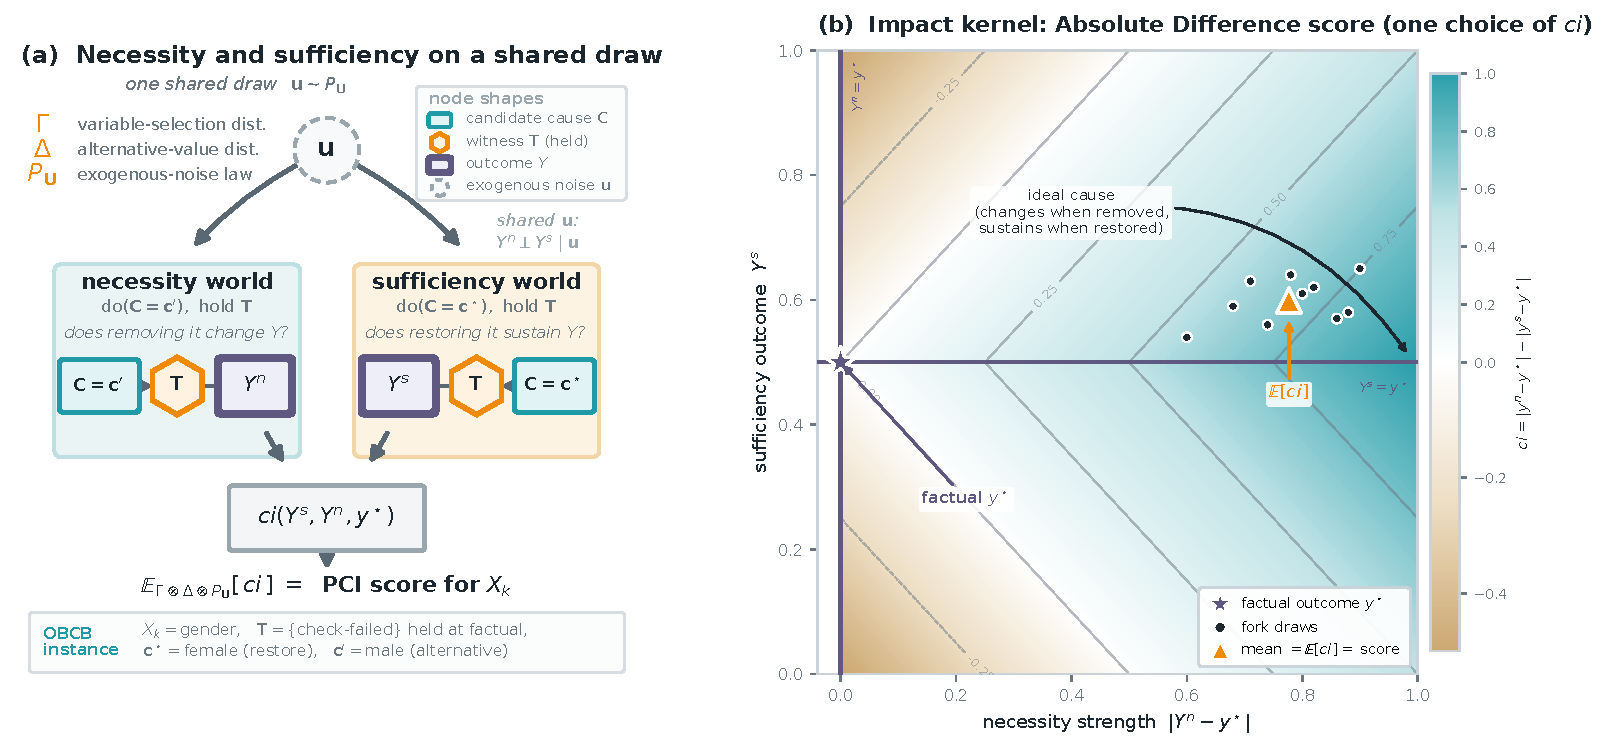
\includegraphics[width=\textwidth]{figures/pci_mechanism.pdf}
\caption{The \ourapproach{} mechanism. \textbf{(a)} For a variable of interest
$X_k$, a single exogenous draw $\mathbf{u}\sim P_{\mathbf{U}}$ together with a
candidate cause set $\mathbf{C}\ni X_k$ and witness set $\mathbf{T}$ from
$\Gamma$ and an alternative value $\mathbf{c}'$ from $\Delta$ defines two
counterfactual worlds on the \emph{same} noise: a \emph{necessity world}
($\mathrm{do}(\mathbf{C}=\mathbf{c}')$, witnesses held) giving $Y^n$, and a
\emph{sufficiency world} ($\mathrm{do}(\mathbf{C}=\mathbf{c}^\star)$, witnesses
held) giving $Y^s$, both drawn against the \emph{same} $(\mathbf{C},\mathbf{T})$
for illustration (the diagonal case of the remark following
Definition~\ref{def:jointnecsuf}). Conditional on $\mathbf{u}$ the two worlds are
independent (the product structure of Definition~\ref{def:jointnecsuf}); the impact
kernel $ci$ scores the pair. \Ourapproach{}'s realised score instead marginalises
$\Gamma$ separately for each world (the independent-product case; see the same
remark) before taking this expectation over $\Delta\otimes P_{\mathbf{U}}$
(Definition~\ref{def:causalimpact}); the two agree here because $ci$ is additively
separable. The strip grounds the schematic in the
OBCB running example. \textbf{(b)} The impact kernel on the \emph{signed} plane
$(Y^n-y^\star,\,Y^s-y^\star)$, shown for the Absolute Difference score
$ci=|y^n-y^\star|-|y^s-y^\star|$, \emph{one} admissible choice of kernel (the
PNS binary score and necessity-only variants are others), before either
deviation is folded by $|\cdot|$. Because $ci$ depends only on the two
absolute deviations, the field is symmetric under an independent sign flip of
either axis: four qualitatively different outcomes, necessity and sufficiency
each landing above or below the factual value, collapse onto the same score
whenever the magnitudes match. The faint cloud is a sample of $(Y^n,Y^s)$
draws (shared with panel~(c)); the four gold points are actual draws, one per
quadrant, with closely matched $|Y^n-y^\star|,|Y^s-y^\star|$, so their nearly
equal $ci$ is a property of the sampled data, not a constructed coincidence.
\textbf{(c)} The same draws' $ci$ values, histogrammed and coloured by sign;
the gold line marks their mean, $\mathbb{E}[ci]$, the \ourapproach{} score for
this variable. This replaces a single scatter-and-mean with the full
distribution the Monte-Carlo estimate is drawn from.}
\label{fig:pci-mechanism}
\end{figure*}

\medskip\noindent Informally, $ci$ is a user-defined scoring rule that translates
the joint sufficiency--necessity measure into a single scalar
(Figure~\ref{fig:pci-mechanism} summarises the whole construction: the two
counterfactual worlds in panel~(a), the kernel that scores them in panel~(b),
and the resulting score as a summary of many such draws in panel~(c)). The
choice is not arbitrary:
the Absolute Difference example below is an instance of L$_1$ distance between outcomes, the
same metric underlying Average Treatment Effect,
 Conditional Average Treatment Effect, and SHAP.
The binary indicator score recovers this as a special
 case when outcomes are binary:
indicators are L$_1$ on $\{0,1\}$. Practitioners
 with reasons to prefer L$_2$ or another
distance measure may substitute it freely; the framework places 
no restriction on $ci$
beyond measurability.

For the OBCB analysis we instantiate $ci$ as the PNS binary score defined in the
following example, with $y^\star = \varname{loan} = 0$. This is the choice that produces
the values in Table~\ref{tab:pci_decomp}.

\begin{example}[PNS for Binary Outcomes]\label{ex:pns_binary}
Assume the outcome $Y$ is binary with $\dom(Y)=\{0,1\}$, and let $y^\star=1$ denote
the factual outcome. Let $Y^s$ and $Y^n$ denote the sufficiency and necessity
outcome variables. Define the causal impact score
\[
ci(y^s,y^n,y^\star)
=
\mathbb{I}\{y^n\neq y^\star\}\,\mathbb{I}\{y^s=y^\star\}.
\]
Then the expected causal impact reduces to
\[
\mathbb{E}\!\left[ci(Y^s,Y^n,1)\right]
=
\mathbb{P}(Y^n=0,\,Y^s=1),
\]
which conceptually coincides with Pearl's probability of necessity and sufficiency (PNS). The alignment is \emph{exact} when $\mathbf{S} = \{X_k\}$, $\mathbf{W}=\emptyset$, and $\dom(X_k)=\{0,1\}$ where, factually, $x_k^\star=1$.
\end{example}

We now illustrate the full computation for Alice's gender attribution using this $ci$.
With $\mathbf{S}=\{\varname{gender},\varname{credit}\}$,
$\mathbf{W}=\{\varname{check\text{-}failed}\}$, $\Gamma_s$ and $\Gamma_w$ uniform,
$\Delta$ a point mass on the alternative binary value, and $y^\star=\varname{loan}=0$,
the exogenous noise $U_\text{check}$ falls into three regions:
\begin{itemize}
\item $u_1$ (prob.\ 0.2): Alice is checked regardless of gender;
  $\varname{check\text{-}failed}=1$ factually.
\item $u_2$ (prob.\ 0.7): Alice is not checked as female but would be as male;
  $\varname{check\text{-}failed}=0$ factually.
\item $u_3$ (prob.\ 0.1): Alice is not checked regardless of gender.
\end{itemize}
In all regions, restoring Alice's factual values always yields a denial, so
$P_k^s(\{0\}\mid\mathbf{u})=\tfrac{2}{3}$ everywhere (four suspect-containing
$(\mathbf{C},\mathbf{T})$ combinations each with $p^\Gamma(\mathbf{C},\mathbf{T})=\tfrac{1}{3}\cdot\tfrac{1}{2}=\tfrac{1}{6}$,
since $\mathbf{S}\cap\mathbf{W}=\emptyset$ here, rejection is vacuous and
$\Gamma$ is just the product of marginals, each contributing probability~1).
The necessity measure varies.

In $u_1$, the witness holds $\varname{check\text{-}failed}=1$.
The four $(\mathbf{C},\mathbf{T})$ contributions, each weighted $\tfrac{1}{6}$, are:
\begin{itemize}
\item[$\circ$] $\mathbf{C}=\{\varname{gender}\}$, $\mathbf{T}=\emptyset$:
  male, $\varname{check\text{-}failed}=1$ propagates structurally
  $\Rightarrow P(\varname{loan}=1)=0.05$.
\item[$\circ$] $\mathbf{C}=\{\varname{gender}\}$,
  $\mathbf{T}=\{\varname{check\text{-}failed}\}$:
  male, witness holds failure
  $\Rightarrow P(\varname{loan}=1)=0.05$.
\item[$\circ$] $\mathbf{C}=\{\varname{gender},\varname{credit}\}$, $\mathbf{T}=\emptyset$:
  male and good credit, check passes
  $\Rightarrow P(\varname{loan}=1)=1.0$.
\item[$\circ$] $\mathbf{C}=\{\varname{gender},\varname{credit}\}$,
  $\mathbf{T}=\{\varname{check\text{-}failed}\}$:
  male and good credit, but witness holds failure
  $\Rightarrow P(\varname{loan}=1)=0.05$.
\end{itemize}
\[ P_k^n(\{1\}\mid u_1)
   = \tfrac{1}{6}(0.05+0.05+1.0+0.05) \approx 0.192. \]

In $u_2$, the witness holds $\varname{check\text{-}failed}=0$.
The four contributions:
\begin{itemize}
\item[$\circ$] $\mathbf{C}=\{\varname{gender}\}$, $\mathbf{T}=\emptyset$:
  male would be checked; $\varname{check\text{-}failed}=1$ propagates structurally
  $\Rightarrow P(\varname{loan}=1)=0.05$.
\item[$\circ$] $\mathbf{C}=\{\varname{gender}\}$,
  $\mathbf{T}=\{\varname{check\text{-}failed}\}$:
  male, witness holds $\varname{check\text{-}failed}=0$, check passes
  $\Rightarrow P(\varname{loan}=1)=1.0$.
\item[$\circ$] $\mathbf{C}=\{\varname{gender},\varname{credit}\}$, $\mathbf{T}=\emptyset$:
  male and good credit, check passes
  $\Rightarrow P(\varname{loan}=1)=1.0$.
\item[$\circ$] $\mathbf{C}=\{\varname{gender},\varname{credit}\}$,
  $\mathbf{T}=\{\varname{check\text{-}failed}\}$:
  male and good credit, witness holds $0$
  $\Rightarrow P(\varname{loan}=1)=1.0$.
\end{itemize}
\[ P_k^n(\{1\}\mid u_2)
   = \tfrac{1}{6}(0.05+1.0+1.0+1.0) \approx 0.508. \]

In $u_3$, male Alice is also not checked ($\varname{check}=0$ regardless of gender),
so all necessity worlds yield denial: $P_k^n(\{1\}\mid u_3)=0$.

Combining, with $ci(y^s,y^n,y^\star)=\mathbb{I}\{y^n\neq y^\star\}\,\mathbb{I}\{y^s=y^\star\}$
and $y^\star=\varname{loan}=0$:
\begin{align*}
\mathrm{PCI}_{\varname{gender}}(\text{Alice})
  &= \mathbb{E}\!\left[ci(Y^s,Y^n,y^\star)\right]
   = \mathbb{P}(Y^n=1,\,Y^s=0) \\
  &= \sum_u p(u)\,P_k^s(\{0\}\mid u)\,P_k^n(\{1\}\mid u) \\
  &= 0.2\times\tfrac{2}{3}\times 0.192
   + 0.7\times\tfrac{2}{3}\times 0.508
   + 0.1\times 0 \\
  &\approx 0.026 + 0.237 = 0.263.
\end{align*}

Table~\ref{tab:pci_decomp} gives the full results for Alice and Bob under these
parameter choices: Pearl's PN/PS/PNS, PCI without witnesses
($\mathbf{W}=\emptyset$), and PCI with the $\varname{check\text{-}failed}$ witness
active, with the latter further decomposed into its necessity and sufficiency
marginals.

\begin{table}[ht]
\centering
\small
\setlength{\tabcolsep}{4pt}
\begin{tabular}{l c c c c c c c}
\toprule
& \multicolumn{3}{c}{Pearl} & PCI & \multicolumn{3}{c}{PCI ($\mathbf{W}=\{\varname{check\text{-}failed}\}$)} \\
\cmidrule(lr){2-4} \cmidrule(lr){6-8}
Person, Variable & PN & PS & PNS & ($\mathbf{W}=\emptyset$) & Necessity & Sufficiency & Total \\
\midrule
Alice (\varname{gender}) & $0.045$ & $1.000$ & $0.045$ & $0.210$
                          & $0.394$ & $0.667$ & $\mathbf{0.263}$ \\
Alice (\varname{credit}) & $0.180$ & $1.000$ & $0.180$ & $0.240$
                          & $0.298$ & $0.667$ & $\mathbf{0.199}$ \\
Bob   (\varname{gender}) & $0.000$ & ---     & $0.000$ & $0.038$
                          & $0.030$ & $0.637$ & $\mathbf{0.019}$ \\
Bob   (\varname{credit}) & $0.900$ & $0.955$ & $0.860$ & $0.228$
                          & $0.188$ & $0.637$ & $\mathbf{0.119}$ \\
\bottomrule
\end{tabular}
\caption{Per-individual responsibility scores for \varname{gender} and \varname{credit}
on $\varname{loan}=0$ in the stochastic OBCB model. Pearl's PN/PS/PNS, PCI without
witnesses ($\mathbf{W}=\emptyset$), and PCI with the \varname{check\text{-}failed}
witness shown side by side; the rightmost three columns decompose PCI($\mathbf{W}=\{\varname{check\text{-}failed}\}$)
into its necessity and sufficiency marginals (their joint expectation is the bold
total). Here the total happens to equal the product of the two marginals because the
sufficiency measure $P_k^s(\cdot\mid\mathbf{u})$ is constant in $\mathbf{u}$ for both
individuals; in general the joint $P_k^{s,n}$ does not factor into the product of its
marginals. Bob's PS for gender is undefined because the conditioning event
$(\text{female}, \text{bad}, \varname{loan}=1)$ has probability zero in the OBCB model;
the PCI marginals are well-defined throughout, since they integrate over $P_{\mathbf{U}}$
rather than conditioning on the factual outcome.}
\label{tab:pci_decomp}
\end{table}

For Alice, PNS and PCI without witnesses both fail \textbf{D-A-rank} (p.~\pageref{desid}):
they rank \varname{credit} above \varname{gender} (0.180 vs.\ 0.045; 0.240 vs.\ 0.210).
PCI with witnesses reverses this (0.263 vs.\ 0.199), satisfying \textbf{D-A-rank} as well
as \textbf{D-A1} and \textbf{D-A2} (both values positive). Holding
\varname{check\text{-}failed} at its factual value blocks the credit-check bottleneck in
noise realizations where Alice was checked, isolating gender's structural role. The
\varname{check\text{-}failed} witness is the decisive ingredient.

For Bob, \textbf{D-B2} and \textbf{D-B-rank} hold under all three methods:
\varname{credit} is ranked above \varname{gender} throughout. \textbf{D-B1} requires
strictly positive attribution for \varname{gender}: PNS returns exactly 0.000 and
therefore fails, because $P(\varname{loan}=1\mid\varname{gender}=\text{female},
\varname{credit}=\text{bad})=0$ makes the counterfactual necessity calculation zero,
missing gender's indirect role in opening the credit evaluation. PCI with witnesses
returns 0.019, correctly capturing this indirect contribution. The cross-individual
desideratum \textbf{D-comp} holds under both PCI (0.263 $>$ 0.019) and PNS
(0.045 $>$ 0.000). A full verification of all seven desiderata is given at the end
of this section.

The PNS and PCI (no witnesses) columns differ even though neither uses witnesses,
because PCI still $\Gamma$-averages over candidate suspect sets.  With
$|\mathbf{S}|=2$ PCI averages over $\{\varname{gender}\}$, $\{\varname{credit}\}$,
and $\{\varname{gender},\varname{credit}\}$ (each weighted $\tfrac{1}{3}$),
whereas PNS evaluates a single counterfactual on one variable at a time.
Property~(i) below establishes that the two agree exactly when $|\mathbf{S}|=1$
(single suspect, no witnesses, binary outcome), whereas the OBCB setup uses
$|\mathbf{S}|=2$ deliberately, to demonstrate joint-subset attribution.

% \begin{definition}[Causal impact and its push-forward]
% Let $y^s$ denote the outcome in the \emph{sufficiency world}, $y^n$ denote the outcome in the \emph{necessity world}, and $y^\star$ the outcome in the factual world. By construction, these are independent conditional on $\mathbf{u}$, and so we get the joint:
% \begin{align}
%  p(\langle y^s, y^n \rangle \mid \mathbf{u})  & = p^s_k(y^s \mid \mathbf{u}) \; {p}^n_k(y^n \mid \mathbf{u}).
% \end{align}

% \noindent which also generates a push-forward on any causal impact scoring function $ci(y^s, y^n, y^\star)$, whose expectation is a summary of causal impact.
% \begin{align}\label{eq:score}
% \mathbb{E}_{\mathbf{u}}\Big[\, \mathbb{E}_{y^s, y^n \mid \mathbf{u}} \big[ ci(y^s, y^n, y^\star) \big] \,\Big]
% =\\ \iiint  ci(y^s, y^n, y^\star) \; p^s_k(y^s \mid \mathbf{u}) \; p^n_k(y^n \mid \mathbf{u}) p(\mathbf{u}) 
%    \, dy^s \, dy^n \, d\mathbf{u}. \nonumber
% \end{align}
% \end{definition}

% With this in place, we can characterize a number of causal impact measures by first defining a \emph{causal impact function} as the expectation of a causal impact function taken with respect to the joint measure on factual and counterfactual outcomes.

\subsection{Continuous Outcomes and the General Causal Impact Function}
\label{sub:continuous_ci}

\noindent The causal impact function $ci$ is a user-defined component of \ourapproach, and different choices encode different causal questions. In the benchmarking experiments of \cref{sec:ac_benchmark}, we instantiate $ci$ using only the necessity component, since Halpern’s actual causality has no sufficiency counterpart: necessity-only attribution allows a direct parallel comparison. The full framework incorporating both $Y^s$ and $Y^n$ is instantiated in the PNS binary
example above and in the Absolute Difference example below; the OBCB analysis of this
section (Tables~\ref{tab:pci_decomp}--\ref{tab:desiderata}) provides a concrete
validation, since the PNS binary $ci$ jointly conditions on $Y^s=y^\star$ and
$Y^n\neq y^\star$ and it is precisely this combination that produces the correct
\textbf{D-A-rank} ordering. Further experiments using the full $ci$ on continuous outcomes are presented in
the signal-with-mediation example (Section~\ref{sec:signal}), the synthetic
evaluation (\cref{sub:synthetic}), and the SIR benchmark
(\cref{sec:sir_benchmark}).

When the outcome variable $Y$ is continuous rather than binary, indicators are replaced by a distance-based score that measures how far the necessity and sufficiency worlds land from the factual value $y^\star$.
The natural choice, paralleling L$_1$-based scores such as ATE and SHAP, is the absolute difference.

\begin{example}[Absolute Difference Impact Score] \label{ex:absolute_score}
We can develop an analogous measure for continuous outcomes where we increase attribution with distance from the factual value $y^\star$ in the necessity world and decrease impact with distance to the factual value in the sufficiency world.
\begin{align*}
ci(y^s, y^n, y^\star) & = \vert y^n - y^\star \vert   - \vert y^s - y^\star \vert.
\end{align*}
\end{example}

\noindent Two one-sided instances of this score recur in the experiments: a
necessity-only $ci_N$ and a sufficiency-only $ci_S$ (\cref{sub:synthetic}), whose sum
returns the absolute-difference $ci$ above. Each is a choice of $ci$ in the sense of
Definition~\ref{def:causalimpact}.

With the full machinery in place (structural model, variable selection, alternative
value distribution, joint necessity-sufficiency measure, and causal impact function),
\ourapproach delivers the following properties.
\begin{enumerate}[label=(\roman*)]
\item \textbf{Generalisation of PN/PS/PNS.} When $\mathbf{S}=\{X_k\}$,
  $\mathbf{W}=\emptyset$, and $\dom(X_k)=\{0,1\}$, the PNS binary $ci$ recovers Pearl's
  probability of necessity and sufficiency exactly; PN and PS are recovered by the
  corresponding one-sided $ci$ choices.
\item \textbf{Connection to actual causality.} For suitable $\Gamma$
  and $\Delta$, \ourapproach recovers Halpern's actual causality judgements
  (Section~\ref{sec:relation_with_ac}).
\item \textbf{Necessity--sufficiency decomposition.} $P_k^s$ and $P_k^n$ are defined and
  interpretable independently; practitioners may choose a $ci$ that uses either alone
  or both, depending on whether the causal question concerns necessity, sufficiency,
  or both.
\item \textbf{Witness-mediated symmetry breaking.} Holding intermediate variables fixed
  via $\mathbf{W}$ disambiguates overdetermination and undercutting scenarios where
  necessity-only methods assign equal or zero attribution, as demonstrated above for
  Alice and Bob, and further developed in Section~\ref{sec:shap_examples} (SHAP and
  Causal SHAP comparison), \cref{sub:synthetic} (synthetic overdetermination
  and undercutting archetypes), and \cref{sec:ac_benchmark} (witness ablation
  on the scaled throwing problem).
\item \textbf{Composability.} $\Gamma$, $\Delta$, and $ci$ are probability distributions
  and a measurable function respectively; they slot naturally into Bayesian pipelines,
  accept posteriors as inputs, and admit Monte Carlo estimation without modification to
  the core formalism.
\end{enumerate}

\subsection{Back to the Running Example: Verifying the Desiderata}
\label{sub:verify_desiderata}

Table~\ref{tab:desiderata} verifies the seven desiderata introduced at the start of this
section (p.~\pageref{desid}) against the values in Table~\ref{tab:pci_decomp}.
PCI with witnesses satisfies all seven; PCI without witnesses fails \textbf{D-A-rank};
PNS fails \textbf{D-A-rank} and \textbf{D-B1}.
(The table uses the shorthand $|R(V\mid\text{person})|$ for
$|R(V\rightsquigarrow\varname{loan}\mid\text{person})|$.)

\begin{table}[ht]
\centering
\resizebox{\linewidth}{!}{%
\begin{tabular}{lccc}
\toprule
Desideratum & PNS & PCI (no wit.) & PCI (with wit.) \\
\midrule
\textbf{D-A1}: $|R(\varname{gender}\mid\text{Alice})| > 0$
  & $\checkmark$\ 0.045 & $\checkmark$\ 0.210 & $\checkmark$\ 0.263 \\
\textbf{D-A2}: $|R(\varname{credit}\mid\text{Alice})| > 0$
  & $\checkmark$\ 0.180 & $\checkmark$\ 0.240 & $\checkmark$\ 0.199 \\
\textbf{D-A-rank}: $|R(\varname{gender}\mid\text{Alice})| > |R(\varname{credit}\mid\text{Alice})|$
  & $\times$\ $0.045 {<} 0.180$
  & $\times$\ $0.210 {<} 0.240$
  & $\checkmark$\ $0.263 {>} 0.199$ \\
\textbf{D-B1}: $|R(\varname{gender}\mid\text{Bob})| > 0$
  & $\times$\ 0.000 & $\checkmark$\ 0.038 & $\checkmark$\ 0.019 \\
\textbf{D-B2}: $|R(\varname{credit}\mid\text{Bob})| > 0$
  & $\checkmark$\ 0.860 & $\checkmark$\ 0.228 & $\checkmark$\ 0.119 \\
\textbf{D-B-rank}: $|R(\varname{credit}\mid\text{Bob})| > |R(\varname{gender}\mid\text{Bob})|$
  & $\checkmark$\ $0.860 {>} 0.000$
  & $\checkmark$\ $0.228 {>} 0.038$
  & $\checkmark$\ $0.119 {>} 0.019$ \\
\textbf{D-comp}: $|R(\varname{gender}\mid\text{Alice})| > |R(\varname{gender}\mid\text{Bob})|$
  & $\checkmark$\ $0.045 {>} 0.000$
  & $\checkmark$\ $0.210 {>} 0.038$
  & $\checkmark$\ $0.263 {>} 0.019$ \\
\bottomrule
\end{tabular}}
\caption{Verification of the seven desiderata (p.~\pageref{desid}) against the values in
Table~\ref{tab:pci_decomp}. PCI with witnesses satisfies all seven; PCI without witnesses
fails \textbf{D-A-rank}; PNS fails \textbf{D-A-rank} and \textbf{D-B1}.}
\label{tab:desiderata}
\end{table}

\medskip\noindent\textit{PNS fails \textbf{D-A-rank} and \textbf{D-B1}. The D-A-rank
failure reflects that without a \varname{check\text{-}failed} witness,
necessity-based attribution cannot distinguish Alice's gender (which blocked the
evaluation entirely) from her credit (which would only have mattered had she been
evaluated). The D-B1 failure reflects that PNS assigns Bob's gender exactly zero:
because $P(\varname{loan}=1\mid\text{female},\text{bad})=0$,
the counterfactual necessity calculation returns zero, missing gender's indirect role in
opening the credit evaluation. The \varname{check\text{-}failed} witness resolves both.}

To close this section, it is worth comparing PCI's decomposition with the one already
present in Pearl's framework. Pearl's framework defines three related but distinct
binary scores: the probability of necessity
$\mathrm{PN} = P(Y_{x'} = y' \mid X = x^\star, Y = y^\star)$, the probability of sufficiency
$\mathrm{PS} = P(Y_{x^\star} = y^\star \mid X = x', Y = y')$, and their joint
$\mathrm{PNS} = P(Y_{x^\star} = y^\star, Y_{x'} = y')$. The first two are conditional
probabilities; $\mathrm{PNS}$ is unconditional, and the three satisfy
$\mathrm{PNS} = \mathrm{PN}\cdot P(Y_{x^\star}=y^\star) = \mathrm{PS}\cdot P(Y_{x'}=y')$ rather
than $\mathrm{PNS} = \mathrm{PN}\cdot\mathrm{PS}$ (which would require
$Y_{x^\star}\perp Y_{x'}$, an assumption typically violated since the two potential
outcomes share exogenous noise). PCI admits a related split: with
$ci = \mathbb{I}\{y^n \neq y^\star\}\,\mathbb{I}\{y^s = y^\star\}$,
\[
\mathbb{E}[ci(Y^s, Y^n, y^\star)]
= \int P^s_k(\{y^\star\}\mid\mathbf{u})\,P^n_k(\{1{-}y^\star\}\mid\mathbf{u})\,dP_{\mathbf{U}},
\]
giving a \emph{sufficiency marginal} and a \emph{necessity marginal} that record how
often, on average, restoring the factual values of a suspect set containing $X_k$
reproduces the factual outcome, and how often substituting alternatives overturns it.
The two marginals are independent given $\mathbf{u}$.

The components are not identical to Pearl's: $\mathrm{PN}$ and $\mathrm{PS}$ condition
on the factual outcome and consider a single counterfactual flip; PCI's marginals
integrate over $P_{\mathbf{U}}$, average over suspect sets weighted by $\Gamma$, and
hold the witness configurations fixed when active. Table~\ref{tab:pci_decomp} (presented
earlier) places both decompositions side by side for \varname{gender} and
\varname{credit}.


For Alice's gender, $\mathrm{PN} = 0.045$ is the bare probability that a male with bad
credit would have been approved; PCI's necessity marginal is $0.394$, nearly an order of
magnitude higher, because the \varname{check\text{-}failed} witness keeps the
credit-check bottleneck active when the male counterfactual would otherwise have been
checked and might still have failed, structural information that the unconditional
$\mathrm{PN}$ cannot register. For Bob's gender, $\mathrm{PN}$ is exactly $0$ (a female
with bad credit cannot be approved in this model) and $\mathrm{PS}$ is undefined; PCI's
marginals remain well-defined at $0.030$ and $0.637$, recovering the indirect role of
gender in opening the evaluation.

The next section turns from comparing PCI with Pearl's family of counterfactual scores
to comparing it with the SHAP family, methods grounded in cooperative game theory
rather than in structural counterfactual reasoning.
Section~\ref{sec:shap_examples} re-runs the OBCB analysis under plain and Causal
SHAP, then introduces a continuous mediation example where the two SHAP variants
diverge from each other and from PCI, with explicit desiderata recorded throughout.


\section{Examples and comparison to SHAP and Causal SHAP}\label{sec:shap_examples}

\paragraph{Where we are.} Section~\ref{sec:causal_impact} defined \ourapproach
and verified, on Alice and Bob, that the resulting attribution satisfies all seven
desiderata of that section, where PN/PS/PNS fail at least two. The natural next
question is how \ourapproach compares to the dominant practical alternative for
feature attribution in the ML literature --- SHAP and Causal SHAP --- since these
are the tools practitioners typically reach for. This section runs that comparison
on two examples, recording where each method passes or fails an explicit
desideratum. We first define SHAP and Causal SHAP formally
(Section~\ref{sec:shap_defs}), then re-run OBCB
(Section~\ref{sec:obcb_shap}) --- where the two SHAP variants coincide because the
feature set is exogenous, so the divergence between PCI and SHAP is the only
contrast to draw. We then introduce a continuous mediation example
(Section~\ref{sec:signal}) where plain and Causal SHAP do diverge --- one
desideratum (D-YX) is fixed by the interventional correction, others (D-YM,
D-MX, D-MXY) are not --- and tabulate the desiderata in
Section~\ref{sec:shap_signal}. Section~\ref{sec:shap_summary} traces every
failure to one of three structural gaps in the SHAP framework that PCI's witness
mechanism, suspect-set distribution $\Gamma_s$, and realised-outcome reference
jointly close.

Shapley values have become one of the most widely used tools for explaining the
predictions of complex machine learning models. Grounded in cooperative game theory,
they provide a principled decomposition of a model's prediction into additive
contributions from individual features.
\citet{janzing2020feature} argued that the conditional expectation in plain SHAP is the
conceptually wrong way to model feature removal --- a dropped feature should be
marginalised under a $do$-intervention, not under conditioning.
\citet{heskes2020causal} propose Causal SHAP, which implements this prescription by
replacing the observational marginal used for features outside the active coalition
with an interventional distribution: when a dropped feature is causally downstream of
a coalition member, its distribution under the intervention differs from its marginal,
and Causal SHAP corrects for this using Pearl's do-calculus.\footnote{%
A different counterfactual line is taken by \citet{sharma2022cfshapley}, whose
CF-Shapley values use a structural causal model to attribute the change in a metric
from a single fixed reference $x^{\text{ref}}$ to the observed $x$:
$\phi_j \propto \sum_{\mathcal{S}\subseteq N\setminus\{j\}}
[f(x_\mathcal{S}, x_j^{\text{ref}}) - f(x_\mathcal{S}, x_j)]$.
This is the closest neighbour to \ourapproach{} in spirit --- single contrastive
scenario, $do$-style intervention --- and differs in three ways.
\emph{(i)} CF-Shapley commits to one reference $x^{\text{ref}}$, while \ourapproach{}
integrates over an alternative-value distribution $\Delta(\mathbf{x})$ and need not pick
a single contrast.
\emph{(ii)} CF-Shapley returns a one-axis contrast
$f(\cdot, x_j^{\text{ref}}) - f(\cdot, x_j)$, while \ourapproach{} reports a joint
$(Y^s, Y^n)$ measure and applies a user-chosen $ci$, decomposing necessity and
sufficiency separately.
\emph{(iii)} CF-Shapley has no witness mechanism, so it cannot break the
overdetermination and undercutting symmetries that \ourapproach{}'s witness set
$\mathbf{W}$ resolves on the OBCB and signal walkthroughs of this section.}
Formal definitions of both are given in Section~\ref{sec:shap_defs}.

Despite this repair, both methods share deeper limitations. First, both plain and
Causal SHAP can assign non-zero responsibility to variables that play no causal role
with respect to the target --- attribution can run against the direction of the causal
graph, a failure the interventional correction does not address. Second, both methods
explain a model's predicted output averaged over the population, not the individual
factual outcome of a specific person: when the goal is \emph{causal responsibility
attribution}, this produces further failures that are not always made explicit in the
literature. The first limitation will surface in our signal example as violations of
D-YX, D-YM, and D-MX; the second will surface in OBCB as the D-A-rank overdetermination
effect, and in the signal example as Instance~2's budget collapse when the prediction
equals its baseline.

We trace these failures through two examples, comparing plain SHAP, Causal SHAP, and
PCI against the desiderata of Section~\ref{sec:motivations} and some further desiderata related to the example we 
will employ. We first return to the
OBCB model: it permits exact analytic computation and the desiderata are already
known. In OBCB the feature set contains only exogenous roots, so plain and Causal
SHAP coincide --- the comparison is short. We then turn to a continuous mediation
example where downstream variables are observable model inputs; there the two methods
diverge, and we examine what Causal SHAP fixes and what it does not.

\subsection{SHAP and Causal SHAP}\label{sec:shap_defs}

In this section $\mathcal{S} \subseteq N$ denotes a SHAP coalition (a subset of features held
to their factual values during evaluation), playing the same role here that
$\mathbf{C} \subseteq \mathbf{S}$ played in Section~\ref{sec:causal_impact}. We use the
calligraphic $\mathcal{S}$ to keep the SHAP coalition typographically distinct from PCI's
suspect set $\mathbf{S}$ on the printed page; the SHAP literature's plain $S$ is the same
object.

\begin{definition}[SHAP]
A cooperative game is a pair $(N, v)$,
where $N = \{1, \ldots, n\}$ is the set of players and $v: 2^N \to \mathbb{R}$
is the \emph{characteristic function} mapping each subset
(coalition) $\mathcal{S} \subseteq N$ to the value that coalition can produce. The Shapley value
\citep{shapley1953} is the unique attribution satisfying four axioms:
\begin{enumerate}
\item \textbf{Efficiency}: $\sum_i \phi_i = v(N) - v(\emptyset)$
\item \textbf{Symmetry}: If $v(\mathcal{S} \cup \{i\}) = v(\mathcal{S} \cup \{j\})$ for all $\mathcal{S}$, then
      $\phi_i = \phi_j$
\item \textbf{Dummy}: If $v(\mathcal{S} \cup \{i\}) = v(\mathcal{S})$ for all $\mathcal{S}$, then $\phi_i = 0$
\item \textbf{Linearity}: For two games $v_1, v_2$: $\phi_i(\alpha_1 v_1 + \alpha_2 v_2)
      = \alpha_1 \phi_i(v_1) + \alpha_2 \phi_i(v_2)$
\end{enumerate}
The unique solution is:
\begin{equation}
\phi_i = \sum_{\mathcal{S} \subseteq N \setminus \{i\}}
\frac{|\mathcal{S}|!\,(|N|-|\mathcal{S}|-1)!}{|N|!}
\bigl[v(\mathcal{S} \cup \{i\}) - v(\mathcal{S})\bigr]
\label{eq:shapley}
\end{equation}
The weight $\frac{|\mathcal{S}|!(|N|-|\mathcal{S}|-1)!}{|N|!}$ equals the probability that, in a uniformly
random ordering of all players, exactly the members of $\mathcal{S}$ precede $i$. Equivalently,
$\phi_i$ is the average marginal contribution of $i$ across all orderings.
\citet{lundberg2017unified} apply Shapley values to explain model predictions by taking
players to be input features, and the characteristic function to be the expected model
output given a subset of features:
\begin{equation}
v(\mathcal{S}) = \mathbb{E}_{X_{\bar{\mathcal{S}}}}\bigl[f(X_{\mathcal{S}} = x_{\mathcal{S}},\, X_{\bar{\mathcal{S}}})\bigr]
\end{equation}
\noindent where $\bar{\mathcal{S}} = N \setminus \mathcal{S}$ and missing features are marginalized over
their marginal distribution.
\end{definition}

\medskip\noindent Causal SHAP replaces the characteristic function with an
interventional expectation \citep{heskes2020causal}:

\begin{definition}[Causal SHAP]\label{def:causalshap}
\begin{equation}
v_{\text{causal}}(\mathcal{S}) = \mathbb{E}\bigl[f(X) \mid do(X_{\mathcal{S}} = x_{\mathcal{S}})\bigr]
= \int P(X_{\bar{\mathcal{S}}} \mid do(X_{\mathcal{S}} = x_{\mathcal{S}}))\, f(X_{\bar{\mathcal{S}}}, x_{\mathcal{S}})\, dX_{\bar{\mathcal{S}}}
\label{eq:causal_v}
\end{equation}
By the rules of do-calculus, intervening on $X_{\mathcal{S}}$ only affects the distribution of
descendants of $X_{\mathcal{S}}$. For non-descendants, $P(X_j \mid do(X_{\mathcal{S}} = x_{\mathcal{S}})) = P(X_j)$.
Writing $X_{\bar{\mathcal{S}},\,\mathrm{nd}}$ for the features in $\bar{\mathcal{S}}$ that are not
descendants of any member of $\mathcal{S}$, and $X_{\bar{\mathcal{S}},\,\mathrm{d}}$ for those that are,
equation~\eqref{eq:causal_v} is equivalent to:
\begin{equation}
v_{\text{causal}}(\mathcal{S}) = \mathbb{E}_{X_{\bar{\mathcal{S}},\,\mathrm{nd}} \sim P(\cdot),\;
X_{\bar{\mathcal{S}},\,\mathrm{d}} \sim P(\cdot \mid do(X_{\mathcal{S}}=x_{\mathcal{S}}))}\bigl[f(X_{\bar{\mathcal{S}}}, x_{\mathcal{S}})\bigr]
\end{equation}
The Shapley formula~\eqref{eq:shapley} is otherwise unchanged. The method retains all
four Shapley axioms.
\end{definition}

\medskip\noindent
At the level of subset weighting alone, \ourapproach{} (with $J=1$, $K=|\mathbf{S}|$) and
SHAP are not distinguishable: $\Gamma$'s subset weights match the Shapley kernel. The
distinction lies in the integrand. SHAP averages marginal contributions using the
observational conditional
$\mathbb{E}[f(\mathbf{X}_{\mathcal{S}} = \mathbf{x}_{\mathcal{S}}, \mathbf{X}_{\bar{\mathcal{S}}})]$, marginalising over the
empirical distribution of non-coalition features; a feature merely correlated with a true
cause can therefore receive positive attribution. \ourapproach{} evaluates counterfactual
outcomes
$P(Y \in A \mid \mathbf{u},\, \mathrm{do}(\mathbf{C}=\mathbf{c}',\,\mathbf{T}=\mathbf{t}^\star))$
computed via the structural model, so attribution flows only along genuine causal paths.
The witness mechanism adds a further distinction: by holding intermediate variables fixed,
\ourapproach{} can resolve overdetermination and undercutting scenarios where SHAP assigns
equal or incorrect attribution. The remainder of this section makes both points concrete on
two examples.

\subsection{OBCB: SHAP and Causal SHAP}\label{sec:obcb_shap}

To apply the SHAP and Causal SHAP definitions of Section~\ref{sec:shap_defs}
to OBCB we must specify both a feature set $N$ and a function $f$ on the joint
feature space; the value functions and Shapley sums are derived from these.
The natural choice for $f$ is the conditional expectation of the outcome,
$f(x_N)=\mathbb{E}[\varname{loan}\mid X_N=x_N]$. But the OBCB PSCM has five
variables --- $\varname{gender}$, $\varname{credit}$, $\varname{check}$,
$\varname{check\text{-}failed}$, $\varname{loan\_if\_checked}$ --- so the
choice of $N$ is non-trivial. Two options are natural:
\begin{itemize}
\item \textbf{Option A: two upstream roots.}
$N=\{\varname{gender},\varname{credit}\}$. Both features are exogenous; the
three internal variables ($\varname{check}$, $\varname{check\text{-}failed}$,
$\varname{loan\_if\_checked}$) are integrated out inside $f$. This is the
smallest sufficient feature set and matches the way the model is normally
described: predict approval from gender and credit.
\item \textbf{Option B: two roots plus the mediator.}
$N'=\{\varname{gender},\varname{credit},\varname{check\text{-}failed}\}$.
The mediator becomes an observable model input, the same status it has in the
signal-with-mediation example (\S\ref{sec:signal}). This is the comparison
PCI's witness mechanism naturally invites: PCI accesses
$\varname{check\text{-}failed}$ as a witness, so allowing SHAP to access it as
a feature is the fair foil.
\end{itemize}
We work through both. Option~A is simpler and exposes the qualitative failures
of plain SHAP. Option~B then asks whether admitting the mediator rescues Causal
SHAP.

\medskip\noindent\textbf{Option~A: two upstream roots.}
Here $f(g,c)=P(\varname{loan}=1\mid g,c)$ takes values
$f(\text{F},\text{bad})=0.000$, $f(\text{F},\text{good})=0.180$,
$f(\text{M},\text{bad})=0.045$, $f(\text{M},\text{good})=0.900$, with the three
internal variables integrated out. We apply SHAP to the rejection probability
$g(x)=1-f(x)$ for Alice and Bob from Example~\ref{ex:obcb_stochastic},
attributing responsibility for the denial outcome.\footnote{Because $g=1-f$,
the characteristic functions satisfy $v_g(\mathcal{S})=1-v_f(\mathcal{S})$ and
$\phi^g_i=-\phi^f_i$; we compute $\phi^f$ and flip signs. With $|N|=2$ and
uniform marginals $P(\varname{gender})=P(\varname{credit})=\tfrac{1}{2}$,
equation~\eqref{eq:shapley} reduces to
$\phi_i = \tfrac{1}{2}[v(\{i\})-v(\emptyset)] + \tfrac{1}{2}[v(N)-v(N\!\setminus\!\{i\})]$.}
By the SHAP definition (and equivalently by Definition~\ref{def:causalshap}
once we note that no dropped feature is a descendant of any coalition member),
the value function on the 2-feature game is
\[
v(\mathcal{S}) \;=\; \mathbb{E}\!\left[f(X)\,\big|\,X_{\mathcal{S}} = x_{\mathcal{S}}^\star\right]
\;=\; \sum_{x_{N\setminus S}\in\{0,1\}^{|N\setminus S|}} P(X_{N\setminus S}=x_{N\setminus S})\,f(x_{\mathcal{S}}^\star,\,x_{N\setminus S}).
\]
Under independent uniform marginals
$P(\varname{gender})=P(\varname{credit})=\tfrac{1}{2}$ this specialises to
\begin{align*}
v(\emptyset)                              &= \tfrac{1}{4}\sum_{g,c\in\{0,1\}} f(g,c),
&&[\text{both dropped: weight } \tfrac{1}{2}\cdot\tfrac{1}{2}] \\
v(\{\varname{gender}\})                   &= \tfrac{1}{2}\!\left[f(g^\star,0)+f(g^\star,1)\right],
&&[\text{only credit dropped: weight } P(c) = \tfrac{1}{2}] \\
v(\{\varname{credit}\})                   &= \tfrac{1}{2}\!\left[f(0,c^\star)+f(1,c^\star)\right],
&&[\text{only gender dropped: weight } P(g) = \tfrac{1}{2}] \\
v(\{\varname{gender},\varname{credit}\})  &= f(g^\star,c^\star).
&&[\text{nothing dropped: no average}]
\end{align*}
Plugging in the four values of $f$ listed at the start of Option~A yields
Table~\ref{tab:vS_optionA}; pushing those through the closed-form Shapley above
gives the magnitudes in Table~\ref{tab:shap_obcb}, which compares against PNS
and PCI.

\begin{table}[h]
\centering
\begin{tabular}{lcc}
\toprule
$\mathcal{S}$ & $v(\mathcal{S})$ for Alice & $v(\mathcal{S})$ for Bob \\
\midrule
$\emptyset$                              & $0.281$ & $0.281$ \\
$\{\varname{gender}\}$                   & $0.090$ & $0.473$ \\
$\{\varname{credit}\}$                   & $0.023$ & $0.023$ \\
$\{\varname{gender},\varname{credit}\}$  & $0.000$ & $0.045$ \\
\bottomrule
\end{tabular}
\caption{Coalition values $v(\mathcal{S})=\mathbb{E}[f(X)\mid X_{\mathcal{S}}=x_{\mathcal{S}}^\star]$ for the
2-feature game ($N=\{\varname{gender},\varname{credit}\}$).
$v(\emptyset)=\mathbb{E}[f(X)]=0.281$ is the population baseline; $v(N)$ is
the factual prediction $f(x^\star)$. Plain SHAP and Causal SHAP coincide on
this game (neither feature is downstream of the other), so a single column
suffices per individual.}
\label{tab:vS_optionA}
\end{table}

\begin{table}[h]
\centering
\begin{tabular}{llcccc}
\toprule
Person & Feature & PNS & SHAP & PCI (no witnesses) & PCI (with witnesses) \\
\midrule
Alice & \varname{gender} & 0.045 & \phantom{$-$}0.107 & 0.210 & \textbf{0.263} \\
Alice & \varname{credit} & 0.180 & \phantom{$-$}0.174 & 0.240 & \textbf{0.199} \\
Bob   & \varname{gender} & 0.000 & $-$0.107           & 0.038 & \textbf{0.019} \\
Bob   & \varname{credit} & 0.860 & \phantom{$-$}0.343 & 0.228 & \textbf{0.119} \\
\bottomrule
\end{tabular}
\caption{Responsibility attributions for Alice and Bob. SHAP values are signed
($\phi^g_i$ for $P(\varname{loan}=0\mid x)$); desiderata compare magnitudes
$|\cdot|$. PNS and PCI values from Table~\ref{tab:pci_decomp}.}
\label{tab:shap_obcb}
\end{table}

SHAP fails two desiderata. The primary failure is \textbf{D-A-rank}: Alice's 
credit outranks her gender ($0.174 > 0.107$). This is an overdetermination
effect: \varname{credit}=bad correlates with the \varname{check\text{-}failed}
mechanism that blocked Alice's credit evaluation, so SHAP's observational
marginalization inflates credit attribution above gender's. PCI includes the factual
\varname{check\text{-}failed} value directly, isolating gender's upstream causal
role and recovering the correct ranking. PNS fails \textbf{D-A-rank} for the same reason;
it also fails \textbf{D-B1} by returning exactly zero for Bob's gender (see
Table~\ref{tab:desiderata}).

The second SHAP failure is \textbf{D-comp}: $|\phi^g_{\varname{gender}}|=0.107$
for both Alice and Bob. But gender played a strictly larger causal role in Alice's
rejection than in Bob's. For Alice, \varname{gender}=female was sufficient on its
own to produce rejection --- it blocked the credit evaluation entirely, so her
credit was never a factor. For Bob, \varname{gender}=male was a facilitating
condition: it triggered the credit check, but \varname{credit}=bad was the actual
driver of the denial. SHAP cannot distinguish these because it measures how far
each feature value deviates from the population prediction mean --- female and
male are equidistant deviations in opposite directions, so they receive equal
magnitude regardless of their individual causal weight. This is an instance of a
deeper limitation: SHAP explains predicted outputs, not individual factual
outcomes, which we examine further in Section~\ref{sec:signal}.

Causal SHAP coincides exactly with plain SHAP under Option~A: both features
are exogenous roots, so
$P(\varname{credit}\mid do(\varname{gender}=g))=P(\varname{credit})$ and vice
versa, no dropped feature is a descendant of any coalition member, and
$v_{\mathrm{causal}}(\mathcal{S})=v_{\mathrm{plain}}(\mathcal{S})$ for every coalition. Option~A
therefore reduces to a single SHAP analysis, and the failures
above belong to both methods.

\medskip\noindent\textbf{Option~B: two roots plus the mediator.}
Throughout this subsection we abbreviate $\varname{gender}$, $\varname{credit}$, and
$\varname{check\text{-}failed}$ as $g$, $c$, and $cf$ in mathematical expressions and table
cells; running prose retains the full names.
Now we admit \varname{check\text{-}failed} as a third model input and apply
both methods to the 3-feature game $N'=\{\varname{gender},\varname{credit},\varname{check\text{-}failed}\}$.
This requires defining $f$ on $\{0,1\}^3$ rather than on $\{0,1\}^2$. The
natural observational extension is again the conditional expectation
$\tilde f(g,c,cf)=\mathbb{E}[\varname{loan}\mid \varname{gender}=g,\,\varname{credit}=c,\,\varname{check\text{-}failed}=cf]$.
This is well defined for three of the four $(c,cf)$ combinations, but not the
fourth: a failed check requires that a check happened \emph{and} the credit
was bad, so $\varname{check\text{-}failed}=1$ together with
$\varname{credit}=\text{good}$ is impossible under the PSCM and has no
observational data to condition on. We leave $\tilde f$ undefined on this cell.

Both methods need a value function $v(\mathcal{S})$: the expected value of $\tilde f$
when the features in $\mathcal{S}$ are held at their factual values $x_{\mathcal{S}}^\star$ and the
remaining features are averaged out. The methods differ in how that average
is taken. Plain SHAP averages over each dropped feature using its own
observational marginal $P(X_i)$, with the dropped features treated as
independent of one another. Causal SHAP averages over the joint distribution
the PSCM produces under the intervention $do(X_{\mathcal{S}} = x_{\mathcal{S}}^\star)$, so the dropped
features keep whatever joint dependencies the PSCM imposes on them. Whether
either average ever lands on the impossible cell $(c{=}1, cf{=}1)$ --- and so
whether $v(\mathcal{S})$ is finite --- depends on both the method and on which features
are held fixed at which factual values. Table~\ref{tab:vS_optionB} works out
all eight coalition values for both individuals.

\begin{table}[h]
\centering
\small
\begin{tabular}{l cc cc}
\toprule
& \multicolumn{2}{c}{Alice $(g,c,cf){=}(0,0,0)$} & \multicolumn{2}{c}{Bob $(g,c,cf){=}(1,0,1)$} \\
\cmidrule(lr){2-3} \cmidrule(lr){4-5}
$\mathcal{S}$ & $v_{\mathrm{plain}}$ & $v_{\mathrm{causal}}$ & $v_{\mathrm{plain}}$ & $v_{\mathrm{causal}}$ \\
\midrule
$\emptyset$    & \textbf{NaN} & $0.281$ & \textbf{NaN} & $0.281$ \\
$\{g\}$        & \textbf{NaN} & $0.090$ & \textbf{NaN} & $0.473$ \\
$\{c\}$        & $0.007$      & $0.023$ & $0.007$      & $0.023$ \\
$\{cf\}$       & $0.270$      & $0.270$ & \textbf{NaN} & \textbf{NaN} \\
$\{g,c\}$      & $0.000$      & $0.000$ & $0.014$      & $0.045$ \\
$\{g,cf\}$     & $0.090$      & $0.090$ & \textbf{NaN} & \textbf{NaN} \\
$\{c,cf\}$     & $0.000$      & $0.000$ & $0.025$      & $0.025$ \\
$N'$           & $0.000$      & $0.000$ & $0.050$      & $0.050$ \\
\bottomrule
\end{tabular}
\caption{Coalition values for the 3-feature game
$N' = \{\varname{gender},\varname{credit},\varname{check\text{-}failed}\}$.
Bold \textbf{NaN} entries flag coalitions whose value function evaluates
$\tilde f$ at the impossible cell $(c{=}1,cf{=}1)$ with positive weight.
Plain SHAP and Causal SHAP coincide whenever neither $\varname{credit}$ nor
$\varname{check\text{-}failed}$ is dropped, since the only structural coupling
in the model is between these two; they diverge whenever one is in $\mathcal{S}$ and the
other is not.}
\label{tab:vS_optionB}
\end{table}

\textbf{Plain SHAP.}
Plain SHAP treats $\varname{credit}$ and $\varname{check\text{-}failed}$ as
independent, so whenever both are dropped from the coalition the average runs
over all four $(c, cf)$ combinations, with the impossible $(c{=}1, cf{=}1)$
combination receiving weight
$P(c{=}1)\cdot P(cf{=}1) = 0.5\cdot 0.275 \approx 0.140$ ---
the same nonzero weight as any other corner. For Alice, both $\varname{credit}$ and
$\varname{check\text{-}failed}$ are dropped at $\mathcal{S}\in\{\emptyset,\{\varname{gender}\}\}$,
the first two NaN
entries in Table~\ref{tab:vS_optionB}. For Bob the same two coalitions fail,
and two more break for an additional reason: at
$\mathcal{S}=\{\varname{check\text{-}failed}\}$ and
$\mathcal{S}=\{\varname{gender},\varname{check\text{-}failed}\}$ the value $cf^\star=1$
is held fixed while $\varname{credit}$ is sampled from its marginal, so the $c{=}1$ branch
enters with weight $0.5$ and again hits the impossible cell. Plain SHAP gives
undefined Shapley values for both individuals.\footnote{The underlying issue
is that plain SHAP does not see that $\varname{credit}$ and
$\varname{check\text{-}failed}$ are linked by the structural equation
$cf = \varname{check}\cdot(1 - c)$, and so cheerfully samples a combination
the PSCM rules out.}

\textbf{Causal SHAP for Alice.}
Causal SHAP samples $cf$ following its structural equation
$cf = \varname{check}\cdot(1 - c)$, with $\varname{check}\sim\mathrm{Bern}(p_\text{check}[g])$,
given whatever $(g, c)$ values appear in the integrand. When $c=1$ the
equation forces $cf=0$ regardless of $\varname{check}$, so the
$(c{=}1, cf{=}1)$ combination is never produced. Every Alice entry in the
$v_\mathrm{causal}$ column of Table~\ref{tab:vS_optionB} is therefore finite.
Plugging Alice's column into the Shapley formula gives magnitudes
$|\phi_{\varname{gender}}|=0.097$, $|\phi_{\varname{credit}}|=0.176$,
$|\phi_{\varname{check\text{-}failed}}|=0.007$, so
$|\phi_{\varname{credit}}|>|\phi_{\varname{gender}}|$ and \textbf{D-A-rank}
fails: credit outranks gender, exactly the same pathology plain SHAP exhibited
on the 2-feature game.

\textbf{Causal SHAP for Bob.}
Two coalitions break for Bob: $\mathcal{S}=\{\varname{check\text{-}failed}\}$ and
$\mathcal{S}=\{\varname{gender},\varname{check\text{-}failed}\}$. Both hold
$\varname{check\text{-}failed}$ at Bob's factual value $cf^\star=1$ and average
$\varname{credit}$ over its
marginal. To see why this is fatal, apply
Definition~\ref{def:causalshap} to the first:
\[
v_\mathrm{causal}(\{cf\})
\;=\; \mathbb{E}\!\left[\tilde f(X)\,\big|\,do(cf = 1)\right]
\;=\; \tfrac{1}{4}\sum_{g\in\{0,1\}}\sum_{c\in\{0,1\}}\tilde f(g,c,1).
\]
The uniform $\tfrac{1}{4}$ weights come from $\varname{gender}$ and
$\varname{credit}$ sitting upstream of $\varname{check\text{-}failed}$ in the causal graph:
intervening on $\varname{check\text{-}failed}$ overrides the structural equation that would
normally determine it
from credit and check, but does not alter the marginal distributions of the
upstream features. Two of the four summands evaluate $\tilde f$ at
$(g, c{=}1, cf{=}1)$ --- the impossible cell --- with weight $\tfrac{1}{4}$
each. So $v_\mathrm{causal}(\{cf\})$ is undefined, and so is
$v_\mathrm{causal}(\{g, cf\})$ for the same reason. These two coalitions
appear in the Shapley sum for every feature, so all three of Bob's Causal
SHAP values are NaN (Bob's columns in Table~\ref{tab:vS_optionB}).

\textbf{Why Bob breaks and Alice does not.}
The same two coalitions arise for Alice; the difference is the value of
$cf^\star$ being held fixed. With Alice's $cf^\star = 0$, the $c{=}1$ summand
in the formula above evaluates $\tilde f(g, 1, 0) =
p_\text{check}[g]\cdot\text{loan\_prob}[g, 0]$, which is defined because the
PSCM does allow $(c{=}1, cf{=}0)$: when credit is good, $cf$ is forced to $0$
deterministically, so the conditional expectation has a value. With Bob's
$cf^\star = 1$, the $c{=}1$ summand evaluates $\tilde f(g, 1, 1)$, the
impossible cell --- ``good credit and a failed check'' --- which the PSCM
rules out, since failing the credit check requires bad credit by the
structural equation $cf = \varname{check}\cdot(1 - c)$.

The mechanism producing this asymmetry is the intervention itself. When the
PSCM runs forward, $\varname{credit}$ and $\varname{check\text{-}failed}$ are
linked by $cf = \varname{check}\cdot(1 - c)$, which keeps $c{=}1$ and
$cf{=}1$ from co-occurring. When Causal SHAP intervenes via
$do(cf = cf^\star)$, this link is overridden: $\varname{check\text{-}failed}$ is fixed
externally and
$\varname{credit}$ is sampled freely. The override always produces a
$(c{=}1, cf^\star)$ combination with positive weight; whether $\tilde f$ has
a value for that combination depends on which $cf^\star$ value Causal SHAP is
intervening on.

Promoting the mediator to a feature therefore does not rescue Causal SHAP:
it fails the desideratum on Alice and breaks down outright on Bob.

\medskip\noindent
The OBCB analysis exposed two structural failure modes: SHAP's
overdetermination effect on the 2-feature game, and Causal SHAP's breakdown
once the mediator is admitted as a feature under Option~B. The second of
these depends on a structural feature of the OBCB PSCM --- the equation
$cf = \varname{check}\cdot(1 - c)$ ties $\varname{credit}$ and
$\varname{check\text{-}failed}$ together, so Option~B's natural feature set
contains one combination of input values (``good credit and a failed
check'') that the model is not defined on. To see whether the same families
of failure appear without this complication, we now turn to the
signal-with-mediation chain $X \to M \to Y$, where the mediator is naturally
an observable input, $\tilde f$ is defined everywhere, and no impossible-cell
issue arises. Causal SHAP's failures there are not artifacts of an undefined
$\tilde f$ but properties of the method itself.


\subsection{Signal with mediation}\label{sec:signal}

\begin{example}[Signal with mediation]\label{ex:signal_mediation}
We work with the following \textbf{generative model}: $X$ sends a signal,
$M$ mediates it with some noise, and $Y$ is the noisy final outcome:
\begin{align}
X &\sim \mathcal{N}(0.5,\ 0.25) \label{eq:X}\\
M &= X + \varepsilon_M, \quad \varepsilon_M \sim \mathcal{N}(0,\ 0.1) \label{eq:M}\\
Y &= M + \varepsilon_Y, \quad \varepsilon_Y \sim \mathcal{N}(0,\ 0.1) \label{eq:Y}
\end{align}

\noindent The causal graph is $X \to M \to Y$, a simple mediation chain. All noise terms
are independent of each other and of $X$. Since everything is jointly Gaussian, all
conditional expectations are linear functions of the conditioning variables
--- no approximations are required.

Let $R(X \rightsquigarrow Y)$ denote the causal responsibility of $X$ for $Y$.
Following the convention of Section~\ref{sec:causal_impact}, the desiderata are
stated in terms of absolute magnitudes $|R(\cdot)|$, allowing for directionality.
The \textbf{qualitative causal responsibility desiderata} for this example are:
\begin{align*}
\textbf{D-XY} \quad & |R(X \rightsquigarrow Y)| > 0 \\[4pt]
\textbf{D-MY} \quad & |R(M \rightsquigarrow Y)| > 0 \\[4pt]
\textbf{D-XM} \quad & |R(X \rightsquigarrow M)| > 0 \\[8pt]
\textbf{D-YX} \quad & |R(Y \rightsquigarrow X)| = 0 \\[4pt]
\textbf{D-YM} \quad & |R(Y \rightsquigarrow M)| = 0 \\[4pt]
\textbf{D-MX} \quad & |R(M \rightsquigarrow X)| = 0
\end{align*}

A somewhat more subtle desideratum is:
\begin{align*}
\textbf{D-MXY} \quad & |R(M \rightsquigarrow Y)| > |R(X \rightsquigarrow Y)|
\end{align*}
\noindent This captures the intuition that responsibility should be higher for variables
that are closer to the outcome in the causal graph.

\noindent The key \textbf{distributional facts} we will use are:
\begin{align}
\mathbb{E}[X] &= \mathbb{E}[M] = \mathbb{E}[Y] = 0.5, \\
\bigl(\text{Var}(X),\, \text{Var}(M),\, \text{Var}(Y)\bigr) &= (0.25,\, 0.35,\, 0.45), \\
\bigl(\text{Cov}(X,M),\, \text{Cov}(X,Y),\, \text{Cov}(M,Y)\bigr) &= (0.25,\, 0.25,\, 0.35).
\end{align}
\noindent For each target variable, the optimal predictor under squared loss is the
conditional expectation, computable exactly in this Gaussian model:%
\footnote{%
\textbf{Distributional facts.}
From the structural equations:
$\mathrm{Var}(M)=\mathrm{Var}(X)+\mathrm{Var}(\varepsilon_M)=0.25+0.1=0.35$;
$\mathrm{Var}(Y)=\mathrm{Var}(M)+\mathrm{Var}(\varepsilon_Y)=0.35+0.1=0.45$.
$\mathrm{Cov}(X,M)=\mathrm{Cov}(X,X+\varepsilon_M)=\mathrm{Var}(X)=0.25$;
$\mathrm{Cov}(X,Y)=\mathrm{Cov}(X,M+\varepsilon_Y)=\mathrm{Cov}(X,M)=0.25$;
$\mathrm{Cov}(M,Y)=\mathrm{Cov}(M,M+\varepsilon_Y)=\mathrm{Var}(M)=0.35$.
\textbf{Conditional expectations.}
$\mathbb{E}[Y\mid X,M]=M$ since $Y=M+\varepsilon_Y$ with $\varepsilon_Y\perp(X,M)$.
For $\mathbb{E}[M\mid X,Y]$: the covariance matrix of $(X,Y)$ is
$\Sigma_{XY}=\bigl(\begin{smallmatrix}0.25&0.25\\0.25&0.45\end{smallmatrix}\bigr)$
with $\det(\Sigma_{XY})=0.05$, so
$\Sigma_{XY}^{-1}=20\bigl(\begin{smallmatrix}0.45&-0.25\\-0.25&0.25\end{smallmatrix}\bigr)$;
the regression coefficients are
$[\mathrm{Cov}(M,X),\,\mathrm{Cov}(M,Y)]\,\Sigma_{XY}^{-1}
=[0.25,\,0.35]\cdot 20\bigl(\begin{smallmatrix}0.45&-0.25\\-0.25&0.25\end{smallmatrix}\bigr)
=[0.5,\,0.5]$,
giving $\mathbb{E}[M\mid X,Y]=0.5+0.5(X-0.5)+0.5(Y-0.5)=0.5X+0.5Y$.
For $\mathbb{E}[X\mid M,Y]$: by $d$-separation, $X\perp Y\mid M$ in the chain
$X\!\to\!M\!\to\!Y$, so $\mathbb{E}[X\mid M,Y]=\mathbb{E}[X\mid M]
=0.5+\tfrac{\mathrm{Cov}(X,M)}{\mathrm{Var}(M)}(M-0.5)
=0.5+\tfrac{0.25}{0.35}(M-0.5)=0.5+\tfrac{5}{7}(M-0.5)$.}
\begin{align}
f_Y(X, M) &= \mathbb{E}[Y \mid X, M] = M \quad (\{X, M\} \Rightarrow Y) \\
f_M(X, Y) &= \mathbb{E}[M \mid X, Y] = 0.5X + 0.5Y \quad (\{X, Y\} \Rightarrow M) \\
f_X(M, Y) &= \mathbb{E}[X \mid M, Y] = 0.5 + \frac{5}{7}(M - 0.5) \quad (\{M, Y\} \Rightarrow X)
\end{align}

\end{example}


\subsection{Computations and desiderata analysis}\label{sec:shap_signal}

We analyze two instances. \textbf{Instance 1} sets $X^\star=M^\star=Y^\star=1$: every
variable lies above its mean, the prediction is non-trivial at every target, and SHAP,
Causal SHAP, and PCI all return non-zero values. \textbf{Instance 2} sets
$X^\star=M^\star=Y^\star=0.5$: every variable sits at its mean, the prediction equals
its baseline, and SHAP's attribution budget $f(x^\star)-\mathbb{E}[f(X)]$ collapses
to zero. We work through Instance~1 first, then return to Instance~2 to isolate what
each method is really tracking.

\paragraph{Plain SHAP.}
\textit{Target $Y$, features $\{X, M\}$.} First, compute the coalition values:
\begin{align}
v(\emptyset) &= \mathbb{E}[M] = 0.5 \\
v(\{X\}) &= \mathbb{E}[M \mid X=1] = 1 \\
v(\{M\}) &= \mathbb{E}[M \mid M=1] = 1 \\
v(\{X,M\}) &= f_Y(1,1) = 1
\end{align}

Next, apply equation~\eqref{eq:shapley} with $|N|=2$:
\begin{equation}
\phi_X = \tfrac{1}{2}(1 - 0.5) + \tfrac{1}{2}(1 - 1) = 0.25
\qquad
\phi_M = \tfrac{1}{2}(1 - 0.5) + \tfrac{1}{2}(1 - 1) = 0.25
\end{equation}





\textit{Target $M$, features $\{X,Y\}$.}
$v(\emptyset)=0.5$;\enspace $v(\{X\})=1$;\enspace
$v(\{Y\})=0.5\,\mathbb{E}[X\mid Y{=}1]+0.5=0.889$
(using $\mathbb{E}[X\mid Y{=}1]=0.5+\tfrac{0.25}{0.45}(0.5)=0.778$);\enspace
$v(\{X,Y\})=1$.
\begin{align}
\phi_X &= \tfrac{1}{2}(1-0.5)+\tfrac{1}{2}(1-0.889)=0.306, \\
\phi_Y &= \tfrac{1}{2}(0.889-0.5)+\tfrac{1}{2}(1-1)=0.194.
\end{align}

\textit{Target $X$, features $\{M,Y\}$.}
$v(\emptyset)=0.5$;\enspace $v(\{M\})=0.5+\tfrac{5}{7}(0.5)=0.857$;\enspace
$v(\{Y\})=\mathbb{E}[X\mid Y{=}1]=0.778$ (as above);\enspace
$v(\{M,Y\})=\mathbb{E}[X\mid M{=}1]=0.857$ (since $X\perp Y\mid M$).
\begin{align}
\phi_M &= \tfrac{1}{2}(0.857-0.5)+\tfrac{1}{2}(0.857-0.778)=0.219, \\
\phi_Y &= \tfrac{1}{2}(0.778-0.5)+\tfrac{1}{2}(0.857-0.857)=0.139.
\end{align}

\noindent Plain SHAP assigns $\phi_Y = 0.139 > 0$ here, even though $Y$ does not
cause $X$. This arises because $v(\{Y\}) = 0.778 > 0.5$: observing $Y{=}1$ is
statistically informative about $X{=}1$ through the chain $X \to M \to Y$. SHAP
cannot distinguish ``$Y$ is informative about $X$'' from ``$Y$ causes $X$''
because the value function is grounded in observational conditionals, which are
symmetric under reversal of causal direction.



\paragraph{Causal SHAP.}\label{sec:causal_shap_signal}
We now apply Causal SHAP (Definition~\ref{def:causalshap}) and compare against
plain SHAP.

\textit{Target $Y$, features $\{X,M\}$.}
$v_{\mathrm{causal}}(\emptyset)=0.5$;\enspace
$v_{\mathrm{causal}}(\{X\})=\mathbb{E}[M\mid do(X{=}1)]=1$
(M is downstream of X: $P(M\mid do(X{=}1))=\mathcal{N}(1,0.1)$);\enspace
$v_{\mathrm{causal}}(\{M\})=1$ ($do(M{=}1)$ sets $f_Y=M=1$ directly,
$P(X\mid do(M{=}1))=P(X)$ since X has no causal parents);\enspace
$v_{\mathrm{causal}}(\{X,M\})=1$.
All values match plain SHAP, so $\phi_X=\phi_M=0.25$.

\textit{Target $M$, features $\{X,Y\}$.}
$v_{\mathrm{causal}}(\emptyset)=0.5$;\enspace
$v_{\mathrm{causal}}(\{X\})=1$ ($Y$ is downstream of $X$, same as plain SHAP);\enspace
$v_{\mathrm{causal}}(\{Y\})=\mathbb{E}_{X\sim P(X)}[0.5X+0.5{\cdot}1]=0.75$
($Y$ does not cause $X$, so $P(X\mid do(Y{=}1))=P(X)$;
differs from plain SHAP's $0.889$);\enspace
$v_{\mathrm{causal}}(\{X,Y\})=1$.
\begin{align}
\phi_X &= \tfrac{1}{2}(1-0.5)+\tfrac{1}{2}(1-0.75)=0.375, \\
\phi_Y &= \tfrac{1}{2}(0.75-0.5)+\tfrac{1}{2}(1-1)=0.125.
\end{align}

\textit{Target $X$, features $\{M,Y\}$.}
$v_{\mathrm{causal}}(\emptyset)=0.5$;\enspace
$v_{\mathrm{causal}}(\{M\})=0.857$ ($Y$ is downstream of $M$ but $f_X$
does not depend on $Y$ since $X\perp Y\mid M$, so
$\mathbb{E}_{Y\sim P(Y\mid do(M{=}1))}[f_X(1,Y)]=f_X(1,\cdot)=0.857$;
same as plain SHAP);\enspace
$v_{\mathrm{causal}}(\{Y\})=\mathbb{E}_{M\sim P(M)}[f_X(M,1)]=0.5$
($M$ is not a descendant of $Y$, so $P(M\mid do(Y{=}1))=P(M)$
and $\mathbb{E}[f_X(M,1)]=0.5+\tfrac{5}{7}(\mathbb{E}[M]-0.5)=0.5$;
differs from plain SHAP's $0.778$);\enspace
$v_{\mathrm{causal}}(\{M,Y\})=0.857$.
\begin{align}
\phi_M &= \tfrac{1}{2}(0.857-0.5)+\tfrac{1}{2}(0.857-0.5)=0.357, \\
\phi_Y &= \tfrac{1}{2}(0.5-0.5)+\tfrac{1}{2}(0.857-0.857)=0.
\end{align}



\paragraph{PCI computation.}\label{sec:pci_signal_computation}
We work at the factual instance $X^\star = M^\star = Y^\star = 1$ with the
absolute-difference score (Example~\ref{ex:absolute_score})
$ci(y^s, y^n, y^\star) = |y^n - y^\star| - |y^s - y^\star|$. Both worlds run
the PSCM with fresh exogenous noise drawn from $P_{\mathbf{U}}$: the necessity
world replaces the suspect $A$ with $A' \sim P(A)$ and propagates; the
sufficiency world restores it to $a^\star$ and propagates. For target $B$,
$\mathbf{S}$ is the two input features of $B$ and $\mathbf{W}$ the remaining
input; $\Gamma_s$ is uniform over the three non-empty subsets of $\mathbf{S}$
and $\Gamma_w$ uniform over $2^{\mathbf{W}}$.

\textit{$R(X \rightsquigarrow Y)$.}
$\mathbf{S} = \{X, M\}$, $\mathbf{W} = \{M\}$, $w^\star = m^\star = 1$, and
$X' \sim \mathcal{N}(0.5,\, 0.25)$. Three of the four accepted
$(\mathbf{C}, \mathbf{T})$ pairs intervene on $X$, each with weight
$\tfrac{1}{4}$; the fourth, $(\mathbf{C}{=}\{M\}, \mathbf{T}{=}\emptyset)$,
does not touch $X$ and contributes nothing. The key observation is that the
witness pair $(\mathbf{C}{=}\{X\}, \mathbf{T}{=}\{M\})$ pins $M$ at $m^\star$
in both worlds, which equalizes their distributions and zeros out $\bar c$;
the other two pairs let $M$ propagate freely. Computing
$\mathbb{E}[|Y^n - 1|]$ and $\mathbb{E}[|Y^s - 1|]$ in closed form via the
folded-normal formula gives:
\begin{center}
\begin{tabular}{lccc}
\toprule
$(\mathbf{C}, \mathbf{T})$ & $\mathbb{E}[|Y^n - 1|]$ & $\mathbb{E}[|Y^s - 1|]$ & $\bar c$ \\
\midrule
$(\{X\}, \emptyset)$              & $0.677$ & $0.357$ & $0.320$ \\
$(\{X\}, \{M\})$ \emph{[witness]} & $0.252$ & $0.252$ & $0.000$ \\
$(\{X, M\}, \emptyset)$           & $0.677$ & $0.252$ & $0.425$ \\
\bottomrule
\end{tabular}
\end{center}
Combining at weight $\tfrac{1}{4}$ each,
\[
R(X \rightsquigarrow Y \mid \mathbf{W}{=}\{M\})
= \tfrac{1}{4}(0.320 + 0 + 0.425) \approx 0.186.
\]

\textit{$R(Y \rightsquigarrow X)$.}
$X$ is exogenous: no $do$-intervention on $\{M, Y\}$ alters its structural
equation, so necessity and sufficiency distributions coincide and
$R(Y \rightsquigarrow X \mid \mathbf{W}{=}\{M\}) = 0$.

\textit{Other cells.}
The remaining entries of Table~\ref{tab:signal_desid} (D-MY, D-XM, D-YM, D-MX,
D-MXY, and the $\mathbf{W} = \emptyset$ column) follow the same closed-form
machinery; full per-pair computations are in the companion notebook
\texttt{signal\_mediation\_computations.ipynb}.

\paragraph{Desiderata analysis.}\label{sec:signal_desiderata}
Following the convention of Section~\ref{sec:causal_impact}, we use $R(A \rightsquigarrow B)$
for the method-agnostic responsibility and $\phi_A^B$ exclusively for SHAP/Causal SHAP values;
prose statements about desiderata refer to magnitudes $|R(A \rightsquigarrow B)|$.
Table~\ref{tab:signal_desid} maps the desiderata from Section~\ref{sec:signal}
to the values computed above.

\begin{table}[ht]
\centering
\footnotesize
\setlength{\tabcolsep}{4pt}
\resizebox{\textwidth}{!}{%
\begin{tabular}{llcccc}
\toprule
Desideratum & Condition & Plain SHAP & Causal SHAP
  & PCI ($\mathbf{W}{=}\emptyset$) & PCI ($\mathbf{W}{=}$3rd) \\
\midrule
\textbf{D-XY}  & $|R(X \rightsquigarrow Y)| > 0$
  & $0.250$\;\checkmark & $0.250$\;\checkmark
  & $0.249$\;\checkmark & $0.186$\;\checkmark$^\dagger$ \\
\textbf{D-MY}  & $|R(M \rightsquigarrow Y)| > 0$
  & $0.250$\;\checkmark & $0.250$\;\checkmark
  & $0.283$\;\checkmark & $0.319$\;\checkmark \\
\textbf{D-XM}  & $|R(X \rightsquigarrow M)| > 0$
  & $0.306$\;\checkmark & $0.375$\;\checkmark
  & $0.253$\;\checkmark & $0.284$\;\checkmark \\
\textbf{D-YX}  & $|R(Y \rightsquigarrow X)| = 0$
  & $0.139$\;\texttimes & $0.000$\;\checkmark
  & $0.000$\;\checkmark & $0.000$\;\checkmark \\
\textbf{D-YM}  & $|R(Y \rightsquigarrow M)| = 0$
  & $0.194$\;\texttimes & $0.125$\;\texttimes
  & $0.000$\;\checkmark & $0.000$\;\checkmark \\
\textbf{D-MX}  & $|R(M \rightsquigarrow X)| = 0$
  & $0.219$\;\texttimes & $0.357$\;\texttimes
  & $0.000$\;\checkmark & $0.000$\;\checkmark \\
\textbf{D-MXY} & $|R(M \rightsquigarrow Y)| > |R(X \rightsquigarrow Y)|$
  & $0.25{=}0.25$\;\texttimes & $0.25{=}0.25$\;\texttimes
  & $0.283{>}0.249$\;\checkmark & $0.319{>}0.186$\;\checkmark$^\ddagger$ \\
\bottomrule
\end{tabular}%
}
\caption{Desiderata satisfied (\checkmark) and violated (\texttimes) by plain SHAP,
Causal SHAP, and PCI on the signal-with-mediation example
($X\!\to\!M\!\to\!Y$), instance $X=M=Y=1$. PCI uses
$\bar c = \mathbb{E}[|B^n-B^\star|] - \mathbb{E}[|B^s-B^\star|]$ with $\Gamma_s,\Gamma_w$
uniform over non-empty subsets and rejection on
$\mathbf{C}\cap\mathbf{T}\neq\emptyset$. \textbf{W=3rd} sets the third variable
(neither $A$ nor $B$) as the witness when not in $\mathbf{C}$.
$^\dagger$~0.186 weights three suspect-containing $(C,T)$ configurations at
$1/4$ each (the rejection-sampling normalizer $Z=2/3$ also counts a fourth
valid pair $(\{M\},\emptyset)$ that does not contain $X$): one pins $M$ as
witness (contribution~0, necessity and sufficiency coincide) and two let
$M$ propagate freely (contributions~0.320 and 0.425).
$^\ddagger$~The two values use different witness sets ($\mathbf{W}{=}\{M\}$
for D-XY, $\mathbf{W}{=}\{X\}$ for D-MY); this column reports the amplified
verdict under an asymmetric witness rule. The $\mathbf{W}{=}\emptyset$ column
above is the corresponding single-game ranking and already passes D-MXY.}
\label{tab:signal_desid}
\end{table}

\noindent\textbf{Positive results (D-XY, D-MY, D-XM).}
Both methods correctly assign positive attribution to every direct or upstream cause
of the target. Causal prediction models are built from observational conditionals,
which do preserve correlation from cause to effect, so these desiderata pose no
challenge to either method.

\noindent\textbf{Causal SHAP fixes D-YX, not D-YM.}
For target $X$, the interventional value $v_{\mathrm{causal}}(\{Y\})=0.5$ equals
the baseline because $M$ is not downstream of $Y$: $P(M\mid do(Y{=}1))=P(M)$,
so fixing $Y=1$ provides no interventional leverage over $f_X$, and Causal SHAP
correctly yields $\phi_Y^X=0$.
For target $M$, however, $\phi_Y^M=0.125>0$ persists.
The prediction model $f_M(X,Y)=0.5X+0.5Y$ contains $Y$ as an input because $Y$ is
observationally predictive of $M$; setting $Y=1$ raises the model output even under
the interventional regime.
Causal SHAP replaces the conditioning distribution but cannot remove a feature that
the prediction model itself uses.

\noindent\textbf{D-MX worsens under Causal SHAP.}
Plain SHAP assigns $\phi_M^X=0.219$; Causal SHAP assigns $0.357$.
Fixing D-YX reduces $v_{\mathrm{causal}}(\{Y\})$ from $0.778$ to $0.5$, driving
$\phi_Y^X$ to zero, but reallocates the freed attribution to~$M$.
Since the structural noise that actually drives $X$ is unobserved, all attribution
concentrates on the only visible predictor,~$M$, even though $M$ does not cause~$X$.

\noindent\textbf{D-MXY fails for both.}
Since $f_Y=M$, the singleton values $v(\{X\})=\mathbb{E}[M\mid X{=}1]=1$ and
$v(\{M\})=1$ are identical, giving $\phi_M^Y=\phi_X^Y=0.25$ for both methods.
The Shapley formula cannot distinguish that $X$ reaches $Y$ only through~$M$:
when $X=1$, the expected prediction is already~$1$ regardless of whether $M$ is
observed or not, so both features receive the same marginal contribution.

\noindent\textbf{PCI: structural intervention separates the paths; witnesses
sharpen the gap.}
Table~\ref{tab:signal_desid} reports PCI in two configurations: without
witnesses ($\mathbf{W}=\emptyset$) and with the third variable as witness.

Without witnesses, PCI satisfies all six single-variable desiderata.
D-YX, D-YM, and D-MX are zero exactly: intervening on a variable that does not
structurally affect the target leaves both the necessity and sufficiency
worlds with identical distributions, so $ci=0$ identically.
D-XY, D-MY, and D-XM are positive.
D-MXY also \textbf{passes} at $\mathrm{PCI}(M\to Y)\approx 0.283 > \mathrm{PCI}(X\to Y)\approx 0.249$,
but only by a margin of $0.034$. The asymmetry comes from the sufficiency
world: at $C{=}\{X\}$, $X$'s path to $Y$ accumulates
$\varepsilon_M+\varepsilon_Y$ in $|Y^s-Y^\star|$, while at $C{=}\{M\}$, $M$'s
path accumulates only $\varepsilon_Y$. The necessity expectations match
across paths ($\mathrm{Var}(X)+\mathrm{Var}(\varepsilon_M)+\mathrm{Var}(\varepsilon_Y)
=\mathrm{Var}(M)+\mathrm{Var}(\varepsilon_Y)=0.45$), so the gap is carried
entirely by the sufficiency variance asymmetry $\mathrm{Var}(\varepsilon_M)$.
A small structural margin like this is fragile: under any perturbation of
the noise variances or the contrast function the $\mathbf{W}=\emptyset$
verdict could flip.

Admitting the third variable as a witness amplifies the gap by roughly
fourfold.
$\mathrm{PCI}(X\to Y\mid\mathbf{W}{=}\{M\})\approx 0.186$ weights three
suspect-containing $(C,T)$ configurations at $1/4$ each: in two cases $M$
propagates freely (contributing~$0.320$ and $0.425$) and in one case $M$ is
pinned as witness in both worlds, equalizing them and contributing~$0$.
$\mathrm{PCI}(M\to Y\mid\mathbf{W}{=}\{X\})\approx 0.319$ weights three cases
in which $M$ takes an alternative value; since $X$ does not appear in $Y$'s
structural equation, pinning $X$ has no effect on $Y^n$ or $Y^s$, and all
three cases contribute the same $0.425$.
The gap widens from $0.034$ at $\mathbf{W}=\emptyset$ to
$0.319-0.186=0.133$ at $\mathbf{W}=\{$third$\}$ --- D-MXY is now a
\emph{robust} attribution rather than a marginal one.
The comparison relies on different witness sets for the two cells, so it
remains illustrative rather than a single-game ranking.

\paragraph{Instance 2 (baseline).}\label{sec:signal_baseline}
We now return to \textbf{Instance 2}: every variable sits at its mean,
$X^\star = M^\star = Y^\star = 0.5$, and the model predicts the baseline at every
target: $f_Y(0.5,0.5)=0.5$, $f_M(0.5,0.5)=0.5$, $f_X(0.5,0.5)=0.5$. At this
instance, SHAP's attribution budget $f(x^\star)-\mathbb{E}[f(X)]$ vanishes, while
PCI's machinery is unaffected.

\begin{table}[h]
\centering
\small
\begin{tabular}{lcccccc}
\toprule
& \multicolumn{2}{c}{Plain / Causal SHAP} & \multicolumn{2}{c}{PCI ($\mathbf{W}=\emptyset$)} & \multicolumn{2}{c}{PCI ($\mathbf{W}=\{$third$\}$)} \\
\cmidrule(lr){2-3}\cmidrule(lr){4-5}\cmidrule(lr){6-7}
desideratum & value & status & value & status & value & status \\
\midrule
D-XY & $0.000$ & $\times$ & $0.154$ & $\checkmark$ & $0.115$ & $\checkmark$ \\
D-MY & $0.000$ & $\times$ & $0.189$ & $\checkmark$ & $0.212$ & $\checkmark$ \\
D-XM & $0.000$ & $\times$ & $0.146$ & $\checkmark$ & $0.165$ & $\checkmark$ \\
D-YX & $0.000$ & $\checkmark$ & $0.000$ & $\checkmark$ & $0.000$ & $\checkmark$ \\
D-YM & $0.000$ & $\checkmark$ & $0.000$ & $\checkmark$ & $0.000$ & $\checkmark$ \\
D-MX & $0.000$ & $\checkmark$ & $0.000$ & $\checkmark$ & $0.000$ & $\checkmark$ \\
\midrule
D-MXY & \multicolumn{2}{c}{$0.000=0.000$~$\times$} & \multicolumn{2}{c}{$0.189>0.154$~$\checkmark$} & \multicolumn{2}{c}{$0.212>0.115$~$\checkmark$} \\
\bottomrule
\end{tabular}
\caption{Desiderata at the baseline instance $X^\star=M^\star=Y^\star=0.5$.
SHAP collapses to zero on every cell --- correctly assigning zero to the
non-causal triples by accident, but with no signal to offer on the causal
ones. PCI reports the same structural verdicts as at $X^\star=M^\star=Y^\star=1$.}
\label{tab:signal_desid_baseline}
\end{table}

The pattern in Table~\ref{tab:signal_desid_baseline} reflects the object each
method is decomposing. SHAP attributes the quantity
$f(x^\star)-\mathbb{E}[f(X)]$ across features. At the baseline this gap is
zero on every target, so the budget being distributed is zero, and every cell
collapses to zero --- uniformly, regardless of how the realized outcome was
actually produced. The non-causal triples (D-YX, D-YM, D-MX) are satisfied only
by this collapse: SHAP is not isolating the absence of a causal path; it is
reporting that there is nothing to attribute. The same collapse turns D-XY,
D-MY, and D-XM into violations.

PCI never invokes a population expectation. With $\mathbf{S}$ and $\mathbf{W}$
defined relative to a fixed factual instance, the question is whether varying
the suspect would move the realized outcome $y^\star$ away from itself ---
not whether $f(x^\star)$ deviates from $\mathbb{E}[f(X)]$. The structural
mechanism is unchanged at the baseline, so the three causal pairs continue
to register positive values; the three non-causal pairs continue to register
zero exactly, because intervening on a variable that does not structurally
affect the target leaves both worlds with identical distributions. The D-MXY
verdict is preserved in both witness configurations, with margin
$0.035$ at $\mathbf{W}=\emptyset$ (vs.\ $0.034$ at the
$X^\star=M^\star=Y^\star=1$ instance) and $0.097$ at
$\mathbf{W}=\{$third$\}$ (vs.\ $0.133$). The gap is a property of the
PSCM's noise variances, not of where the factual sits.

The two instances together make the contrast sharp. At Instance~1, SHAP's
attribution budget $f(x^\star)-\mathbb{E}[f(X)]$ is non-zero and SHAP returns
non-trivial numbers; at Instance~2 the budget vanishes and every cell collapses.
PCI returns the same structural verdicts on all seven desiderata across the two
instances. The lesson is not that SHAP gives the wrong answer at the baseline ---
it correctly reports that the factual prediction does not deviate from its mean.
The point is that this is a different question from causal responsibility for
$y^\star$: when the prediction equals its baseline, SHAP has no budget to
distribute even when the PSCM's causal mechanism is perfectly intact. PCI asks
the responsibility question directly, and answers it whether or not the
prediction happens to coincide with its population mean.

\subsection{Summary across both examples}\label{sec:shap_summary}

The failures above are not artifacts of a particular feature set or
parameter choice: each traces to a structural limitation of the SHAP/Causal
SHAP framework. Causal SHAP strictly improves on plain SHAP for one
desideratum~(D-YX), by replacing observational conditioning with
interventional distributions; the remaining failures share two sources ---
prediction models include non-causal features that the conditioning
distribution cannot exclude~(D-YM, D-MX), and Shapley averaging cannot
distinguish direct from indirect causal paths~(D-MXY). The OBCB analysis of
Section~\ref{sec:obcb_shap} exhibits the same family in different surface
form: plain SHAP fails \textbf{D-A-rank} on the 2-feature game, and Causal
SHAP either inherits that failure (Alice) or becomes undefined outright
(Bob) once the mediator is admitted as a feature. Across both examples,
neither SHAP variant reliably satisfies the desiderata that motivated
\Ourapproach in Section~\ref{sec:motivations}. PCI addresses these gaps
through three ingredients the SHAP framework systematically lacks --- the
witness mechanism, the suspect-set distribution $\Gamma_s$, and the use of
the realized outcome rather than the prediction baseline; the path-noise
asymmetry in the sufficiency world produces a structural gap on D-MXY,
which appears already in the witness-free single game and is amplified into a
robust margin under a witness rule.

\paragraph{Where we go next.} The two examples in this section are small enough
to inspect every desideratum individually, but they cover only two causal
patterns. Section~\ref{sub:synthetic} stress-tests \ourapproach on a synthetic
structural model carrying three textbook archetypes --- linear
necessary-and-sufficient, overdetermined-not-necessary, and preempted (gated)
--- plus an irrelevance control, and verifies that \ourapproach separates them
at a Monte Carlo budget small enough to bootstrap honest error bars.
Section~\ref{sec:DCE} then contrasts \ourapproach with gradient-based attribution
on a continuous credit-limit example.



\section{Synthetic evaluation with overdetermination and undercutting}
\label{sub:synthetic}


In this evaluation, we build off the existing counterexamples to the but-for clause as an explanation tool. Recall that the  initial intuition one might have is the following:

\begin{quote}
$X=x$ is responsible for $Y=y$ just in case $Y$ would have been different had we intervened on $X$ to be different, i.e. if $Y_{x'} = y'$ for some $x' \neq x, y' \neq y$.
\end{quote}

A typical counterexample to this is cast in terms of categorical variables \cite{actualCausalityHalpern}:

\begin{quote} Sally and Billy pick up stones and throw them at a bottle. Sally’s stone gets there first, shattering the bottle. Both throws are perfectly accurate, so Billy’s stone would have shattered the bottle had it not been preempted by Sally’s throw. The intuition is that Sally's throw is responsible for the shattering, but not so Billy's. However, it is false that had Sally not thrown the stone, the bottle would not have shattered, so the simple counterfactual condition fails.
\end{quote}

What we want to investigate is the performance of responsibility attribution, using the same implementation as the one used in Appendix \ref{sub:amv}, following the discussion in Section \ref{sec:scaling}, in the context of a synthetic generalization of this problem. Suppose we use continuous variables in a model with a similar overdetermination and undercutting structure. Is the tool capable of meeting our expectations when it comes to responsibility attribution?

The answer is positive. We first introduce the model, introduce intuitive qualitative desiderata, and investigate their satisfaction for 500 local explanations, for events generated using the same generative process, with responsibility scores for all features estimated using one sample of size 5000.

The way we generalize is as follows. The input and output variables are continuous. The $A$ variables are like Sally's throw: they have an unblocked impact on the outcome. The $C$ variables are like Billy's throw: if their linear combination is high enough, they are active and can have an impact on the outcome. Otherwise, their impact is blocked. $B$ and $D$ are like `Sally hits' and `Bill hits', except continuous, and $E$ is some final outcome, except now we don't use a disjunction, but rather addition.


\begin{align*}
\text{For } i = 0, 1, 2: &  \\
&\quad A_i \sim \mathcal{N}(0, 1), \\
&\quad C_i \sim \mathcal{N}(0, 1), \\
\text{and}  & \\
 B & = 0 \cdot A_0 + 5 \cdot A_1 + 10 \cdot A_2, \\
 cs\_dot & = 0 \cdot C_0 + 5 \cdot C_1 + 10 \cdot C_2, \\
 cs\_win &= \mathbf{1}\{ cs\_dot > B \}, \\
 D & = cs\_dot \cdot cs\_win, \\
 E& = B + D.
\end{align*}


\noindent See Figure \ref{fig:synthetic_model} for a visualization of the model structure.


Say we denote the mean causal impact of a variable $V$ by $ci(V)$. We do not expect to see zero estimates for irrelevant properties, as the score also results from sampling other potential causes and witnesses, so there will always be some distance between the outcomes in both sufficiency and necessity worlds. But we do expect the following qualitative/comparative statements to hold:

Most of the time, $ci(A0) < ci(A1) < ci(A2)$, with $ci(A1)$ and $ci(A2)$ closer to each other and potentially the $ci(A1) > ci(A2)$ for cases where $A1 >> A2$.

Similarly, for the $C$ variables, when their impact is not blocked (i.e. if `cs\_win =1`). Otherwise, we expect $ci(C1) \approx ci(C2) \approx ci(C3)$. Given the difference in means between $ci(A0)$ and $ci(A2)$ close to $6$, let's explicate this proximity as the absolute difference between sampled values being $<2$. Mean estimated scores for all the features involved and the frequency of the binary claims satisfaction are as expected, and can be inspected in Figures \ref{fig:synthetic_attribution} and \ref{fig:synthetic_summary}




\begin{figure}[htbp]
\centering
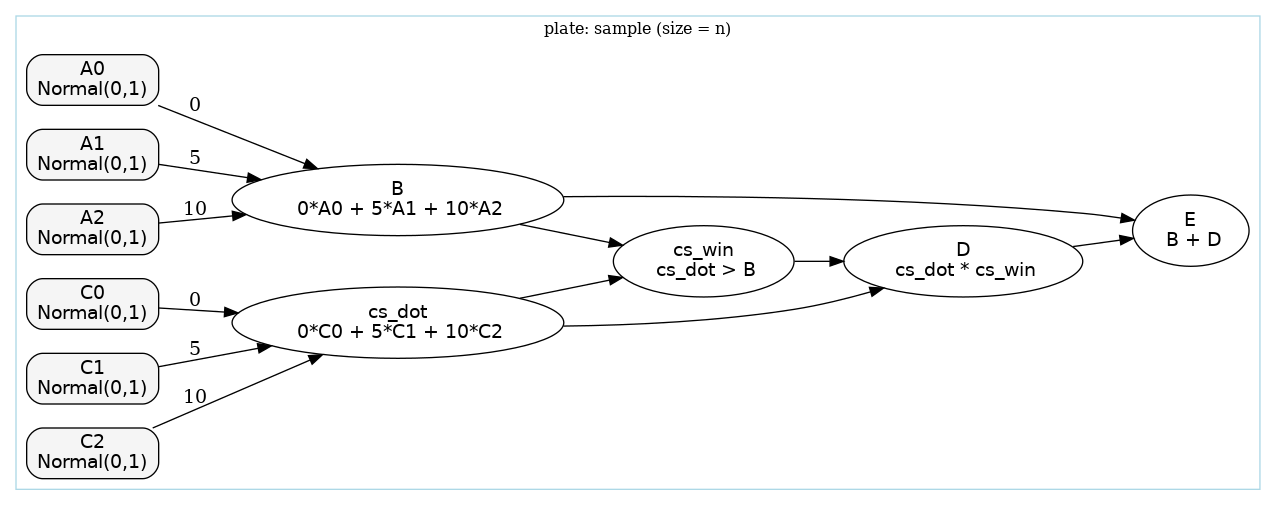
\includegraphics[width= 11cm]{figures/synthetic_causal_model.png}
\caption{Synthetic model involving overdetermination and undercutting used in the evaluation loop.}
\label{fig:synthetic_model}
\end{figure}


\begin{figure}
    \centering
    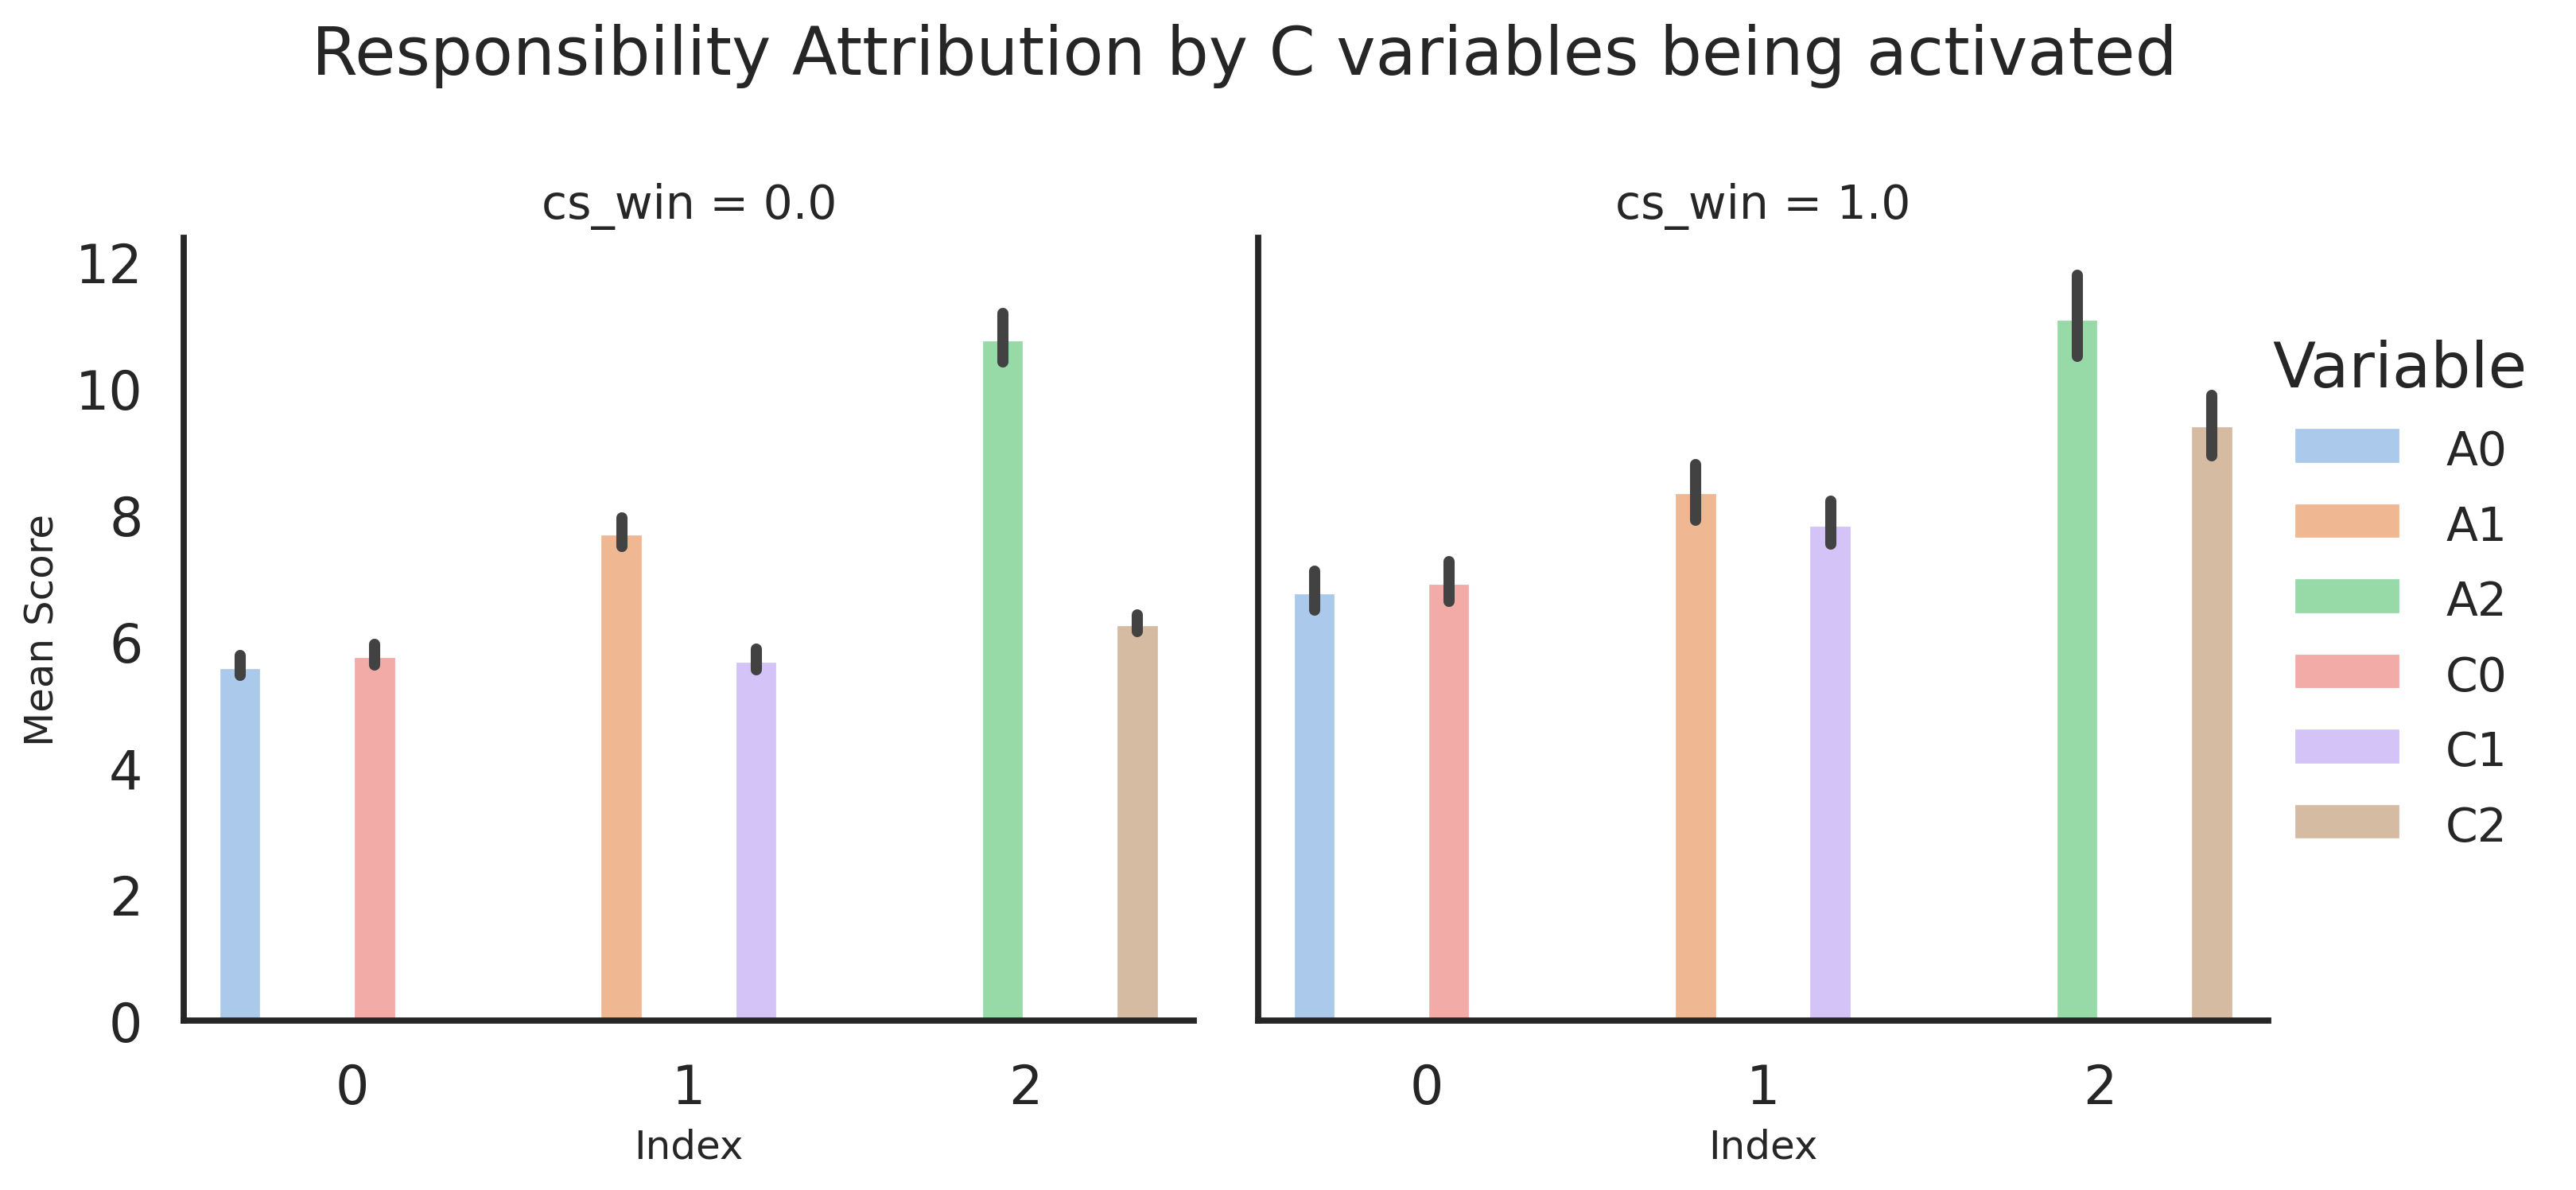
\includegraphics[width=0.9\linewidth]{figures/synthetic_causal_model_responsibility_attribution.png}
    \caption{Mean attribution scores to all upstream features in the synthetic model, 500 individual explanations, all based on a single search sample of size 5000. When `cs\_win=0', the $C$ variables are not activated, and so we expect total scores for all of them to be similar (red, violet, dark brown on the left-hand side). We still expect the scores for $A0$, $A1$, and $A2$ generally to increase independently of what happens with the $C$ variables, which we see on both sides (blue, light brown, and green on both sides). We also expect the scores for $C$ variables to increase if they are activated (red, violet, dark brown on the right-hand side). These expectations are satisfied.}
    \label{fig:synthetic_attribution}
\end{figure}


\begin{figure}
    \centering
    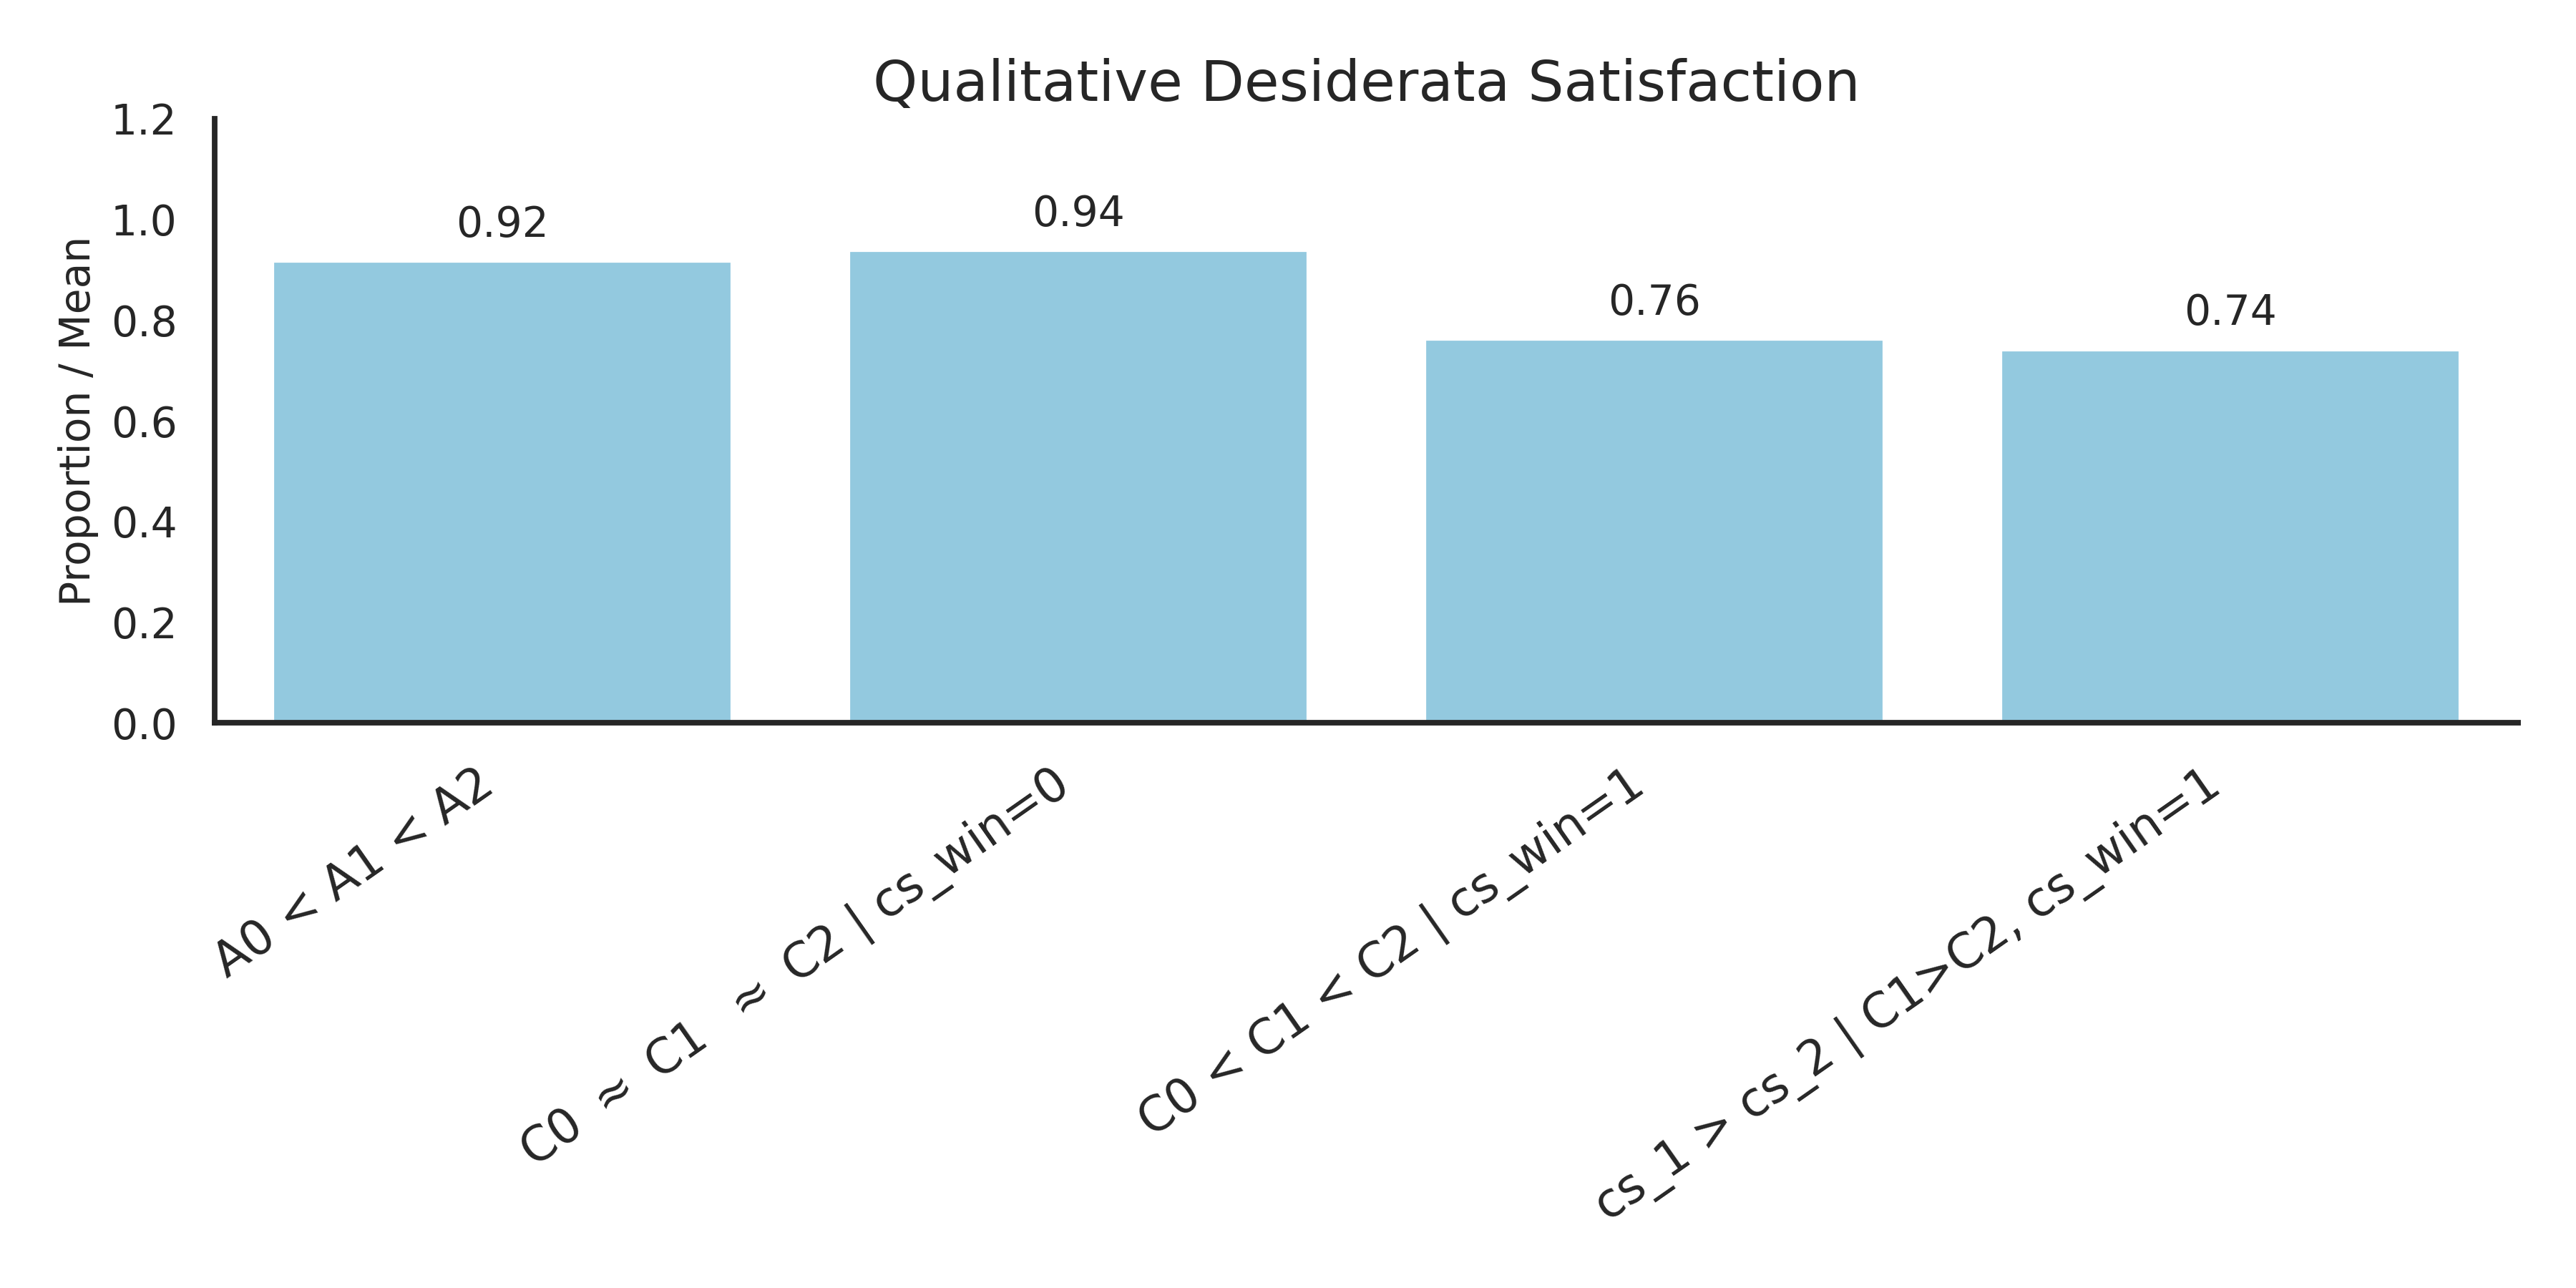
\includegraphics[width=0.9\linewidth]{figures/synthetic_causal_model_summary.png}
    \caption{Qualitative claims satisfaction frequency for causal attribution in the synthetic model, 500 local explanations all based on a single search sample of size 5000. Most of the time, the ordering of the scores for $A$ variables agrees with the ordering of the coefficients. Most of the time, close proximity of scores for inactive $C$ variables is quite high; most often, the ordering for active $C$ variables agrees with the ordering of the coefficients. We do not, however, want an explanation to track coefficients only, which, for instance, is illustrated by the last statement: if scores are reversed, this is mostly due to the disparate direction of the difference between the variable values.}
    \label{fig:synthetic_summary}
\end{figure}

\section{Comparison to Differential Causal Effect}\label{sec:DCE}

This appendix details the Differential Causal Effect comparison summarised in \cref{sec:evaluation}.

Having tested \ourapproach against ground truth in
\cref{sub:synthetic}, we now compare it with gradient-based
attribution on a continuous-input credit-limit example.

A natural baseline for continuous-input attribution is to read causal influence off
the gradient of an interventional mean function. The motivation is direct:
$\mathbb{E}\!\bigl[Y\mid do(X{=}1)\bigr]-\mathbb{E}\!\bigl[Y\mid do(X{=}0)\bigr]$
is the binary ATE, and for a continuous cause one ``arrives at derivative
calculus'' \citep[Section~7.4.3]{ness2025causal} by letting the contrast shrink:
$\partial_x\,\mathbb{E}\!\bigl[Y\mid do(X{=}x)\bigr]$. Generalised to a vector
$\mathbf{x}=(x_1,\ldots,x_d)$ with interventional mean
$m(\mathbf{x})=\mathbb{E}\!\bigl[Y_{\mathbf{X}=\mathbf{x}}\bigr]$, the
\emph{causal gradient} is
\[
\nabla_{\mathbf{x}}\,m(\mathbf{x})
=\Bigl(\partial_{x_1}\mathbb{E}\!\bigl[Y_{\mathbf{X}=\mathbf{x}}\bigr],\;\ldots,\;
        \partial_{x_d}\mathbb{E}\!\bigl[Y_{\mathbf{X}=\mathbf{x}}\bigr]\Bigr),
\]
and each partial is the \emph{differential causal effect} (DCE) of a single
variable at $\mathbf{x}$. \citet{butler2022differential} introduced this
quantity in the Gaussian Process regression setting, where, with the posterior
expected mean expressible as $\sum_n k(x,x^{(n)})\alpha_n$, the DCE has the
closed form $\partial_{x_i}\hat{F}=\sum_n \partial_{x_i}k(x,x^{(n)})\alpha_n$.

\ourapproach and DCE are not direct competitors (DCE estimates a rate of
change, \ourapproach estimates individual-level responsibility), but
\ourapproach inherits the territory of continuous attribution, so a contrast
on a single example is informative. We highlight the differences:
\begin{enumerate}
\item DCE requires $y=F(\mathbf{X},\epsilon)$ with $F$ differentiable;
  \ourapproach requires only that the causal model be sampleable, and the
  inference algorithm for the expanded model is the user's choice (we use Monte
  Carlo throughout).
\item DCE inherits the units of both $\mathbf{X}$ and $Y$, so cross-feature
  comparison is unit-sensitive. The \ourapproach score integrates over the
  necessity- and sufficiency-world densities, so changes to input scale leave
  the score essentially unchanged.\footnote{This unit-invariance is contingent
  on how the alternative-value distribution $\Delta$ is specified. The
  $\epsilon$-excised $\Delta$ of Section~\ref{sec:causal_impact} is invariant to
  a reparameterisation of the input scale precisely when $\epsilon$ is fixed by
  the \emph{probability mass} excised around the factual value (equivalently, in
  standardised units), as in the ROPE/effect-size reading given there, rather
  than as an absolute distance in the raw units of $\mathbf{X}$: an
  absolute-distance $\epsilon$ held fixed across a rescaling would itself become
  unit-dependent and reintroduce the very sensitivity PCI otherwise avoids.}
\item DCE varies abruptly with the local geometry of $F$. The \ourapproach
  score depends on where the factual value sits relative to the
  necessity/sufficiency densities and is therefore non-zero in flat regions
  while remaining locally informative.
\end{enumerate}

\begin{example}[credit-limit assignment]\label{ex:age}
We model an applicant's approved credit limit as a function of \emph{age} and
the \emph{time of application}. The deterministic component is a sigmoidal
rise in age with a small sinusoidal modulation in time-of-day; intuitively,
age should dominate. We consider four settings on two axes: time measured in
hours vs.\ minutes (a units rescaling that should not affect attribution), and
an age prior centred at $30$ vs.\ $40$ (a genuine change in what counts as
unusual). The deterministic component is shown in
Figure~\ref{fig:internal}. Computational details and code are in
\texttt{docs/source/gradient\_based\_attribution.ipynb}.
\end{example}

\begin{figure}[t]
    \centering
    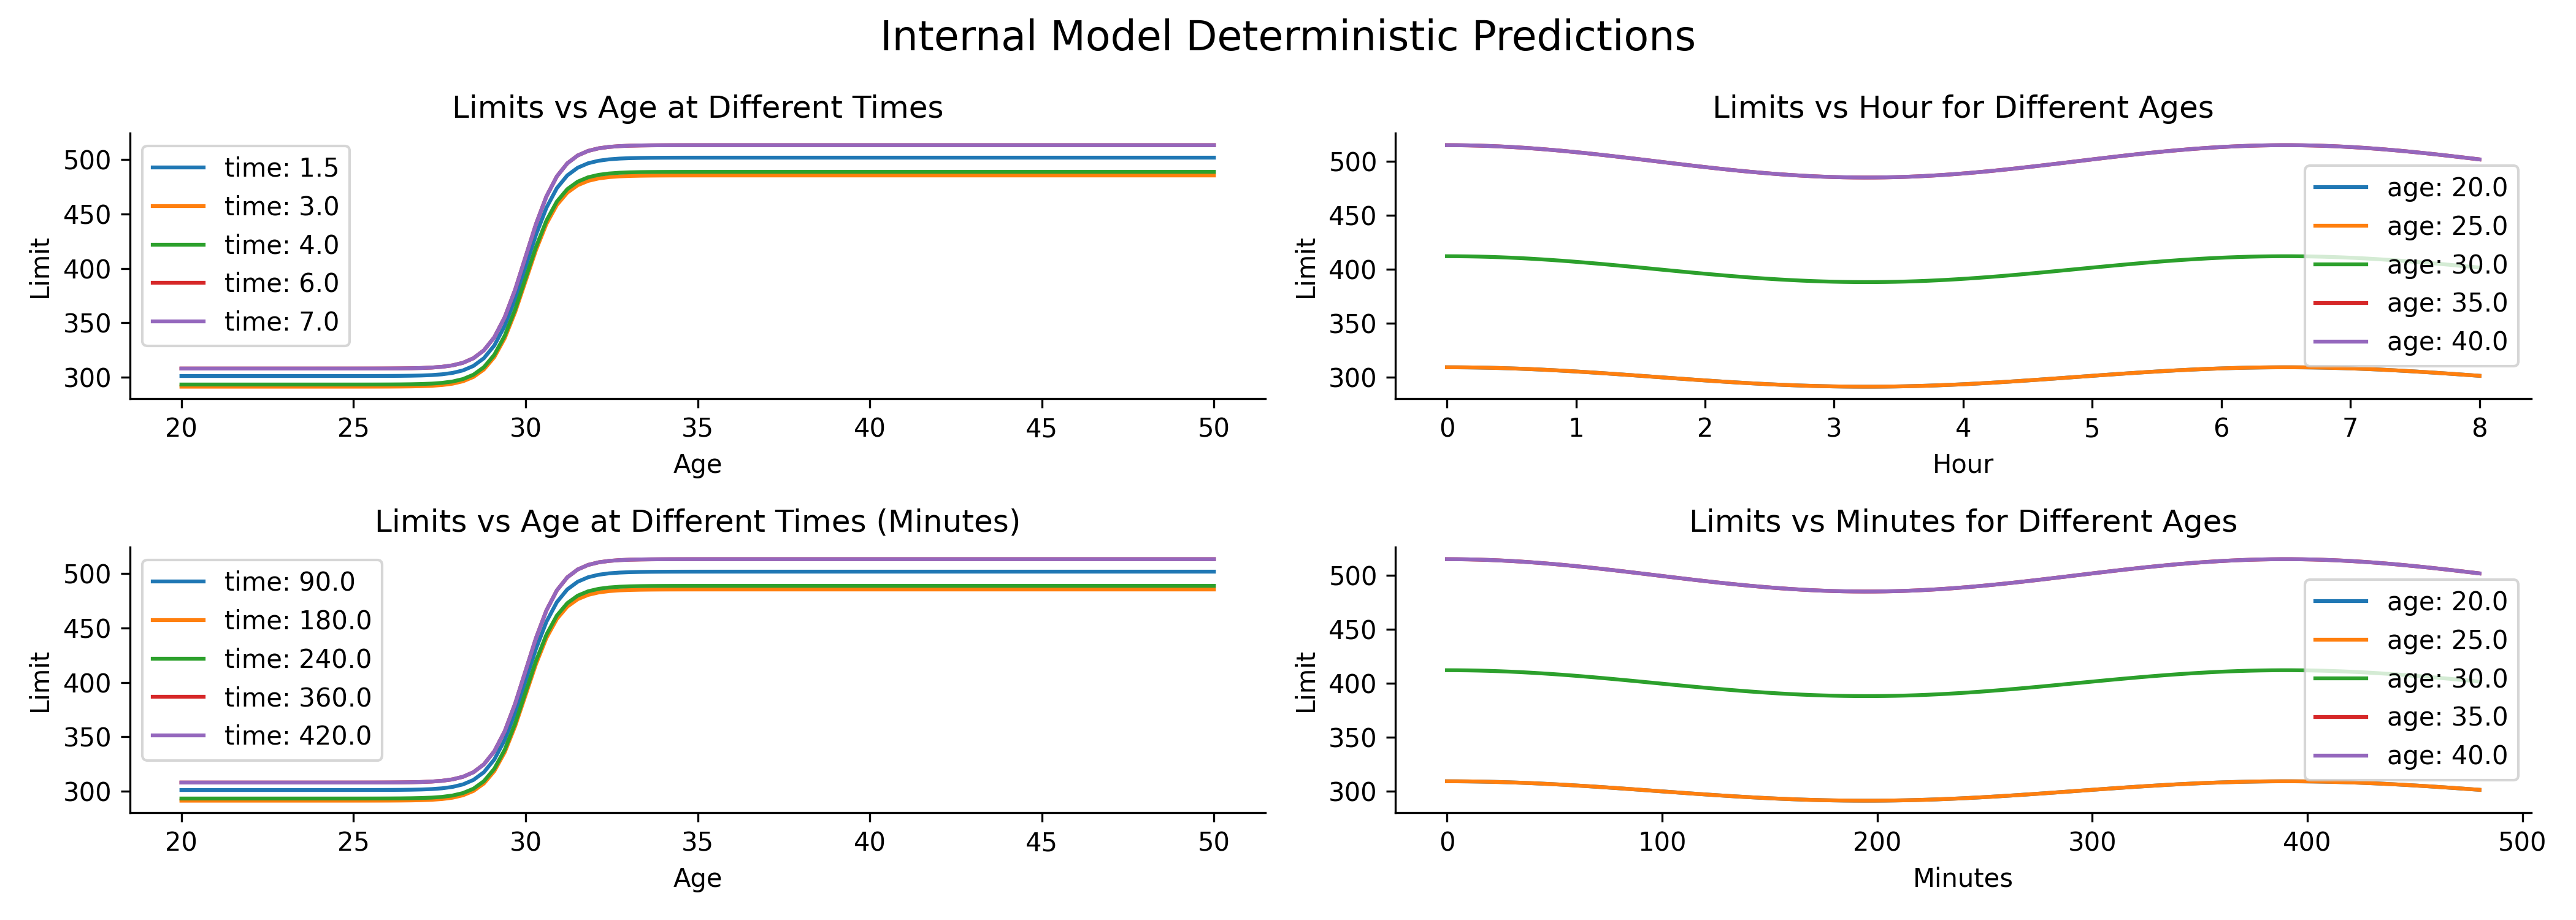
\includegraphics[width=\linewidth]{figures/internal_model_predictions.png}
    \caption{Deterministic component of the credit-limit model
    (Example~\ref{ex:age}), on the hours scale: limit vs.\ age at several times
    of day (left) and limit vs.\ time of day at several ages (right). Age
    dominates the limit, with a small sinusoidal modulation from time of day;
    the minute scale is identical modulo a linear reparameterisation (verified
    in the notebook).}\label{fig:internal}
\end{figure}

\paragraph{\ourapproach scores.} We instantiate $ci$ as the absolute-difference
score from Example~\ref{ex:absolute_score}, $ci(y^s,y^n,y^\star)=|y^n-y^\star|-|y^s-y^\star|$,
and run the search of Section~\ref{sec:causal_impact} on each setting,
conditioning on age and on time of application as singleton suspects.
Figure~\ref{fig:mechanism} shows the mechanism for the canonical setting
(age-$30$ prior, hours): when age is the active suspect the necessity-world
outcome tracks the deterministic curve while the sufficiency-world outcome
stays near factual, and the same picture, with a smaller displacement, holds
for time of application. Table~\ref{tab:dce_means} reports the mean total
scores across all four settings. Two patterns stand out. First, age outscores
time of application in every setting, by roughly a factor of $3/2$, matching the
intuition that the age sigmoid moves the outcome by a much larger absolute
amount than the daily modulation does. Second, the scores are essentially
unchanged between the hours and minutes columns, confirming the unit-invariance
discussed above, whereas the shift from the age-$30$ to the age-$40$ prior
raises every score, since a more unusual factual age means a larger search-space
displacement.

\begin{figure}[t]
    \centering
    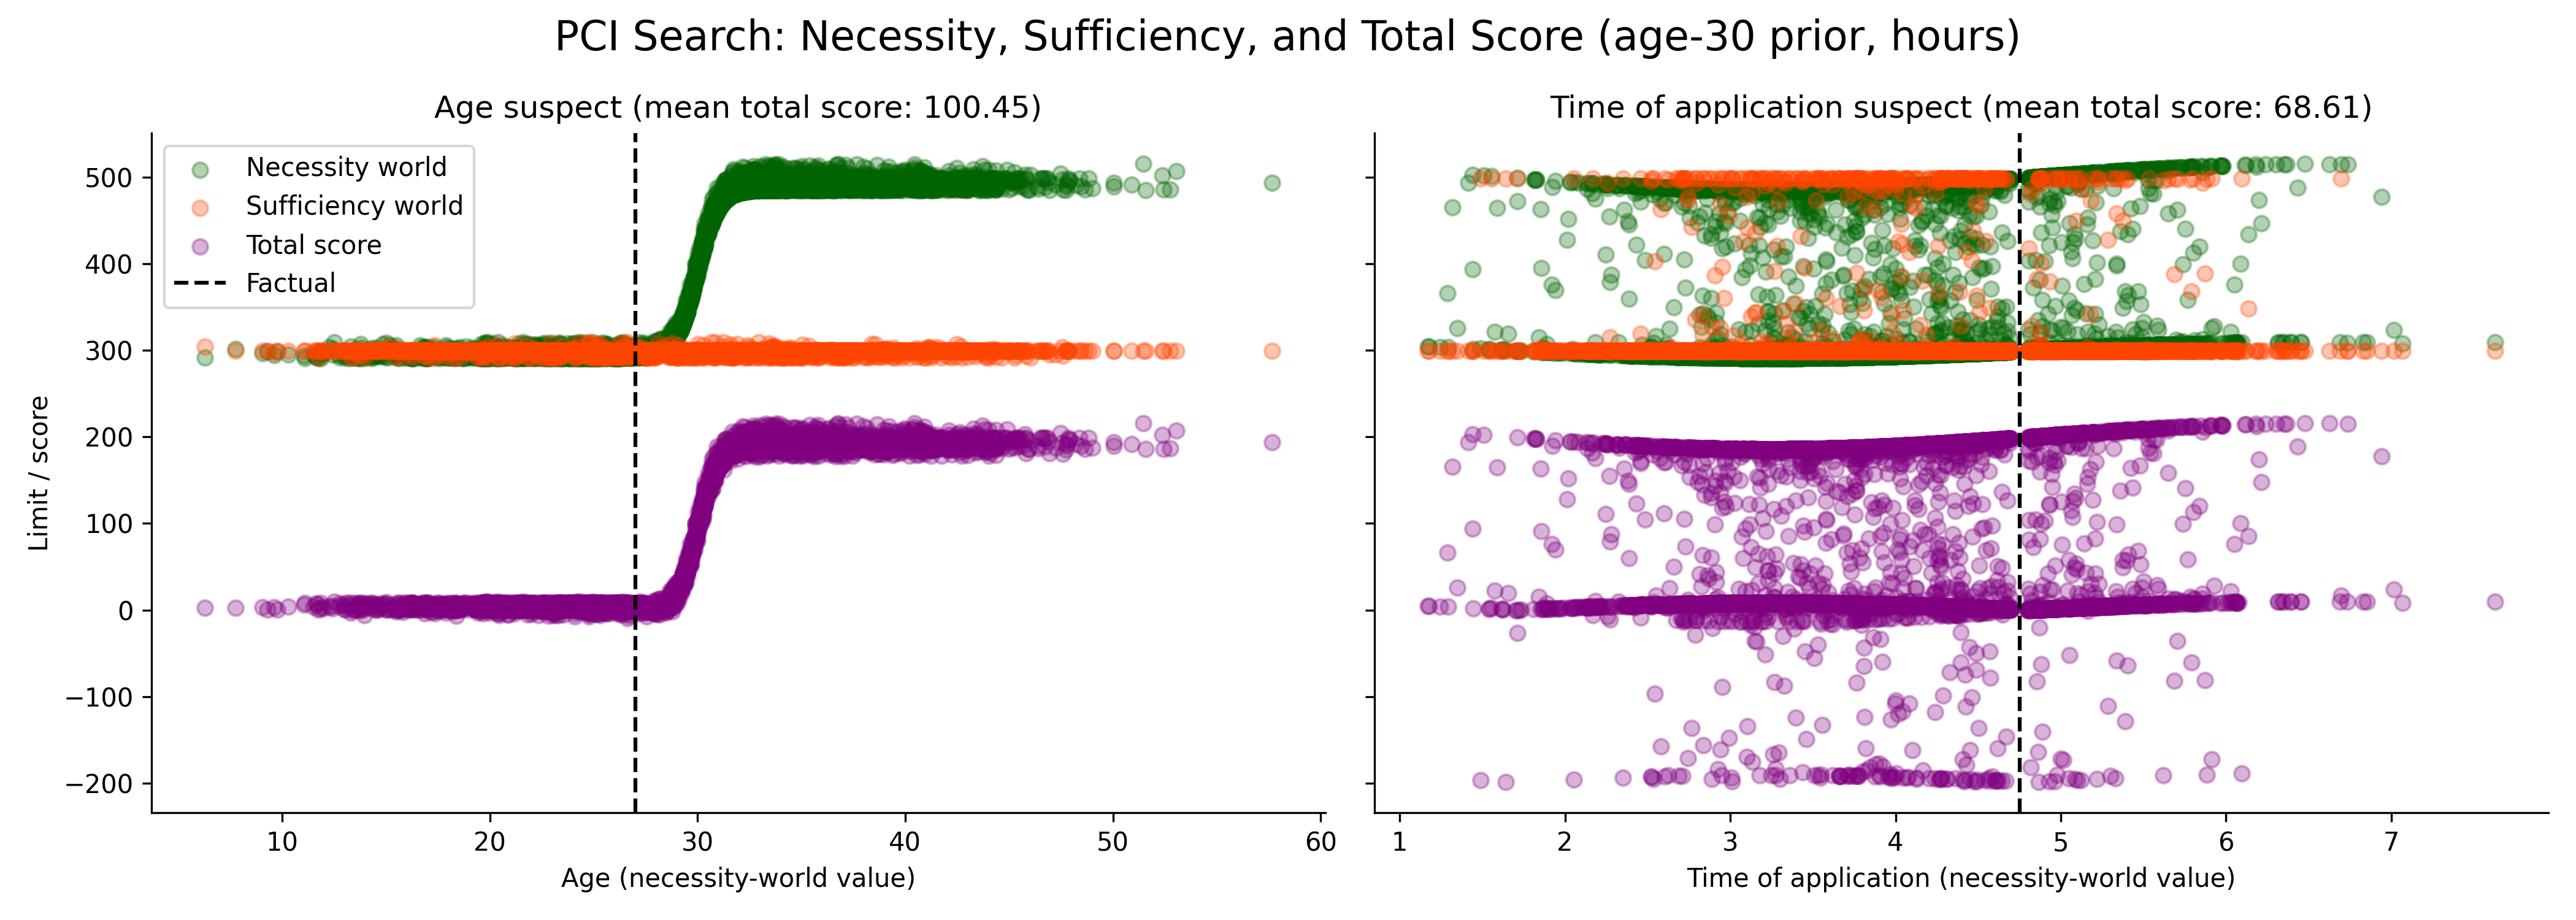
\includegraphics[width=\linewidth]{figures/search_samples_combined.png}
    \caption{PCI search for the canonical setting (age-$30$ prior, hours), with
    age (left) and time of application (right) as the active suspect.
    Necessity-world (green) and sufficiency-world (orange) limit samples and the
    total score (purple) are plotted against the necessity-world value of the
    suspect; the dashed line marks the factual. The necessity world departs from
    factual along the deterministic response while the sufficiency world stays
    near it; each panel title gives the mean total score.}\label{fig:mechanism}
\end{figure}

\begin{table}[t]
\centering
\caption{Mean \ourapproach total scores for age and time of application across
the four settings (time unit $\times$ age prior), at the factual instance. Age
outscores time in every setting; the hours and minutes columns agree
(unit-invariance), while the age-$40$ prior raises all scores relative to
age-$30$ (a more unusual factual age).}
\label{tab:dce_means}
\vspace{4pt}
\begin{tabular}{l cc cc}
\toprule
& \multicolumn{2}{c}{age-$30$ prior} & \multicolumn{2}{c}{age-$40$ prior} \\
\cmidrule(lr){2-3}\cmidrule(lr){4-5}
Suspect & hours & minutes & hours & minutes \\
\midrule
Age                  & $100.45$ & $97.95$  & $177.87$ & $176.56$ \\
Time of application  & $68.61$  & $66.51$  & $117.97$ & $118.42$ \\
\bottomrule
\end{tabular}
\end{table}

\paragraph{PCI vs.\ DCE across the input grid.}
Figure~\ref{fig:contrast} contrasts the two methods on the same grid of factual
values (age-$30$ prior, hours); the other three settings give qualitatively the
same picture. The top panel plots the difference between the \ourapproach scores
for age and for time of application: it is positive everywhere, so age is
consistently the more responsible variable, with the gap largest near the steep
region of the age-limit sigmoid and growing for ages further from the prior
mean. The bottom panels show the DCE for the two inputs, and two differences
with \ourapproach stand out. First, on the hour scale the DCE for time of
application exceeds the DCE for age over most of the grid and traces a visible
sine wave, whereas \ourapproach reports age as the more responsible variable
everywhere. Second, switching the time unit from hours to minutes flattens the
time DCE by roughly a factor of $60$, making the unit sensitivity explicit. Both
are direct consequences of DCE's role as a rate-of-change estimator rather than
a responsibility score, and both make it harder to compare across features and
across reparameterisations.

\begin{figure}[t]
    \centering
    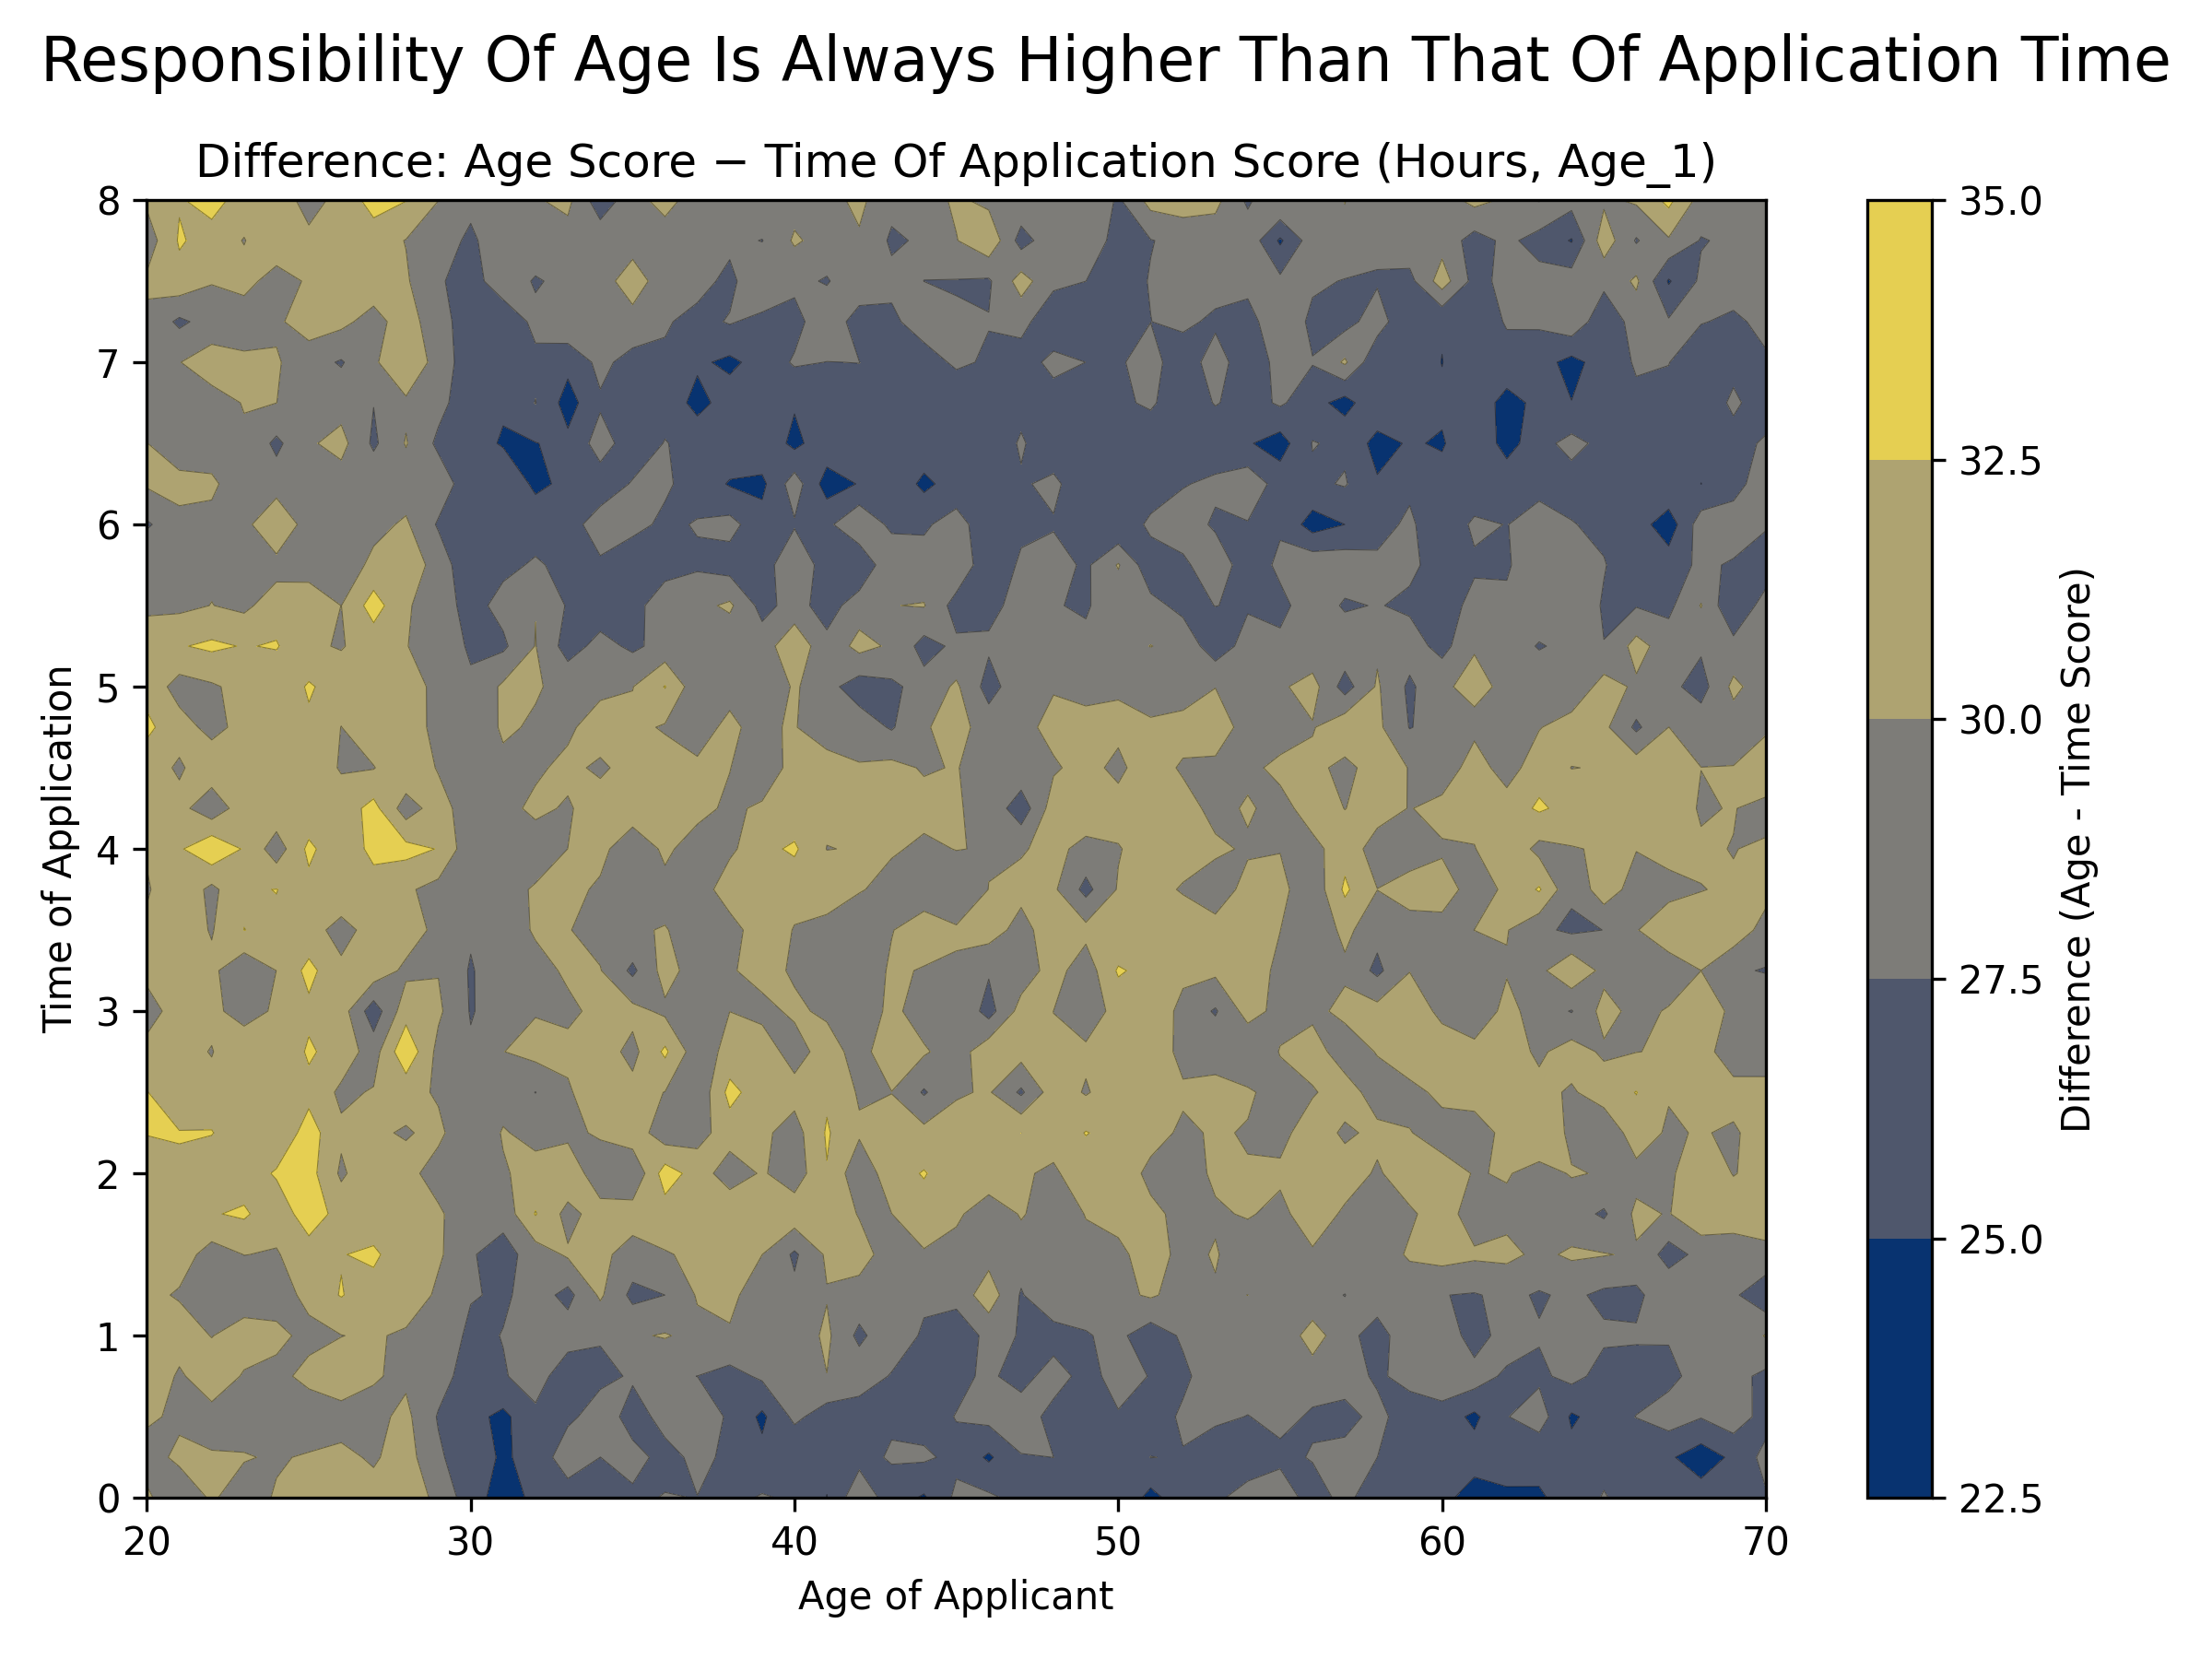
\includegraphics[width=0.62\linewidth]{figures/contour_diff_hours_age_1.png}\\[6pt]
    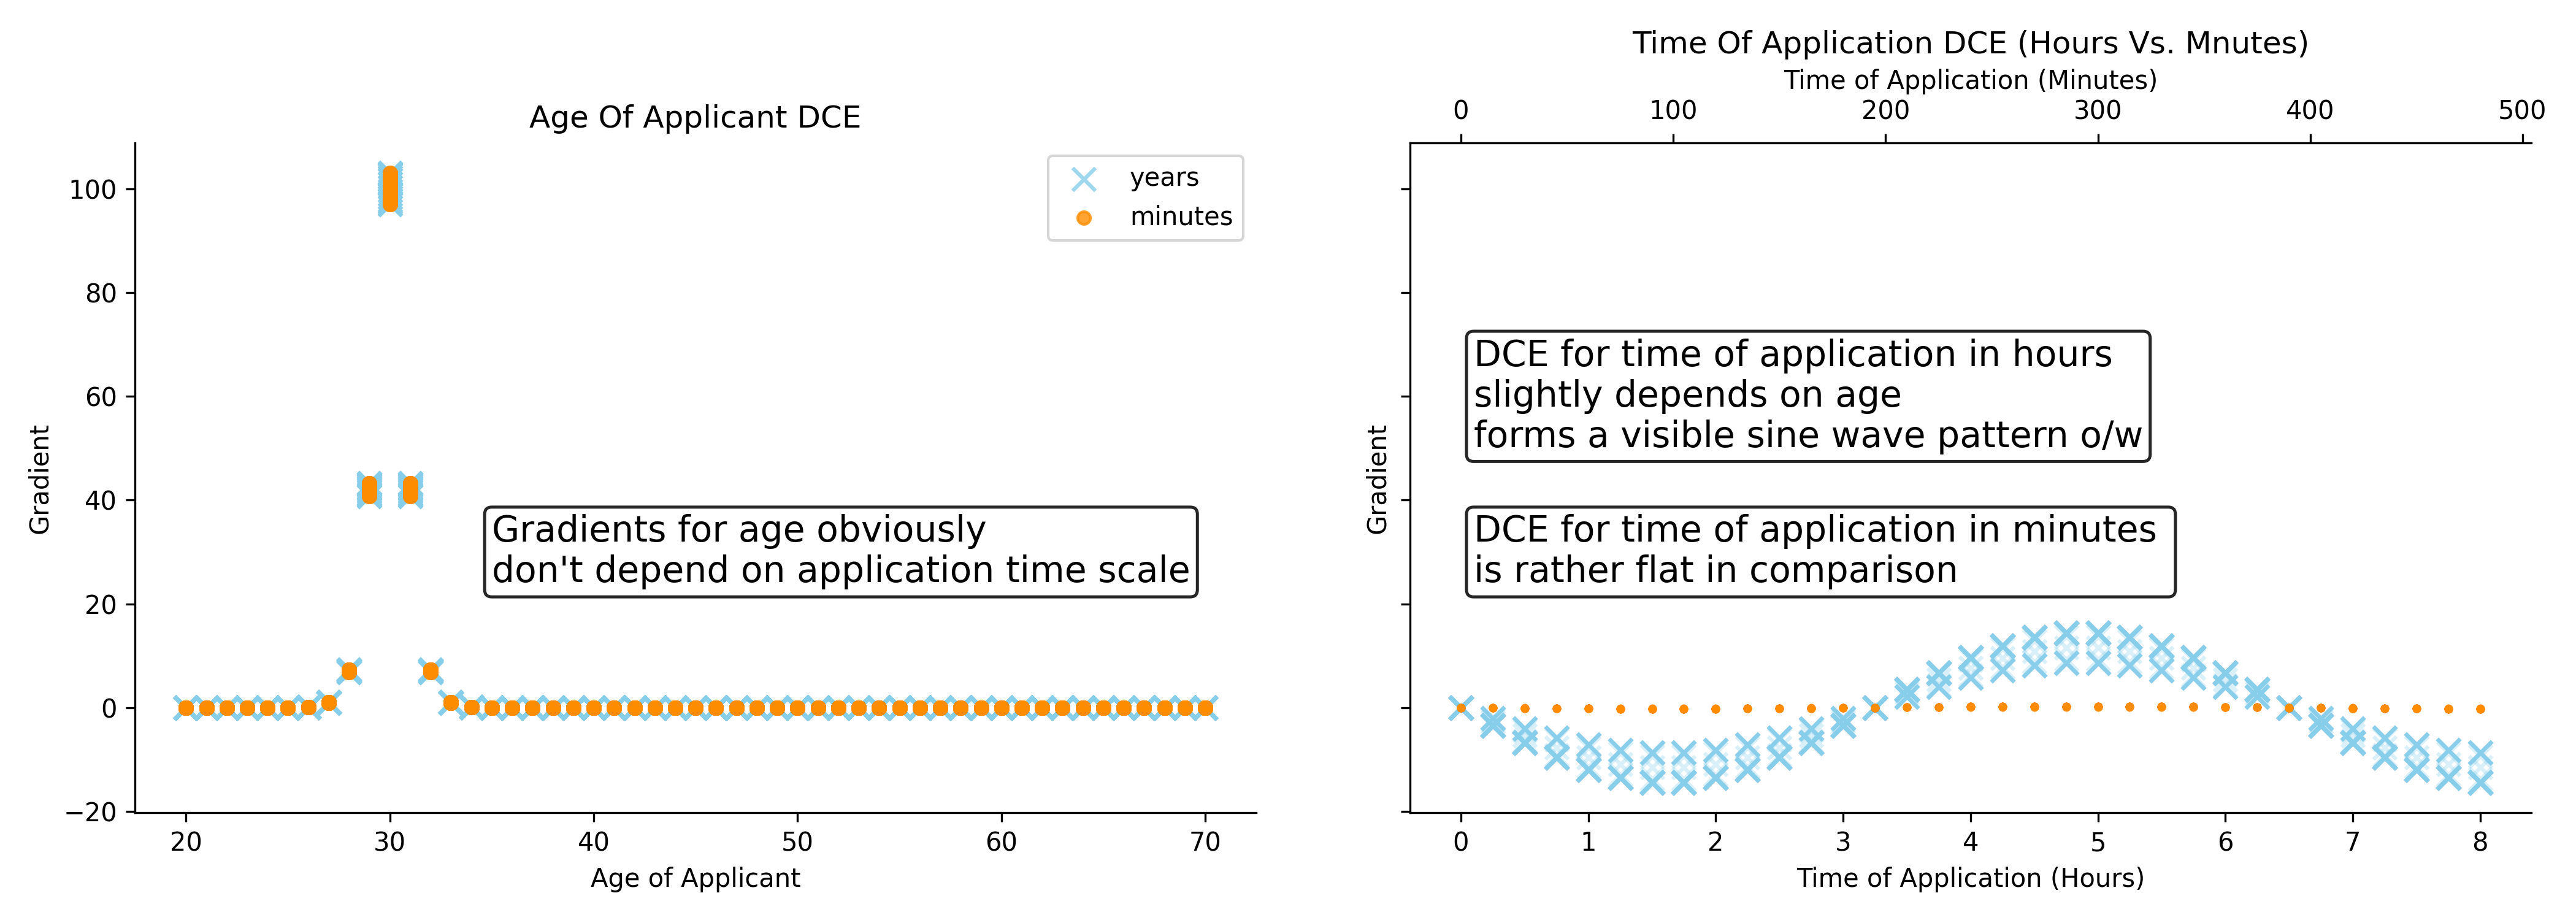
\includegraphics[width=\linewidth]{figures/dce_age_time_hours_minutes.png}
    \caption{\textbf{PCI vs.\ DCE on the credit-limit grid} (age-$30$ prior,
    hours). \emph{Top:} difference between the \ourapproach scores for age and
    for time of application; positive everywhere, largest near the steep region
    of the age-limit sigmoid and for ages far from the prior mean, so age is
    always the more responsible variable. \emph{Bottom:} DCE for age (left) and
    time of application (right) on both unit scales. Age has the larger absolute
    DCE only inside the narrow steep region of the sigmoid; elsewhere time of
    application dominates on the hour scale and goes comparatively flat on the
    minute scale, illustrating DCE's shape and unit sensitivity.}
    \label{fig:contrast}
\end{figure}

\FloatBarrier  % keep the DCE figures within this appendix, not the next

\section{Relation with Actual Causality} \label{sec:relation_with_ac}

 Sections~\ref{sec:shap_examples}--\ref{sec:DCE} have
positioned \ourapproach against feature-attribution baselines. We now turn to
\ourapproach's relation to the causal-attribution tradition it inherits the
witness mechanism from --- Halpern's actual causality. This section establishes
the \emph{formal} connection (Theorems~\ref{th:ac-exp}--\ref{th:exp-ac} and
Proposition~\ref{prop:filter}); Section~\ref{sub:pearl_actual_cause_prob} adds
the side-by-side comparison with Pearl's \emph{probability of actual
causation}; and Section~\ref{sec:ac_benchmark} measures the empirical gap in
runtime and verdict recovery.

\ourapproach{} is not meant to explicate Halpern's notion of actual causality; the goal
is to combine the intuitions underlying Halpern's notion with those motivating Pearl's
probabilities of necessity and sufficiency to provide a more general tool for causal
attribution. Nevertheless, to show that we preserve the spirit of Halpern's definition,
we now record the connection between actual causality and the joint necessity-sufficiency
machinery of Section~\ref{sec:causal_impact}. The goal is to show that there is a
natural choice of variable selection distribution $\Gamma$ and alternative-value
distribution $\Delta$ under which \ourapproach{} verdicts agree with actual-causality
verdicts. With one caveat: probability-of-causation maximisation will not identify
subset-minimal causes that are not cardinality-minimal, a misalignment we
characterise and remedy below.

\medskip\noindent\textit{Scope: a necessity-only correspondence.} Halpern's definition
involves factivity, context-sensitive necessity, and minimality, but no sufficiency
clause analogous to Pearl's $\mathrm{PS}$ or $\mathrm{PNS}$. The correspondence we
establish in this section is therefore \emph{necessity-only}: the sufficiency component
of the kernel $\Phi$ defined below acts as a factivity check (restoring factual values
must preserve $\varphi$ under fixed noise), not as a substantive sufficiency-attribution
component. The substantive sufficiency component of \ourapproach{}, the $Y^s$ factor
in Definition~\ref{def:jointnecsuf} and the $ci_S$ term in
Section~\ref{sub:synthetic}, is exercised in the synthetic overdetermination and
undercutting evaluation (Section~\ref{sub:synthetic}), the differential causal effect
comparison (Section~\ref{sec:DCE}), and the SIR benchmark
(Section~\ref{sec:sir_benchmark}), all of which are settings where AC cannot adjudicate.
The narrowness of this section's correspondence reflects what AC itself permits, not a
limitation of \ourapproach{}.

We first recall Halpern's definition.

\begin{definition}[Actual Cause, after \citealp{actualCausalityHalpern}] \label{def:ac}
    \(\mathbf{C} = \mathbf{c}\) is an actual cause of \(\varphi\) in the causal setting \((M, \mathbf{u})\) if the following three conditions hold:
    \begin{itemize}
        \item \textbf{Factivity}: \((M, \mathbf{u}) \vDash (\mathbf{C} = \mathbf{c}\,)\) and \((M, \mathbf{u}) \vDash \varphi\),
        \item \textbf{Context-sensitive Necessity}: There is a set of variables \(\mathbf{T} \subseteq \mathbf{V}\) and an alternative setting \(\mathbf{c'}\) of variables in \(\mathbf{C}\) such that if \((M, \mathbf{u}) \vDash \mathbf{T} = \mathbf{t^\star}\), then
            \[(M, \mathbf{u}) \vDash [\mathbf{C} \leftarrow \mathbf{c'}, \mathbf{T} \leftarrow \mathbf{t^\star}] \neg \varphi,\]
        \item \textbf{Minimality}: \(\mathbf{C}\) is minimal; there is no strict subset \(\mathbf{C_{sub}} \subset \mathbf{C}\) such that \(\mathbf{C_{sub}} = \mathbf{c_{sub}}\) satisfies the above two conditions where $\mathbf{c_{sub}}$ is the restriction of \(\mathbf{c}\) to the variables in \(\mathbf{C_{sub}}\).
        \end{itemize}
\end{definition}

\noindent To connect this to \ourapproach{}, we instantiate the joint
necessity-sufficiency machinery (Definition~\ref{def:jointnecsuf}) at a single
configuration $(\mathbf{C}, \mathbf{T})$ and a fixed noise realisation $\mathbf{u}$,
and read off the configuration-level contribution. The resulting kernel combines the
same three ingredients as Halpern's definition: a sufficiency check at factual values,
a necessity check against alternatives, and a $\Gamma$-weight that records how much
the configuration is being asked about.

\begin{definition}[AC-aligned PCI kernel] \label{def:ackernel}
Fix a PSCM $M=\langle\mathbf{U},\mathbf{V},\mathbf{F},P_{\mathbf{U}}\rangle$,\footnote{%
The kernel and the theorems below take the full PSCM (structural equations $\mathbf{F}$
plus noise distribution $P_{\mathbf{U}}$) as given, since both the sufficiency and the
necessity factors require sampling counterfactual outcomes under $\mathbf{u}$. As
discussed in Section~\ref{sec:intro}, this is a stronger commitment than approaches
that bound $\mathrm{PN}/\mathrm{PS}/\mathrm{PNS}$ from observational data and a causal
graph alone, but is the price of pointwise (not just bound) verdicts at the
configuration level.} a noise
realisation $\mathbf{u}$, suspect and witness sets $\mathbf{S},\mathbf{W}\subseteq\mathbf{V}$
with factual values $\mathbf{s}^\star,\mathbf{w}^\star$, a variable selection
distribution $\Gamma$ on $2^{\mathbf{S}}\times 2^{\mathbf{W}}$ with mass function
$p^\Gamma$, and an alternative-value distribution $\Delta(\mathbf{s}^\star)$. For an
outcome event $\varphi$, active suspect set $\mathbf{C}\subseteq\mathbf{S}$ and active
witness set $\mathbf{T}\subseteq\mathbf{W}$ with $\mathbf{T}\cap\mathbf{C}=\emptyset$,
define
\begin{align}
\Phi(\mathbf{C},\mathbf{T})
&\;:=\;
p^\Gamma(\mathbf{C},\mathbf{T})
\;\cdot\;
\mathbb{I}\!\left[(M,\mathbf{u})\vDash
[\mathbf{C}\!\leftarrow\!\mathbf{s}^\star\!\mid_{\mathbf{C}},\,
 \mathbf{T}\!\leftarrow\!\mathbf{w}^\star\!\mid_{\mathbf{T}}]\,\varphi\right]
\nonumber \\
&\quad\;\cdot\;
\int
\mathbb{I}\!\left[(M,\mathbf{u})\vDash
[\mathbf{C}\!\leftarrow\!\mathbf{c}',\,
 \mathbf{T}\!\leftarrow\!\mathbf{w}^\star\!\mid_{\mathbf{T}}]\,\neg\varphi\right]
\Delta_{\mathbf{C}}(\mathbf{s}^\star)(d\mathbf{c}').
\label{eq:ackernel}
\end{align}
\end{definition}

\medskip\noindent Concretely, $\Phi(\mathbf{C},\mathbf{T})$ is the
matched-configuration slice of the joint necessity-sufficiency measure $P_k^{s,n}$
from Definition~\ref{def:jointnecsuf}: integration over $P_{\mathbf{U}}$ is replaced
by point evaluation at $\mathbf{u}$, and both the sufficiency and the necessity sums
are pinned to the same $(\mathbf{C},\mathbf{T})$ pair, mirroring AC's structure of
testing factivity and the alternative against a single suspect/witness pair. The
kernel is positive exactly when three conditions hold simultaneously:
$(\mathbf{C},\mathbf{T})$ has positive $\Gamma$-mass; restoring $\mathbf{C}$ to its
factual values while holding $\mathbf{T}$ fixed preserves $\varphi$ under $\mathbf{u}$
(the factivity-as-sufficiency component); and there exists a
$\Delta$-positive-density alternative $\mathbf{c}'$ for which the corresponding
intervention overturns $\varphi$ under $\mathbf{u}$ (the necessity component). The
first factor takes the role played by the suspect/witness biases $b_s,b_w$ in earlier
work: regularity of $\Gamma$ --- positive $p^\Gamma$ on every legal configuration
--- corresponds to the old $-0.5<b_s,b_w<0.5$ regularity. We will say that $\Gamma$
is \emph{regular} when $p^\Gamma(\mathbf{C}',\mathbf{T}')>0$ for every
$(\mathbf{C}',\mathbf{T}')$ with $\mathbf{C}'\subseteq\mathbf{S}$,
$\mathbf{T}'\subseteq\mathbf{W}$, $\mathbf{C}'\cap\mathbf{T}'=\emptyset$.

We can now record the forward direction.

\begin{theorem}\label{th:ac-exp}
    Suppose that $\mathbf{C}$ is an actual cause of $\varphi$ with witness set $\mathbf{T}$ in $(M,\mathbf{u})$. Take any $\{\mathbf{S}=\mathbf{s}\}\supseteq\mathbf{C}$ as the potential cause set, subject to the constraint that no element of $\mathbf{S}$ is a deterministic function (under $M$) of any subset of the remaining elements of $\mathbf{S}$,\footnote{Equivalently, $\mathbf{S}$ is closed under no nontrivial structural equation of $M$. The constraint excludes admitting both $S$ and a deterministic descendant $H=f(S,\ldots)$ as candidates in the same suspect set, but covers all candidate sets standardly considered in the AC literature, where structural descendants of one candidate are not admitted as separate candidates: their contribution is mediated by the equation, and AC's minimality clause already prefers the ancestor alone. The same closure condition discharges a joint-support concern: the next assumption requires $\Delta(\mathbf{s})$ to place positive density on every \emph{joint} alternative configuration $\mathbf{s}'\in\dom(\mathbf{S})\setminus\{\mathbf{s}\}$, not merely positive marginal density on each component. In a chain $S\to H$ with $H=f(S)$, joint assignments such as $(S{=}0, H{=}1)$ are impossible under the structural equations, so any $\Delta$ that placed mass on them would be incompatible with $M$. Closure rules out exactly this case: when no element of $\mathbf{S}$ is a deterministic function of the remaining elements, the joint domain $\dom(\mathbf{S})$ contains no rectangles forced to zero measure by $M$, and a $\Delta$ with positive PMF or Lebesgue density on every $\mathbf{s}'\neq\mathbf{s}$ is consistent with $M$ on the suspect set. In the stone-throwing benchmark of Section~\ref{sec:ac_benchmark}, the suspect set is $\{A_i,B_i\}_i$ and the deterministic mediators $\{W^a_i,W^b_i\}_i$ live in the witness set, not the suspect set, exactly to keep the suspect set closure-respecting. Witnesses are pinned at their factual values and are not subject to a joint-support requirement on alternatives, so they need no analogous condition.} and any $\mathbf{W}\supseteq\mathbf{T}$ as the potential witness set. Assume $\Gamma$ is regular and that $\Delta(\mathbf{s})$ assigns positive density to every $\mathbf{s}'\in\dom(\mathbf{S})\setminus\{\mathbf{s}\}$ (positive PMF in the discrete case, positive Lebesgue density in the continuous case). In the continuous case, assume additionally:
    \begin{itemize}
    \item[(i)] the structural equations of $M$ downstream of $\mathbf{C}$ are continuous in
    $\mathbf{c}'$ under fixed $\mathbf{u}$;
    \item[(ii)] $\neg\varphi$ is open in $\dom(Y)$ (or, more weakly, the boundary of
    $\neg\varphi$ has measure zero under the pushforward of $Y$).
    \end{itemize}
    Then
    \begin{align}
    \Phi(\mathbf{C},\mathbf{T}) > 0,
    \label{eq:pect}
    \end{align}
    and therefore
    \[
    \sum_{\mathbf{T}'\subseteq\mathbf{W}} \Phi(\mathbf{C},\mathbf{T}')\;>\;0.
    \]
\end{theorem}

\begin{proof}
Fix $\mathbf{u}$, $\mathbf{c}'$, and $\mathbf{T}$ as witnesses to the satisfaction of
the conditions in Definition~\ref{def:ac}. The context-sensitive-necessity clause
forces $\mathbf{T}\cap\mathbf{C}=\emptyset$, since otherwise the joint intervention
$[\mathbf{C}\!\leftarrow\!\mathbf{c}',\,\mathbf{T}\!\leftarrow\!\mathbf{t}^\star]$ would
be ill-defined. It remains to show that each of the three factors in
$\Phi(\mathbf{C},\mathbf{T})$ is strictly positive.
\begin{itemize}
\item \emph{Selection weight.} By regularity of $\Gamma$,
$p^\Gamma(\mathbf{C},\mathbf{T})>0$.
\item \emph{Sufficiency indicator.} With exogenous noise $\mathbf{u}$ held constant,
factivity gives $(M,\mathbf{u})\vDash\varphi$. Restoring $\mathbf{C}$ to
$\mathbf{s}^\star\!\mid_{\mathbf{C}}$ and $\mathbf{T}$ to $\mathbf{w}^\star\!\mid_{\mathbf{T}}$
leaves the model agreeing with $(M,\mathbf{u})$ on every variable, so the indicator
evaluates to $1$.
\item \emph{Necessity integral.} Context-sensitive necessity provides a specific
$\mathbf{c}'$ witnessing
$(M,\mathbf{u})\vDash[\mathbf{C}\!\leftarrow\!\mathbf{c}',\mathbf{T}\!\leftarrow\!\mathbf{t}^\star]\neg\varphi$.
The closure condition on $\mathbf{S}$ and the positive-density assumption on
$\Delta(\mathbf{s})$ imply that $\mathbf{c}'$ lies in the support of
$\Delta_{\mathbf{C}}(\mathbf{s}^\star)$. We treat the two cases separately.
\emph{Discrete case}: the singleton $\{\mathbf{c}'\}$ has positive PMF
$\Delta_{\mathbf{C}}(\{\mathbf{c}'\})>0$ by hypothesis, so the integral is at least
$\Delta_{\mathbf{C}}(\{\mathbf{c}'\})>0$. \emph{Continuous case}: hypothesis~(i) gives
continuity of the intervention map $\mathbf{c}'\mapsto Y$ at fixed $\mathbf{u}$;
hypothesis~(ii) places $Y(\mathbf{c}')$ in the interior of $\neg\varphi$; pulling back
an open neighbourhood within $\neg\varphi$ yields an open neighbourhood of
$\mathbf{c}'$ on which the indicator equals $1$, and this neighbourhood has positive
Lebesgue measure and hence positive $\Delta_{\mathbf{C}}$-mass by the
positive-density hypothesis. In either case the integral is strictly positive.
\end{itemize}
The product of three strictly positive factors is strictly positive, giving
$\Phi(\mathbf{C},\mathbf{T})>0$. Summing over $\mathbf{T}'\subseteq\mathbf{W}$ adds
non-negative terms to a positive one, preserving positivity. The proof uses factivity
and context-sensitive necessity but not minimality: the same conclusion holds whenever
$\mathbf{C}$ satisfies factivity and context-sensitive necessity in $(M,\mathbf{u})$,
a fact we will use in Proposition~\ref{prop:filter}.
\end{proof}

\medskip\noindent\textit{Remark (when (i)--(ii) bite).} In settings with continuous
outcomes and an open event such as a threshold $\{Y>y_0\}$ (for instance the SIR
overshoot benchmark of Section~\ref{sec:sir_benchmark}), both hypotheses are
satisfied trivially. Binary-output models, where $Y$ takes values in $\{0,1\}$, satisfy
(ii) automatically (every subset of a discrete codomain is open) but may not satisfy
(i) when the binary output comes from thresholding a continuous score. In such cases
the proof falls back to the discrete branch, which only requires positive PMF on the
witnessing $\mathbf{c}'$.

The opposite direction follows by reading the proof in reverse on the necessity factor.

\begin{theorem}\label{th:exp-ac}
Under the same hypotheses on $\{\mathbf{S}=\mathbf{s}\}$, $\Gamma$, and $\Delta$ as
in Theorem~\ref{th:ac-exp}, if
\[
\sum_{\mathbf{T}'\subseteq\mathbf{W}} \Phi(\mathbf{C},\mathbf{T}')\;>\;0,
\]
then both factivity ($(M,\mathbf{u})\vDash\varphi$) and the
context-sensitive-necessity condition in Definition~\ref{def:ac} hold for
$\mathbf{C}$ in $(M,\mathbf{u})$.
\end{theorem}

\begin{proof}
Since $\Phi$ is non-negative, the assumption forces $\Phi(\mathbf{C},\mathbf{T}')>0$
for at least one $\mathbf{T}'\subseteq\mathbf{W}$. By Definition~\ref{def:ackernel},
each factor of $\Phi(\mathbf{C},\mathbf{T}')$ is strictly positive. The sufficiency
indicator equals $1$, i.e.\
$(M,\mathbf{u})\vDash[\mathbf{C}\!\leftarrow\!\mathbf{s}^\star\!\mid_{\mathbf{C}},\,\mathbf{T}'\!\leftarrow\!\mathbf{w}^\star\!\mid_{\mathbf{T}'}]\varphi$;
since pinning variables to their factual values under fixed $\mathbf{u}$ leaves every
variable unchanged, this is equivalent to $(M,\mathbf{u})\vDash\varphi$, giving
factivity. The necessity integral being positive provides a
$\Delta_{\mathbf{C}}$-positive-density set of values $\mathbf{c}'$ for which
$(M,\mathbf{u})\vDash[\mathbf{C}\!\leftarrow\!\mathbf{c}',\,\mathbf{T}'\!\leftarrow\!\mathbf{w}^\star\!\mid_{\mathbf{T}'}]\neg\varphi$;
any such $\mathbf{c}'$, together with $\mathbf{T}'$, witnesses the existential in the
context-sensitive-necessity clause of Definition~\ref{def:ac}.
\end{proof}

\medskip\noindent\textit{Remark (deterministic intermediates and joint support).}
The hypothesis on $\{\mathbf{S}=\mathbf{s}\}$ is what rules out the following obstruction.
Suppose the suspect set were closed under the structural equations of $M$, e.g., both
Sally's throw $S$ and the bottle's hit $H = f(S,\ldots)$ admitted as candidates. Then the
joint assignment $(S{=}0, H{=}1)$ is structurally impossible, and any alternative-value
distribution consistent with $M$ assigns it density zero, so the joint full-support
condition required to recover the witnessing $\mathbf{c}'$ from $\Phi > 0$ fails.
Restricting suspects to variables that are not deterministic functions of the others
under $M$ removes this obstruction. The constraint is also conservative with respect to
the AC literature: in the canonical stone-throwing setup, the candidate set is
$\{S_{Sally}, S_{Bill}\}$, with $H$ as the outcome rather than a candidate, and AC's own
minimality clause already prefers ancestor candidates over their deterministic descendants
when both are admitted. Sections~\ref{sub:synthetic} and~\ref{sec:ac_benchmark} adopt the
same convention experimentally --- the continuous synthetic benchmark uses the six roots
as suspects and the discrete scaled-throwing benchmark uses $\{A_i,B_i\}_i$ as suspects
with the deterministic mediators $\{W^a_i,W^b_i\}_i$ as witnesses --- in both cases
deterministic intermediates are excluded from the suspect set. Cases where a user genuinely wants to attribute responsibility separately to a
deterministic intermediate (rather than to its structural ancestors) lie outside the
scope of these theorems and require an alternative reading of intervention semantics; we
treat that as a separate problem.

\medskip
With minimality, the situation is somewhat more complicated. Our choice of $\Gamma$
will have an impact on which configurations maximise $\Phi$. Moreover, $\Phi$ compares
configurations by $\Gamma$-weight rather than by the subset relation, while
Definition~\ref{def:ac} formulates minimality strictly in terms of subsets, so some
misalignment is to be expected. Some useful observations can be made nonetheless.

\begin{definition}[Necessity dilution]\label{def:necessity-dilution}
A pair $(M,\Delta)$ satisfies \emph{necessity dilution} on $\mathbf{S}$ if, writing
$N(\mathbf{C},\mathbf{T})$ for the necessity integral in
Equation~\eqref{eq:ackernel},
\[
N(\mathbf{C}^\sharp,\mathbf{T}^\sharp)\;\geq\;N(\mathbf{C}^\dagger,\mathbf{T}^\dagger)
\]
for every $\mathbf{C}^\sharp\subsetneq\mathbf{C}^\dagger\subseteq\mathbf{S}$ and
witnesses $\mathbf{T}^\sharp,\mathbf{T}^\dagger$ disjoint from the corresponding
suspect set.
\end{definition}

The first is that there is a simplified setting in which a positive value of $\Phi$,
under factivity, entails minimality with respect to the same parameters. Three
conditions suffice:
\begin{itemize}
\item $\Gamma_w$ is uniform over $2^{\mathbf{W}}$;
\item $\Gamma_s$ is \emph{strictly cardinality-decreasing}, i.e.\
$p^{\Gamma_s}(\mathbf{C}_1) > p^{\Gamma_s}(\mathbf{C}_2)$ whenever
$\mathbf{C}_1\subsetneq\mathbf{C}_2$ (the modern counterpart of the old null witness
bias and positive suspect preemption bias);
\item the pair $(M,\Delta)$ satisfies necessity dilution on $\mathbf{S}$
(Definition~\ref{def:necessity-dilution}).
\end{itemize}
The strategy used in the proof entails that we can safely marginalise over witnesses
as well.

\begin{theorem}\label{th:local_max_to_ac}
Consider the set of optimisers
$\mathcal{O}^\star = \arg\max_{\mathbf{C}\subseteq\{\mathbf{S}=\mathbf{s}\},\,\mathbf{T}\subseteq\mathbf{W}}
\Phi(\mathbf{C},\mathbf{T})$. Assume $(\mathbf{C}^\dagger,\mathbf{T}^\dagger)\in\mathcal{O}^\star$
with $\Phi(\mathbf{C}^\dagger,\mathbf{T}^\dagger)>0$, that factivity is satisfied for
$\mathbf{C}^\dagger$ (as in Definition~\ref{def:ac}), and that no element of
$\{\mathbf{S}=\mathbf{s}\}$ is a deterministic function under $M$ of the others. Let
$\Gamma_w$ be uniform on $2^{\mathbf{W}}$ and let $\Gamma_s$ be strictly
cardinality-decreasing, and assume that $(M,\Delta)$ satisfies necessity dilution on
$\mathbf{S}$. Then $\mathbf{C}^\dagger$ is an actual cause of $\varphi$ according to
Definition~\ref{def:ac}.
\end{theorem}

\begin{proof}
Factivity is assumed; by Theorem~\ref{th:exp-ac} the context-sensitive-necessity
condition holds for $\mathbf{C}^\dagger$ in $(M,\mathbf{u})$. So the only way
$\mathbf{C}^\dagger$ can fail to be an actual cause is by failing minimality. Suppose
for contradiction that minimality fails: there is
$\mathbf{C}^\sharp\subsetneq\mathbf{C}^\dagger$ satisfying factivity and
context-sensitive necessity for $\varphi$ with some witness $\mathbf{T}^\sharp$. By
Theorem~\ref{th:ac-exp} (its proof requires only factivity and necessity, not
minimality), $\Phi(\mathbf{C}^\sharp,\mathbf{T}^\sharp)>0$ as well, with the
sufficiency indicator and the necessity integral both equal to $1$ and a strictly
positive value, respectively. Both pairs therefore satisfy
$\Phi(\mathbf{C},\mathbf{T}) = p^\Gamma(\mathbf{C},\mathbf{T})\cdot N(\mathbf{C},\mathbf{T})$.

By the construction of $\Gamma$ from independent marginals
(Section~\ref{sec:causal_impact}),
\[
p^\Gamma(\mathbf{C},\mathbf{T}) \;\propto\;
p^{\Gamma_s}(\mathbf{C})\,p^{\Gamma_w}(\mathbf{T})\,
\mathbb{I}[\mathbf{T}\cap\mathbf{C}=\emptyset].
\]
The $\mathbb{I}[\cdot]$ factor is $1$ for both pairs (otherwise the contradiction
would have been immediate). Uniformity of $\Gamma_w$ on $2^{\mathbf{W}}$ makes
$p^{\Gamma_w}(\mathbf{T})=2^{-|\mathbf{W}|}$ identically, so the witness factor cancels.
Strict cardinality-decrease of $\Gamma_s$ together with
$\mathbf{C}^\sharp\subsetneq\mathbf{C}^\dagger$ gives
$p^{\Gamma_s}(\mathbf{C}^\sharp)>p^{\Gamma_s}(\mathbf{C}^\dagger)$, and necessity
dilution gives $N(\mathbf{C}^\sharp,\mathbf{T}^\sharp)\geq
N(\mathbf{C}^\dagger,\mathbf{T}^\dagger)$. Multiplying these (and noting
$N(\mathbf{C}^\sharp,\mathbf{T}^\sharp)>0$ to convert weak into strict in the
composite) gives
$\Phi(\mathbf{C}^\sharp,\mathbf{T}^\sharp)>\Phi(\mathbf{C}^\dagger,\mathbf{T}^\dagger)$,
contradicting $(\mathbf{C}^\dagger,\mathbf{T}^\dagger)\in\mathcal{O}^\star$.
\end{proof}

\begin{corollary}\label{cor:marginalize}
Keep the notation and hypotheses of Theorem~\ref{th:local_max_to_ac}. Consider the set
of optimisers
$\mathcal{O}^\Sigma = \arg\max_{\mathbf{C}\subseteq\{\mathbf{S}=\mathbf{s}\}}
\sum_{\mathbf{T}\subseteq\mathbf{W}} \Phi(\mathbf{C},\mathbf{T})$. Assume
$\mathbf{C}^\dagger\in\mathcal{O}^\Sigma$ with
$\sum_{\mathbf{T}\subseteq\mathbf{W}} \Phi(\mathbf{C}^\dagger,\mathbf{T})>0$ and that
factivity is satisfied for $\mathbf{C}^\dagger$. Then $\mathbf{C}^\dagger$ is an actual
cause of $\varphi$ according to Definition~\ref{def:ac}.
\end{corollary}

\begin{proof}
The summation hypothesis entails the existence of some
$\mathbf{T}^\dagger\subseteq\mathbf{W}$ with
$\Phi(\mathbf{C}^\dagger,\mathbf{T}^\dagger)>0$. Because the slice
$\{(\mathbf{C}^\dagger,\mathbf{T})\,:\,\mathbf{T}\subseteq\mathbf{W}\}$ is contained in
the joint search space $2^{\mathbf{S}}\times 2^{\mathbf{W}}$, we have
$(\mathbf{C}^\dagger,\mathbf{T}^\dagger)\in\mathcal{O}^\star$ as well. The conditions of
Theorem~\ref{th:local_max_to_ac} are satisfied, so $\mathbf{C}^\dagger$ is an actual
cause of $\varphi$.
\end{proof}

\medskip\noindent\textit{When necessity dilution holds.} The hypothesis is a property
of the pair $(M,\Delta)$, not of $\Gamma$. It says that adding suspects to a candidate
cause does not introduce new $\Delta$-mass of flipping alternatives, and three settings
make it automatic. \emph{(i) Single-pivot models}: one variable $X^\star\in\mathbf{S}$
is pivotal under $(M,\mathbf{u})$ and the others are structurally idle, so $N$ peaks at
$\{X^\star\}$ and falls off as more suspects are added. \emph{(ii) Factored $\Delta$
without Boolean-OR redundancy}: $\Delta_{\mathbf{C}}$ is a product of marginals
$\bigotimes_{X\in\mathbf{C}}\nu_X$ with $\nu_X(\dom(X))\leq 1$, and the flip event
factorises coordinate-wise; $N(\mathbf{C})$ is then a product of factors each at most
$1$, decreasing in $|\mathbf{C}|$. \emph{(iii) Conjunctive outcome events}: if
$\neg\varphi$ requires flipping every variable in a required set
$\mathbf{R}\subseteq\mathbf{S}$, the flip region's $\Delta_{\mathbf{C}}$-mass decreases
as $\mathbf{C}$ grows beyond $\mathbf{R}$. The hypothesis fails in disjunctive
overdetermination (e.g.\ $\varphi:\,A\vee B=1$ with both $A,B$ factual): no proper
subset of $\mathbf{S}$ flips $\varphi$, so $N$ is zero on subsets and positive on the
full set: the opposite of dilution. In such cases no proper subset of $\mathbf{S}$
is an actual cause anyway, so Theorem~\ref{th:local_max_to_ac} is not the appropriate
tool; Proposition~\ref{prop:filter} is.

\medskip\noindent We can now return to the misalignment we mentioned earlier. One can
imagine a reasoning mode in which one looks for causes of an outcome by inspecting
the integrated probability $P(\mathbf{C}\!\rightsquigarrow\!\varphi):=
\int\sum_{\mathbf{T}}\Phi(\mathbf{C},\mathbf{T})\,P_{\mathbf{U}}(d\mathbf{u})$, not knowing
what the values of $\mathbf{u}$ are but knowing that $\varphi$ occurred. It is worth
pointing out that
$\arg\max_{\mathbf{C}\subseteq\mathbf{S}} P(\mathbf{C}\!\rightsquigarrow\!\varphi)$
might fail to include some $\mathbf{C}$ that is an actual cause of $\varphi$ for some
setting $\mathbf{u}$.

\begin{observation}\label{obs:misalignment}
Define $\Xi^{\max}=\arg\max_{\mathbf{C}\subseteq\mathbf{S}} P(\mathbf{C}\!\rightsquigarrow\!\varphi)$.
It is not the case that if $\mathbf{C}^\dagger$ is an actual cause in $(M,\mathbf{u})$
for some $\mathbf{u}$, $\mathbf{C}^\dagger\in\Xi^{\max}$.
\end{observation}

\begin{proof}
Consider a model with two binary parents $A,B$ uniformly distributed and a binary
child $Y=A\vee B$. Take $\varphi:\,Y=1$ and the suspect set $\mathbf{S}=\{A,B\}$ with
$\mathbf{W}=\emptyset$. Compare $\mathbf{C}^\dagger=\{A,B\}$ at noise $\mathbf{u}_{11}$
($A=B=1$) and $\mathbf{C}^\sharp=\{A\}$ at noise $\mathbf{u}_{10}$ ($A=1,B=0$).
\begin{itemize}
\item In $\mathbf{u}_{11}$, $\mathbf{C}^\dagger$ is an actual cause: setting both
parents to $0$ yields $Y=0$, no proper subset achieves this, and the indicators in
$\Phi$ are $1$. With $\Gamma_w$ uniform on $2^{\emptyset}$ (a single configuration of
weight $1$) and a strictly cardinality-decreasing $\Gamma_s$,
$\Phi(\mathbf{C}^\dagger,\emptyset)\propto p^{\Gamma_s}(\{A,B\})$.
\item In $\mathbf{u}_{10}$, $\mathbf{C}^\sharp$ is an actual cause:
intervening to $A=0$ flips $Y$ to $0$, the singleton is minimal, and again the
indicators are $1$. So $\Phi(\mathbf{C}^\sharp,\emptyset)\propto p^{\Gamma_s}(\{A\})$.
\end{itemize}
Integrating uniformly over the four noise realisations $\{\mathbf{u}_{ij}\}$,
$P(\mathbf{C}^\dagger\!\rightsquigarrow\!\varphi)\propto p^{\Gamma_s}(\{A,B\})$ (only
$\mathbf{u}_{11}$ contributes) while
$P(\mathbf{C}^\sharp\!\rightsquigarrow\!\varphi)\propto 2\,p^{\Gamma_s}(\{A\})$
($\mathbf{u}_{10}$ and $\mathbf{u}_{11}$ both contribute). Whether $\mathbf{C}^\dagger$
or $\mathbf{C}^\sharp$ ends up in $\Xi^{\max}$ depends on the precise shape of
$\Gamma_s$: under sharply decreasing $\Gamma_s$, $\mathbf{C}^\sharp$ wins; under
shallow decrease, $\mathbf{C}^\dagger$ may. Both cannot belong to $\Xi^{\max}$
simultaneously in general, so some actual causes are dropped.
\end{proof}

The reason is structural: actual cause sets may be subset-minimal without being
cardinality-minimal, while integrated-probability maximisation is governed by
$\Gamma_s$, which (under the cardinality-decreasing parameterisation that aligns with
AC's minimality) penalises larger sets. The misalignment is therefore not a defect of
$\Phi$ but a mismatch between AC's notion of minimality (subset relation) and
$\Gamma$-weighted scoring.

The fix is to drop the maximisation step and use $\Phi$ directly to enumerate
candidate causes, then filter for subset-minimality. The filter recovers exactly the
actual causes in $\mathbf{S}$.

\begin{proposition}\label{prop:filter}
Under the hypotheses of Theorem~\ref{th:ac-exp}, define
\[
\Xi \;:=\; \Big\{\mathbf{C}^\dagger\subseteq\mathbf{S}\;:\;
\sum_{\mathbf{T}\subseteq\mathbf{W}} \Phi(\mathbf{C}^\dagger,\mathbf{T})>0,\;
\nexists\,\mathbf{C}'\subsetneq\mathbf{C}^\dagger\text{ with }
\sum_{\mathbf{T}\subseteq\mathbf{W}} \Phi(\mathbf{C}',\mathbf{T})>0
\Big\}.
\]
Then $\Xi$ contains exactly the actual causes of $\varphi$ in $(M,\mathbf{u})$ that are
subsets of $\mathbf{S}$.
\end{proposition}

\begin{proof}
\emph{$\Xi$-membership $\Rightarrow$ actual cause.} Let $\mathbf{C}^\dagger\in\Xi$.
Theorem~\ref{th:exp-ac} applied to $\sum_{\mathbf{T}}\Phi(\mathbf{C}^\dagger,\mathbf{T})>0$
gives both factivity and context-sensitive necessity. For minimality, suppose
$\mathbf{C}_{\text{sub}}\subsetneq\mathbf{C}^\dagger$ satisfied factivity and
context-sensitive necessity. By the proof of Theorem~\ref{th:ac-exp} (which uses
only factivity and necessity, not minimality), we would have
$\sum_{\mathbf{T}}\Phi(\mathbf{C}_{\text{sub}},\mathbf{T})>0$, contradicting the
no-positive-proper-subset clause of $\Xi$.

\emph{Actual cause $\Rightarrow$ $\Xi$-membership.} Let $\mathbf{C}^\dagger\subseteq\mathbf{S}$
be an actual cause of $\varphi$ in $(M,\mathbf{u})$. Theorem~\ref{th:ac-exp} gives
$\sum_{\mathbf{T}}\Phi(\mathbf{C}^\dagger,\mathbf{T})>0$. For the no-positive-proper-subset
clause: suppose $\mathbf{C}'\subsetneq\mathbf{C}^\dagger$ had
$\sum_{\mathbf{T}}\Phi(\mathbf{C}',\mathbf{T})>0$. Then by Theorem~\ref{th:exp-ac},
both factivity and context-sensitive necessity would hold for $\mathbf{C}'$. So
$\mathbf{C}'$ would witness a violation of $\mathbf{C}^\dagger$'s minimality,
contradicting the assumption that $\mathbf{C}^\dagger$ is an actual cause.
\end{proof}

\noindent Proposition~\ref{prop:filter} converts the cardinality--subset misalignment
into a procedure: enumerate $\{\mathbf{C}\subseteq\mathbf{S}:\sum_{\mathbf{T}}\Phi(\mathbf{C},\mathbf{T})>0\}$
(which by Theorem~\ref{th:exp-ac} are exactly the cause sets satisfying
context-sensitive necessity), filter for factivity and subset-minimality, and read off
the actual causes. Some idiosyncratic features of the AC notion (in particular, the
subset-minimality clause, which interacts poorly with $\Gamma$-weighted scoring) are
part of what motivated the more scalable \ourapproach{} formulation of
Section~\ref{sec:causal_impact} in the first place; the filter procedure here is the
right tool when AC verdicts specifically are wanted, but expectation-based
\ourapproach{} attributions are what scale to ML-grade models.

\medskip\noindent\textit{Summary of guarantees.} The section delivers, under explicit
hypotheses on $\mathbf{S}$, $\Gamma$, and $\Delta$:
(i) a forward direction (Theorem~\ref{th:ac-exp})
``actual cause $\Rightarrow\Phi>0$'';
(ii) a backward direction (Theorem~\ref{th:exp-ac})
``$\sum_{\mathbf{T}'}\Phi>0\Rightarrow$ context-sensitive necessity'';
(iii) minimality preservation under cardinality-decreasing $\Gamma_s$
(Theorem~\ref{th:local_max_to_ac}, Corollary~\ref{cor:marginalize});
(iv) a counterexample (Observation~\ref{obs:misalignment}) showing that integration
over noise misaligns with subset-minimality; and
(v) a corrective filter procedure (Proposition~\ref{prop:filter}) that recovers AC
verdicts exactly. The empirical counterpart of the correspondence, a benchmark of
the necessity-only PCI estimator against exact subset enumeration on a scaled
stone-throwing problem, is reported in Section~\ref{sec:ac_benchmark}.

\paragraph{Where we go next.} Before turning to the empirical benchmark, the next
section locates \ourapproach against the construction in the literature closest to
its expectation form: Pearl's \emph{probability of actual causation}. The two share
the same surface idea, ``how often, under the noise, does the actual-cause
verdict fire?'', and they coincide on standard examples, but they disagree on
graded responsibility patterns that PCI registers and Pearl's binary AC verdict
discards. Section~\ref{sub:pearl_actual_cause_prob} walks through Pearl's
canonical desert-traveller illustration and a weak-poison variant to make the
distinction concrete.

\section{Relation with the Probability of Actual Causality}
\label{sub:pearl_actual_cause_prob}

Pearl's Definition~10.3.5 \citep[Ch.~10]{causalityPearl},
\begin{equation}\label{eq:pearl-paac}
P(\text{caused}(x,y\mid e)) \;=\; \frac{P(U_{xy}\cap U_e)}{P(U_e)},
\qquad U_{xy}=\{\mathbf{u}\colon \mathrm{AC}(x,y;M,\mathbf{u})\},
\end{equation}
is the posterior probability, given the evidence, that we are in a noise state for
which the actual-cause verdict holds, with $\mathrm{AC}(x,y;M,\mathbf{u})$ a chosen
actual-causation predicate --- the causal-beam definition of
\citep[Ch.~10]{causalityPearl} or the Halpern--Pearl AC1--AC3
\citep{actualCausalityHalpern}.\footnote{\label{fn:desert_notebook}The computations
supporting the comparison in this section --- Pearl's original desert-traveller
example and the weak-poison variant --- are collected in the companion notebook
\texttt{docs/source/desert\_traveler.ipynb}, which also includes a framework
cross-check against \texttt{ThinSearchSampler} and a hand-rolled enumeration
matching the framework's output under its current root-only witness pool.}
The same construction underwrites Chockler and Halpern's degree of blame
\citep{chocklerResponsibilityBlameStructuralModel2004}, which substitutes a graded
responsibility share inside the expectation. Because \eqref{eq:pearl-paac} is the
closest construction in the literature to \ourapproach{}'s expectation in
Definition~\ref{def:jointnecsuf}, we now ask in detail how it differs from PCI and
how PCI improves on it.

We proceed in three steps. We first replay Pearl's canonical desert-traveller
illustration and show that PCI, on the original deterministic version, recovers
Pearl's verdicts and rankings. We then exhibit one operational gap ---
PCI's expectation collapses Pearl's existential-over-witnesses step into a single
graded integral --- and one substantive gap, where introducing stochastic mechanism
noise downstream of one of the causes splits the two methods on the \emph{strength}
of attribution. We close with three
further differences that follow from the construction without needing their own
worked example.

\subsection{Pearl's worked example: the desert traveller}

We start with the canonical illustration used by Pearl
\citep[\S 10.3.3]{causalityPearl}.

\begin{example}[Desert traveller]\label{ex:desert_traveler}
A traveller has two enemies. Enemy 2 shoots and empties the canteen
($X{=}1$); enemy 1, unaware, poisons the water in the canteen ($P{=}1$).
The traveller dies ($Y{=}1$). Who is the actual cause of death?
\end{example}

The example involves one source of uncertainty, packed into a binary noise variable
$u$:
\begin{itemize}
    \item $u=0$: the traveller drank the poisoned water before the canteen was
    emptied; the cyanide killed him, and the shooter is irrelevant.
    \item $u=1$: the canteen was empty before he could drink; dehydration killed
    him, and the poisoning is irrelevant.
\end{itemize}

Pearl's beam analysis \citep[Ch.~10]{causalityPearl} (or the Halpern--Pearl AC1--AC3
of \citealp{actualCausalityHalpern}, equivalently) at each deterministic state gives
the actual-cause verdicts:
\begin{itemize}
    \item In $u=1$: $X{=}1$ is the actual cause; $P{=}1$ is not.
    \item In $u=0$: $P{=}1$ is the actual cause; $X{=}1$ is not.
\end{itemize}
So $U_{x,y} = \{u=1\}$ and $U_{p,y} = \{u=0\}$. Say a forensic report says: \emph{no cyanide in the body}, 
 which is incompatible with $u=0$. Then $U_e = \{u=1\}$, and
\[
P(\text{caused}(x,y\mid e)) \;=\;
\frac{P(\{u=1\}\cap\{u=1\})}{P(\{u=1\})} \;=\; 1.
\]
The forensics drives the probability that the shooter was the actual cause to
certainty. A toxicology report finding cyanide would result in a symmetric update for the
poisoner.

\subsection{PCI on the same example}

To put the two methods side by side, we compute the responsibility \ourapproach{}
assigns to the shot on the same model.

The endogenous variables are $X, P, C, D, Y \in \{0,1\}$, where $X$ is the shooter's
action, $P$ the poisoner's action, $C$ the cyanide-killed-him path indicator, $D$ the
dehydration-killed-him path indicator, and $Y$ death. The exogenous binary $u$ encodes
which of the two mechanisms gets the chance to act first. The structural equations,
following \citep[p.~323]{causalityPearl}, are
\[
c = p\,(u' \vee x'), \qquad d = x\,(u \vee p'), \qquad y = c \vee d,
\]
where $u', x', p'$ denote complements.

The factual values are $X=1, P=1, Y=1$, with prior $P(u=0)=P(u=1)=\tfrac{1}{2}$. The
factual values of $(C, D)$ are $(1,0)$ at $u=0$ and $(0,1)$ at $u=1$. The suspect set
is $\mathbf{S} = \{X, P\}$, and we evaluate the singleton candidate cause sets $\{X\}$
and $\{P\}$ one at a time. The witness pool $\mathbf{W} \subseteq \{C, D\}$ gives
four possible active witness sets $\mathbf{T} \in
\{\emptyset, \{C\}, \{D\}, \{C,D\}\}$, weighted uniformly by $\Gamma$. The
non-cause root (i.e.\ $P$ when $\mathbf{C} = \{X\}$, and $X$ when $\mathbf{C} = \{P\}$)
is pinned at its factual value: it is not in the witness pool because the
HP-style specification for this example treats co-roots as part of the context, not
as eligible witnesses. The alternative-value distribution $\Delta$ deterministically
flips $1\to 0$. The AC-aligned kernel
$\Phi(\mathbf{C},\mathbf{T}) = p^\Gamma \cdot \mathbb{I}[Y^s] \cdot Y^n$ reduces, in
this binary deterministic case, to $\Phi > 0$ iff $Y$ flips when $\mathbf{C}$ is set
to its alternative and $\mathbf{T}$ is pinned at its factual value.\footnote{The
current \texttt{ThinSearchSampler} implementation pins only non-deterministic (root)
sites as witnesses, so on the same model it computes the necessity expectation over
a different witness pool ($\{u, X, P\}$) and returns $1/12$ for the singleton cause
rather than $1/8$. The companion notebook checks that this number agrees with a
hand-rolled enumeration of the framework's specification, demonstrating that the
framework is correct for the witness pool it currently supports; closing the
remaining gap to the section's $1/8$ requires extending the framework to pin
mediator sites as witnesses.}

At $u=1$, only $(\{X\}, \{C\})$ flips: the required witness $C=0$ pins the cyanide
path at its dormant value; $X$ is the actual cause. At $u=0$, only $(\{P\}, \{D\})$
flips: the witness $D=0$ pins the dehydration path; $P$ is the actual cause. So
$U_{x,y} = \{u=1\}$ and $U_{p,y} = \{u=0\}$, exactly Pearl's verdicts in his
(10.15)--(10.16).

Under uniform $\Gamma$ over the four $\mathbf{T}$s and the
uniform prior on $u$, conditioning on the ``no cyanide'' forensic report (so $P(u=1\mid e) = 1$),
\[
\mathbb{E}[\Phi\mid\mathbf{C}{=}\{X\}, e] \;=\; \tfrac{1}{4},
\qquad
\mathbb{E}[\Phi\mid\mathbf{C}{=}\{P\}, e] \;=\; 0,
\]
while Pearl's Def.~10.3.5 gives $1$ and $0$. Both methods flip the verdict to
``shooter caused death, poisoner did not''. The sign and ordering match in both
regimes. The magnitudes do not: PCI's $\tfrac{1}{4}$ is the $\Gamma$-fraction of
witnesses passing the necessity test, while Pearl's $1$ is the posterior probability
of a single binary claim. PCI is sensitive to how many context settings there are
and what happens in those contexts, whereas Pearl's metric jumps to one as soon as a
single witness set exists that validates the actual-causality claim. The two readings
answer somewhat different questions, but they ride together on the ranking.

\subsection{PCI expectation vs the AC machinery}

The agreement above is reassuring, but the more interesting observation is what
changes underneath. AC's necessity clause is an \emph{existential}: \emph{there
exists} a witness set $\mathbf{T}$ and an alternative value $c'$ such that the
intervention flips $Y$. To verify the existential, one in principle enumerates the
candidate $(\mathbf{T}, c')$ pairs --- this is the main source of AC's combinatorial
hardness. Pearl's definition then averages the indicator of that already-enumerated
predicate over noise states, inheriting the enumeration unchanged.

\ourapproach{} collapses both moves into one expectation: $\Phi$ is averaged over
the joint $(\mathbf{C}, \mathbf{T}, \mathbf{u})$ under
$\Gamma \otimes P_{\mathbf{U}}$. The existential ``does \emph{some} witness work?''
becomes the quantitative ``\emph{what fraction} of witnesses work?'' --- the
information AC uses only one piece of, exposed as a graded score with sampling-based
estimation.

In the desert traveller this is small change: four candidate witness sets, all
trivially enumerable. The point is the scaling. In a model with $n$ candidate
witness variables, AC's existential demands checking up to $2^n$ subsets per noise
state, and Pearl's posterior over the AC indicator inherits that cost per
evaluation. PCI's expectation can be estimated at a Monte Carlo budget the user
controls, with variance independent of the problem's combinatorial size. The
desert-traveller agreement is the small-$n$ end of a curve whose large-$n$ end is
the computational gap that motivates \ourapproach{} in the first place.

So far we have two conceptual differences that look mainly \emph{operational}.
There are also more substantive cases where the two methods give qualitatively
different answers about who is responsible.

\subsection{Desert traveller with stochastic mechanisms}

The desert traveller is a clean preemption case: at any single noise state, one of
the two enemies is uniquely responsible. PCI's necessity factor tracks this exactly,
as we have just seen. A natural follow-up question is whether PCI's
\emph{sufficiency} factor $Y^s$ adds discrimination beyond necessity once a path is
stochastic. The compact answer for this canonical example is that it does not: a
stochastic version of the desert traveller still leaves $Y^s$ degenerate on the two
correct-cause scenarios. Sufficiency does graded work elsewhere in the paper; here we
explain why this particular example cannot stage that work, so the reader does not
mistake the necessity-only comparison above for a complete picture.

\begin{example}[Desert traveller, weak poison]\label{ex:desert_traveler_weak_poison}
Same enemies as in Example~\ref{ex:desert_traveler}. The cyanide is a small dose
that turns out fatal only with probability $\alpha = 0.1$ (independent exogenous
noise $\xi$); $\alpha = 1$ recovers Pearl's original. The structural equations are
\[
c = p\,(u' \vee x'), \quad v_C = c\cdot \xi, \quad d = x\,(u \vee p'),
\quad y = v_C \vee d.
\]
\end{example}

The new endogenous variable $v_C$ is the ``cyanide-was-fatal'' indicator. In
Pearl's original model the cyanide path firing ($c=1$) was equivalent to the
poison being fatal, so the two collapsed into a single binary $c$. Here we
decouple them: $c$ records whether the poisoned water was drunk, $v_C$ whether
the dose then killed. Concretely, $v_C = c \cdot \xi$, so $v_C = 1$ requires
both that the cyanide path fired and that the dose happened to be fatal. As a
new deterministic mediator, $v_C$ joins $c$ and $d$ in the pool of HP-style
witness candidates, taking the witness pool from $\{c, d\}$ to $\{c, v_C, d\}$.

Under the same observation $X=1, P=1, Y=1$, forensic analysis identifies the
mechanism after the fact:
\begin{itemize}
    \item \emph{Scenario A --- cyanide killed:} $u=0$ (drank early), $\xi=1$ (this
    dose happened to be fatal).
    \item \emph{Scenario B --- dehydration killed:} $u=1$ (drank late), $\xi$
    irrelevant.
\end{itemize}

PCI's necessity factor on the weak-poison variant tracks the forensic verdict in the
expected way (the computations are in the companion notebook): $P$ is the necessary
cause in Scenario A, $X$ in Scenario B. The magnitudes shift slightly relative to
Example~\ref{ex:desert_traveler} because the witness pool now includes the extra
mediator $v_C$ ($2^3 = 8$ subsets instead of $2^2 = 4$), and Scenario B's value for
$X$ sits at $0.4875$ rather than $1/4$ because the noise posterior over $\xi$ adds
configurations in which a larger fraction of witness subsets pass the necessity
test. Pearl's Def.~10.3.5 saturates at $1$ for the correct cause in each scenario.
The two methods produce the same ranking; PCI gives a graded reading, Def.~10.3.5
gives the binary AC indicator averaged over noise.

Sufficiency, however, does not separate the two scenarios on this example. PCI's
sufficiency factor $Y^s$ holds the cause at its factual value, pins the witnesses,
and asks how often the resulting outcome agrees with $Y^\star$. In Scenario A the
factual noise state $(u=0, \xi=1)$ is one in which the cyanide path fires
deterministically; holding $P$ at its factual value with any witness regime keeps
$Y^s = Y^\star = 1$. Symmetrically, in Scenario B the dehydration path fires
deterministically and holding $X$ at factual likewise yields $Y^s = 1$. The
sufficiency factor is degenerate on the correct-cause diagonal because the cause's
own path is the one that already produced the factual outcome; reaffirming the cause
reaffirms what it already did. The discrimination exhibited by Pearl's probability
of sufficiency $\mathrm{PS}$ on this model is a different object: $\mathrm{PS}$
conditions on the cause being \emph{absent} and the outcome being \emph{absent} and
then asks whether intervening to turn the cause on produces $Y = 1$, which gives
$\mathrm{PS}(X) \approx 0.76$ and $\mathrm{PS}(P) = 0.1$ at the population level. PCI
$Y^s$ does not coincide with $\mathrm{PS}$ on this example, and on this example PCI
$Y^s$ does not produce the order-of-magnitude separation $\mathrm{PS}$ shows.

The substantive point about PCI versus Pearl's probability of actual causality
therefore rests on what each construction does \emph{not} have, rather than on a
numerical separation in the desert traveller: PCI's causal impact score has a
distinct sufficiency component that, on examples where it engages, distinguishes
causes that reliably reinstate the outcome from those that do not. Pearl's
Def.~10.3.5 averages a single AC indicator and has no separable sufficiency
component to read off. We refer the reader to the continuous signal-mediation
walkthrough in Section~\ref{sec:signal} and the synthetic archetypes in
Section~\ref{sub:synthetic} for examples that exhibit the sufficiency reading in a
shape the desert traveller cannot.

\subsection{Further differences between Pearl's probability of causation and PCI}


\medskip\noindent\textbf{Breadth of aggregation.}
Def.~10.3.5 aggregates over one dimension: the noise $\mathbf{u}$, conditional on
evidence $e$, for a claim $(X=x, Y=y)$ already fixed. PCI aggregates over four: the
suspect set $\mathbf{C}$ and witness set $\mathbf{T}$ via $\Gamma$, the alternative
value $\mathbf{c}'$ via $\Delta$, and the noise via $P_{\mathbf{U}}$. This is what
supports per-feature comparison --- the same PCI expectation, evaluated over varying
$\mathbf{C}$ inside a fixed $\mathbf{S}$, returns the relative responsibility of each
candidate cause. Def.~10.3.5 cannot perform that comparison without a separate
evaluation per claim, each inheriting the AC-predicate cost discussed above.

\medskip\noindent\textbf{Continuous variables.}
The AC predicates inside Def.~10.3.5 are event-shaped: they read off
$\mathrm{AC}(x,y;M,\mathbf{u})$ for propositional $x, y$, and extensions to
continuous variables require discretising the relevant event before the predicate
applies. PCI's $ci$ function is continuous-native (the absolute-difference impact
score of Section~\ref{sec:causal_impact}), and the synthetic benchmark of
Section~\ref{sub:synthetic} exercises that continuity directly.

\medskip\noindent\textbf{Lineage in Pearl's PN/PS.}
Def.~10.3.5 takes a binary actual-causation predicate --- itself a
structural-equation construction that does not appeal to PN/PS at all --- and lifts
it to a probability through $P(\mathbf{u}\mid e)$; $\mathrm{PN}$, $\mathrm{PS}$, and
$\mathrm{PNS}$ appear nowhere in the construction. PCI, by contrast, generalises
$\mathrm{PN}$ and $\mathrm{PS}$ directly: the necessity factor $Y^n$ is the
counterfactual operation underlying $\mathrm{PN}$, the sufficiency factor $Y^s$ is
the counterfactual operation underlying $\mathrm{PS}$, both indexed by the
cause--witness--alternative--noise tuple, with $\Gamma$ and $\Delta$ exposing the
design choices $\mathrm{PN}/\mathrm{PS}$ makes implicitly. So Pearl's Def.~10.3.5
and \ourapproach{} are not competing implementations of the same idea: they inherit
from different parts of Pearl's own toolkit, with \ourapproach{} playing the role of
a context-sensitive, multi-variable extension of the $\mathrm{PN}/\mathrm{PS}$
machinery rather than a probabilistic wrapper around AC.

\medskip
Pearl's Def.~10.3.5 and \ourapproach{} share the same explanatory target ---
probabilistic responsibility built on top of structural information --- but
instantiate it through different mechanisms. Pearl's definition averages a binary AC
indicator against a posterior over noise; PCI integrates a continuous
necessity--sufficiency kernel against a joint distribution over suspect sets,
witness sets, alternative values, and noise. On clean preemption cases, including
the deterministic and weak-poison desert-traveller variants of this section, the two
methods agree on ranking, and PCI's necessity factor reproduces Pearl's diagnosis at
graded resolution. They diverge in two substantive places that the desert traveller
does not exhibit but other examples in the paper do: (1) the expectation replaces an
existential, with the scaling consequences discussed above, and (2) the sufficiency
factor is separable in PCI but absent from Pearl's definition. The cases where
sufficiency does graded work --- the continuous signal-mediation walkthrough of
Section~\ref{sec:signal}, the synthetic archetypes of
Section~\ref{sub:synthetic}, and the SIR benchmark of
Section~\ref{sec:sir_benchmark} --- are where these constructions answer
recognisably different questions, and the question PCI answers is the one we need
for ML-grade causal attribution.

\section{Scaling actual-cause computation: an empirical comparison}\label{sec:ac_benchmark}

The correspondence in Theorems~\ref{th:ac-exp}--\ref{th:exp-ac} and
Proposition~\ref{prop:filter} is a statement about verdicts: under the stated
hypotheses, AC actual causes coincide with the support of $\sum_{\mathbf{T}}\Phi$.
This section reports an empirical companion to the correspondence. We ask whether
the necessity-only PCI kernel of Definition~\ref{def:ackernel}, instantiated with a
finite Monte Carlo estimator, recovers AC verdicts at problem sizes where exact
subset enumeration is no longer tractable. The full implementation, raw outputs and
plotting code are in the companion notebook
\texttt{docs/source/actual\_causality\_benchmark.ipynb}.

\medskip\noindent\textit{Generalised throwing problem.}
For a size parameter $n$ we replicate the canonical Sally/Billy structure $n$ times
in parallel. Binary suspects $A_1,\dots,A_n,B_1,\dots,B_n\in\{0,1\}$ feed
deterministic mediators
\(W^a_i = A_i,\quad W^b_i = B_i \land \lnot A_i\)
that capture overdetermination via preemption: $B_i$ contributes only if $A_i$ does
not. The outcome is the conjunction $C = \bigwedge_{i=1}^{n} (W^a_i \lor W^b_i)$, and
the model size grows as $4n+1$ variables. Ground-truth responsibility at site $i$ is
read off during the forward pass: $A_i$ is responsible if $W^a_i=1$, $B_i$ is
responsible if $W^b_i=1$. The structure scales the canonical example without softening it ---
overdetermination, undercutting, and witness-mediated symmetry-breaking are present
at every site --- while keeping a closed-form ground truth available for evaluation.

The variable partition takes the roots $\{A_i,B_i\}_i$ as suspects and the
deterministic mediators $\{W^a_i,W^b_i\}_i$ as witnesses, with no suspect a
deterministic function of the others. This partition satisfies the closure
condition required by Theorem~\ref{th:ac-exp} (see the Remark on deterministic
intermediates and joint support, which addresses precisely the scenario in which
both a root and its structural descendant are admitted as suspects). The
benchmark is therefore within the scope of the formal correspondence; in
particular, joint full support of the alternative-value distribution holds on the
admissible suspect set $\{A_i,B_i\}_i$ even though the model itself is
deterministic, because witnesses are not themselves part of the alternative-value
distribution.

\medskip\noindent\textit{Exact subset enumeration (AC reference).}
The exact procedure mechanises Definition~\ref{def:ac}: for each non-empty cause
subset $\mathbf{C}\subseteq\{A_i,B_i\}_i$ and each non-empty witness subset
$\mathbf{T}\subseteq\{W^a_i,W^b_i\}_i$, we intervene
$[\mathbf{C}\!\leftarrow\!\mathbf{1}-\mathbf{c}^\star,\mathbf{T}\!\leftarrow\!\mathbf{w}^\star]$,
record whether the outcome flips, and accept $\mathbf{C}$ as actual cause if some
witness $\mathbf{T}$ achieves a flip and no proper subset of $\mathbf{C}$ does.
The search space has $\bigl(2^{2n}-1\bigr)^2$ cause-witness pairs --- $9, 225, 3969,
65025$ for $n=1,2,3,4$ --- which already determines the ceiling reached by the exact
method.

\medskip\noindent\textit{Approximate PCI estimator.}
The PCI estimator instantiates the kernel of Definition~\ref{def:ackernel}
via Monte Carlo using the \texttt{ThinSearchSampler} of
Section~\ref{sec:causal_impact}. Algorithm~\ref{alg:pci_thin_search} is the
explicit procedure used to produce the curves in
Figures~\ref{fig:ac_runtime}--\ref{fig:ac_accuracy}.

\begin{algorithm}[ht]
\caption{Approximate PCI estimator on the scaled throwing problem.}
\label{alg:pci_thin_search}
\begin{algorithmic}[1]
\Require PSCM $M$; factual world
$(\mathbf{s}^\star,\mathbf{w}^\star,c^\star)$; cardinality bounds
$n_s, n_w$; sample budget $N$; witness flag
$\mathrm{wit}\in\{\text{on},\text{off}\}$
\Ensure per-site verdicts $v_i\in\{A_i,B_i\}$ for $i=1,\dots,n$
\If{$\mathrm{wit} = \text{off}$}
  \State $\mathbf{W} \gets \emptyset$ \Comment{no witness candidates}
\EndIf
\For{each $X\in\mathbf{S}$}
  \State $L[X] \gets [\,]$ \Comment{per-suspect score list}
\EndFor
\For{$j = 1,\dots,N$}
  \State draw $\mathbf{u}_j \sim P_{\mathbf{U}}$
  \State sample $k_s \sim \mathrm{Unif}\{1,\dots,n_s\}$,\quad
         $k_w \sim \mathrm{Unif}\{0,\dots,n_w\}$
  \State sample $\mathbf{C}_j \subseteq \mathbf{S}$ uniformly with
         $|\mathbf{C}_j| = k_s$
  \State sample $D_j \subseteq \mathbf{W}$ uniformly with $|D_j| = k_w$
         \Comment{witnesses dropped}
  \State $\mathbf{T}_j \gets \mathbf{W} \setminus D_j$
         \Comment{active witnesses}
  \State $\mathbf{c}'_j \gets \mathbf{1} - \mathbf{s}^\star\!\mid_{\mathbf{C}_j}$
         \Comment{bit-flip on $\{0,1\}$}
  \State $y^s_j \gets M.\mathrm{run}\bigl(\mathbf{u}_j,\,
         \mathrm{do}(\mathbf{C}_j = \mathbf{s}^\star\!\mid_{\mathbf{C}_j},\,
         \mathbf{T}_j = \mathbf{w}^\star\!\mid_{\mathbf{T}_j})\bigr)$
         \Comment{sufficiency}
  \State $y^n_j \gets M.\mathrm{run}\bigl(\mathbf{u}_j,\,
         \mathrm{do}(\mathbf{C}_j = \mathbf{c}'_j,\,
         \mathbf{T}_j = \mathbf{w}^\star\!\mid_{\mathbf{T}_j})\bigr)$
         \Comment{necessity, shared $\mathbf{u}_j$}
  \For{each $X \in \mathbf{C}_j$}
    \State append $|y^n_j - c^\star|$ to $L[X]$
  \EndFor
\EndFor
\For{each $X\in\mathbf{S}$}
  \State $\mathrm{score}[X] \gets \mathrm{nanmean}(L[X])$
\EndFor
\For{$i = 1,\dots,n$}
  \State $v_i \gets \arg\max\bigl(\mathrm{score}[A_i],\,\mathrm{score}[B_i]\bigr)$
\EndFor
\State \Return $(v_1, \dots, v_n)$
\end{algorithmic}
\end{algorithm}

The algorithm draws $N$ intervention configurations under shared noise.
The active suspect set $\mathbf{C}_j$ (line~6) is drawn at uniformly chosen
cardinality $k_s \in \{1,\dots,n_s\}$; the dropped witness set $D_j$
(line~7) is drawn the same way at $k_w \in \{0,\dots,n_w\}$, and the active
witnesses on line~8 are the complement $\mathbf{W}\setminus D_j$ --- so
$n_w$ bounds the number of witnesses \emph{dropped}, not the number kept,
and the active witness set has size $|\mathbf{W}|-n_w$ or larger. The
witness ablation flag $\mathrm{wit}=\text{off}$ is handled once on line~1
by emptying $\mathbf{W}$; this collapses the witness machinery on
lines~7--8 and 11--12 to no-ops, producing the dotted accuracy curves of
Figure~\ref{fig:ac_accuracy}.

Alternative values on line~9 are bit flips: on $\{0,1\}$ the
$\epsilon$-excised alternative-value distribution has a single support
point and $\epsilon$ plays no role; the explicit sampling form is preserved
so that the same routine runs on continuous benchmarks. The two
interventional worlds on lines~11--12 share the noise realisation
$\mathbf{u}_j$ drawn on line~4 --- the standard counterfactual coupling
--- which lets the per-suspect score on lines~14--16 be read off as the
nan-mean of $|y^n_j - c^\star|$ over the draws in which
$X\in\mathbf{C}_j$. The sufficiency outcome $y^s_j$ is computed but not
consumed: the AC verdict against which we benchmark has no sufficiency
clause, so we read only the necessity world. The joint estimator with
sufficiency active is exercised in Sections~\ref{sub:synthetic},
\ref{sec:DCE}, and~\ref{sec:sir_benchmark}, where AC has no comparable
verdict to benchmark against. At each site
$i = 1,\dots,n$, line~17 returns the suspect --- $A_i$ or $B_i$ --- with
the higher mean.

\medskip\noindent\textit{Benchmark protocol.}
For each problem size $n$ we sample up to ten distinct factive worlds (with
\(C=1\)), instantiate the model, run both methods to verdicts, and compare to the
analytic ground truth. Each method is granted a 60-minute global budget per run; if
the budget is exhausted mid-loop, the largest completed $n$ caps the curve. The
approximate estimator is exercised in five configurations that vary along three axes
identified in Section~\ref{sec:causal_impact}:
(i) initial sample budget $N_0\in\{250,500\}$, scaled linearly with $n$ by a factor
$\alpha\in\{0.5,1\}$ so that the total sample at size $n$ is $\alpha\cdot N_0\cdot n$;
(ii) presence of witness interventions ($\mathrm{wit}\in\{\text{on},\text{off}\}$),
ablating $\mathbf{T}\!\leftarrow\!\mathbf{w}^\star$ to test whether witness pinning is
load-bearing; (iii) cardinality bounds $n_s,n_w$, fixed at $4$ in the default runs
(answering ``does some witness set of size $\geq|\mathbf{W}|-4$ work?'') and grown
linearly as $4n$ in the dynamic-set-size configuration (recovering the unrestricted
subset search at the cost of higher variance). The cardinality bound is a tunable
approximation knob, not a hidden assumption: the dynamic-set-size run measures the
empirical cost of bounding $n_s,n_w$ at $4$ on this problem, and the gap between
the two configurations is what the ablation surfaces. The conceptual case for
constraining cardinality at all --- that uniform sampling over the full powerset
biases attributions toward large-coalition interventions and is analogous to
declining to enumerate all $n$-way regression interaction terms --- is given in
Section~\ref{sec:causal_impact}.

\medskip\noindent\textit{Results.}
Three observations summarise the experiment. First, runtime
(Figure~\ref{fig:ac_runtime}): the exact procedure times out at $4n+1=17$ variables
($n=4$) once the cause-witness search space crosses sixty-five thousand pairs, while
the approximate methods continue to roughly $73$--$145$ variables depending on
sample budget, with the frugal $\alpha{=}0.5$ run reaching the largest sizes.
Second, search-space size (Figure~\ref{fig:ac_search_space}, log scale): the exact
method visits the full powerset, while the approximate methods visit at most a few
hundred unique configurations per problem size --- the gap is several orders of
magnitude and widens with $n$. Third, accuracy (Figure~\ref{fig:ac_accuracy}): the
exact method is correct by construction up to its early demise; the witness-using
approximate methods stay above $0.85$ correct-attribution rate up to roughly $60$
variables and degrade gracefully beyond that, with the dynamic-set-size run
sustaining among the highest accuracies at moderate problem sizes. Witness-free
runs (dotted) underperform throughout, starting near $0.67$ already at $n=1$. The
ablation confirms a structural claim of Section~\ref{sec:causal_impact}: pinning
factual witness values is doing real work, not just regularising.

\begin{figure}[htbp]
\centering
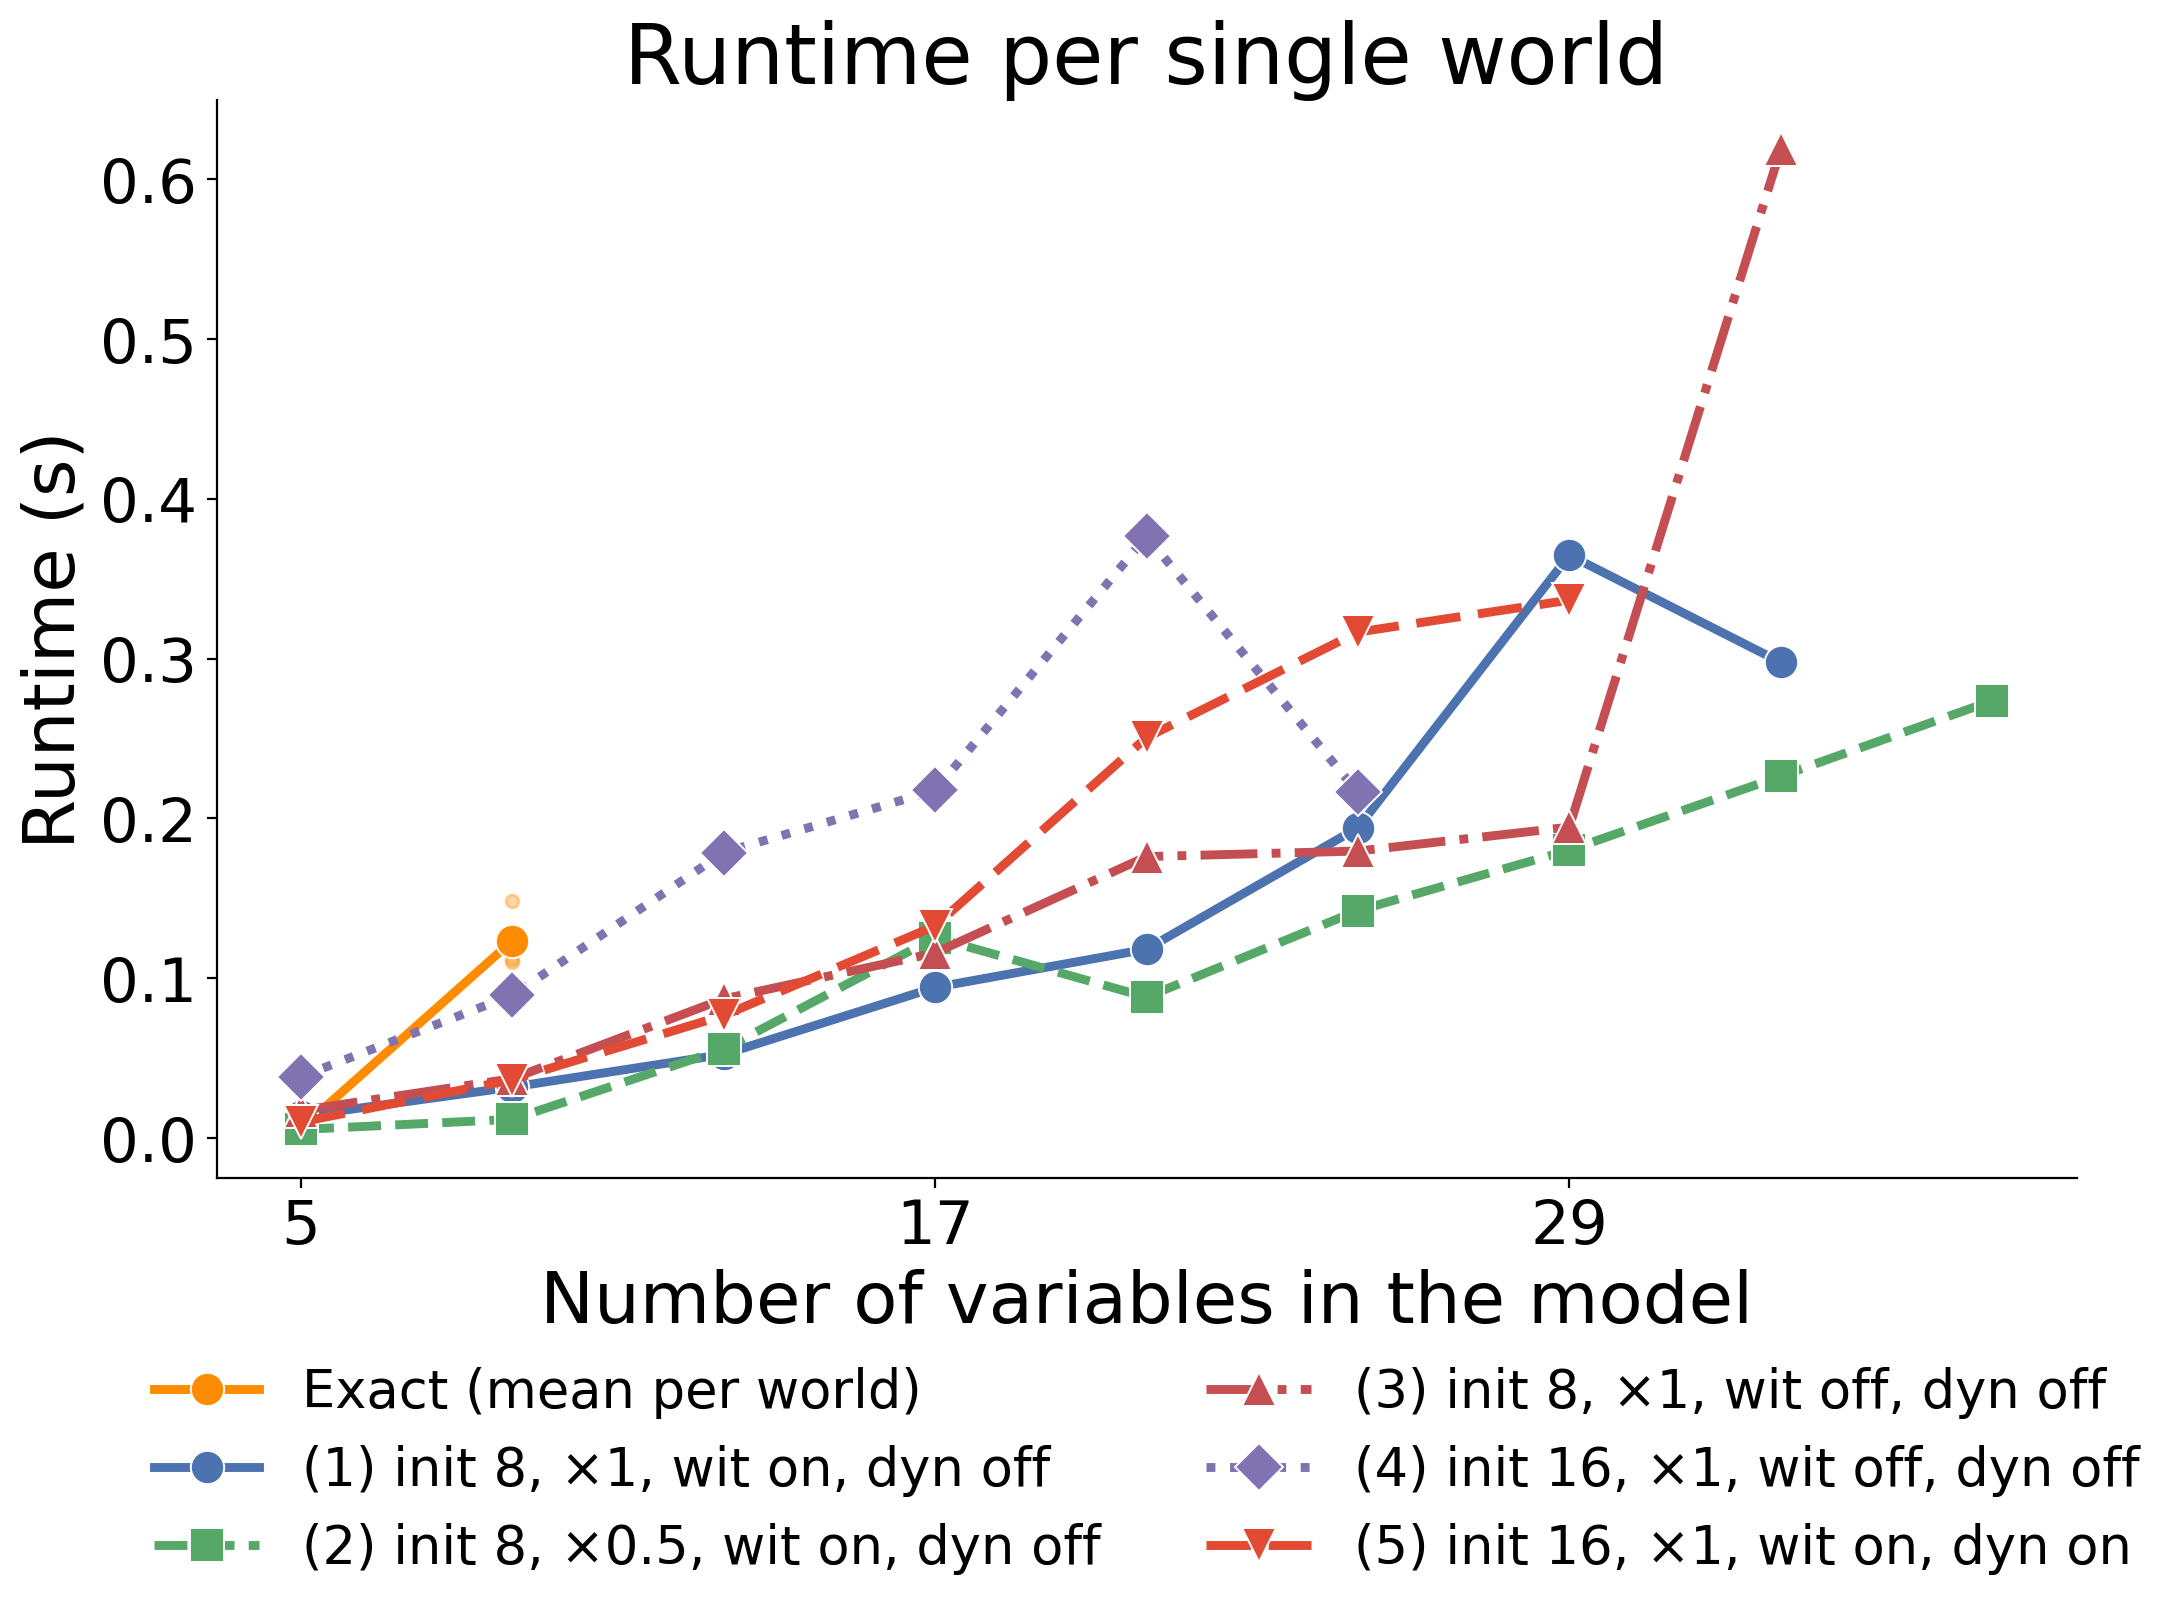
\includegraphics[width=0.92\linewidth]{docs/source/ac_benchmark/plot1_runtime.png}
\caption{Per-world runtime against problem size. The exact method (orange) times
out at 17 variables; approximate methods continue, with reach controlled by total
sample budget. Five approximate configurations vary initial sample size, the
linear-growth factor $\alpha$, the witness ablation, and dynamic cardinality
bounds; see Benchmark protocol.}
\label{fig:ac_runtime}
\end{figure}

\begin{figure}[htbp]
\centering
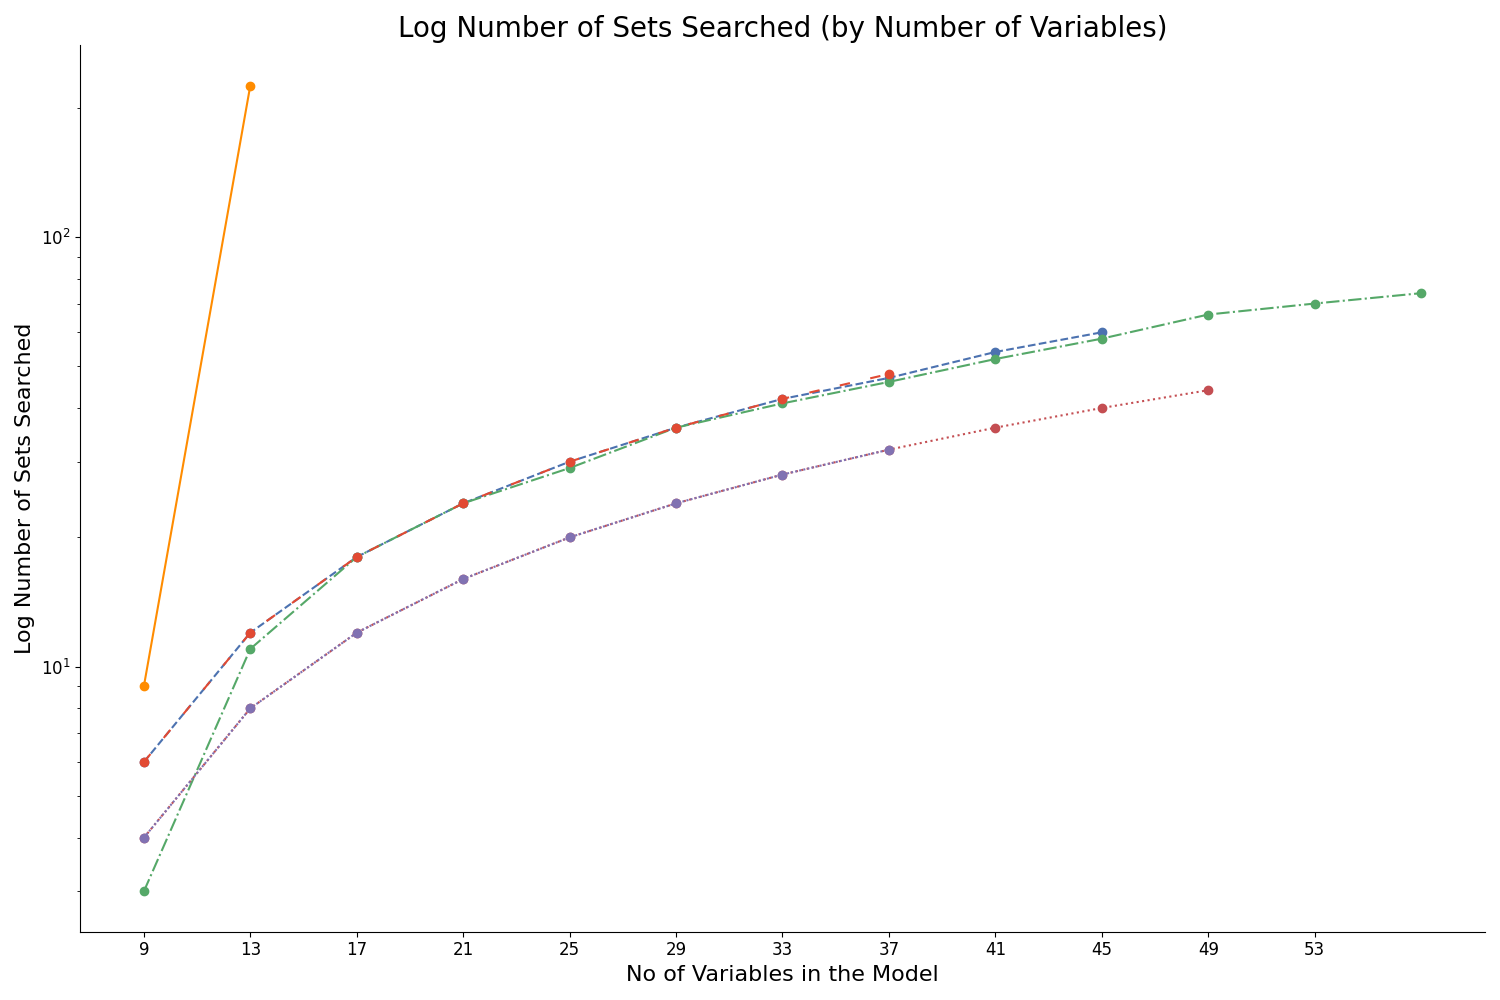
\includegraphics[width=0.92\linewidth]{docs/source/ac_benchmark/plot2_search_space.png}
\caption{Number of cause-witness configurations explored per problem size, log
scale. The exact method visits the full powerset; the approximate methods visit a
few hundred unique configurations per problem size regardless of $n$ --- a gap of
several orders of magnitude that grows with $n$.}
\label{fig:ac_search_space}
\end{figure}

\begin{figure}[htbp]
\centering
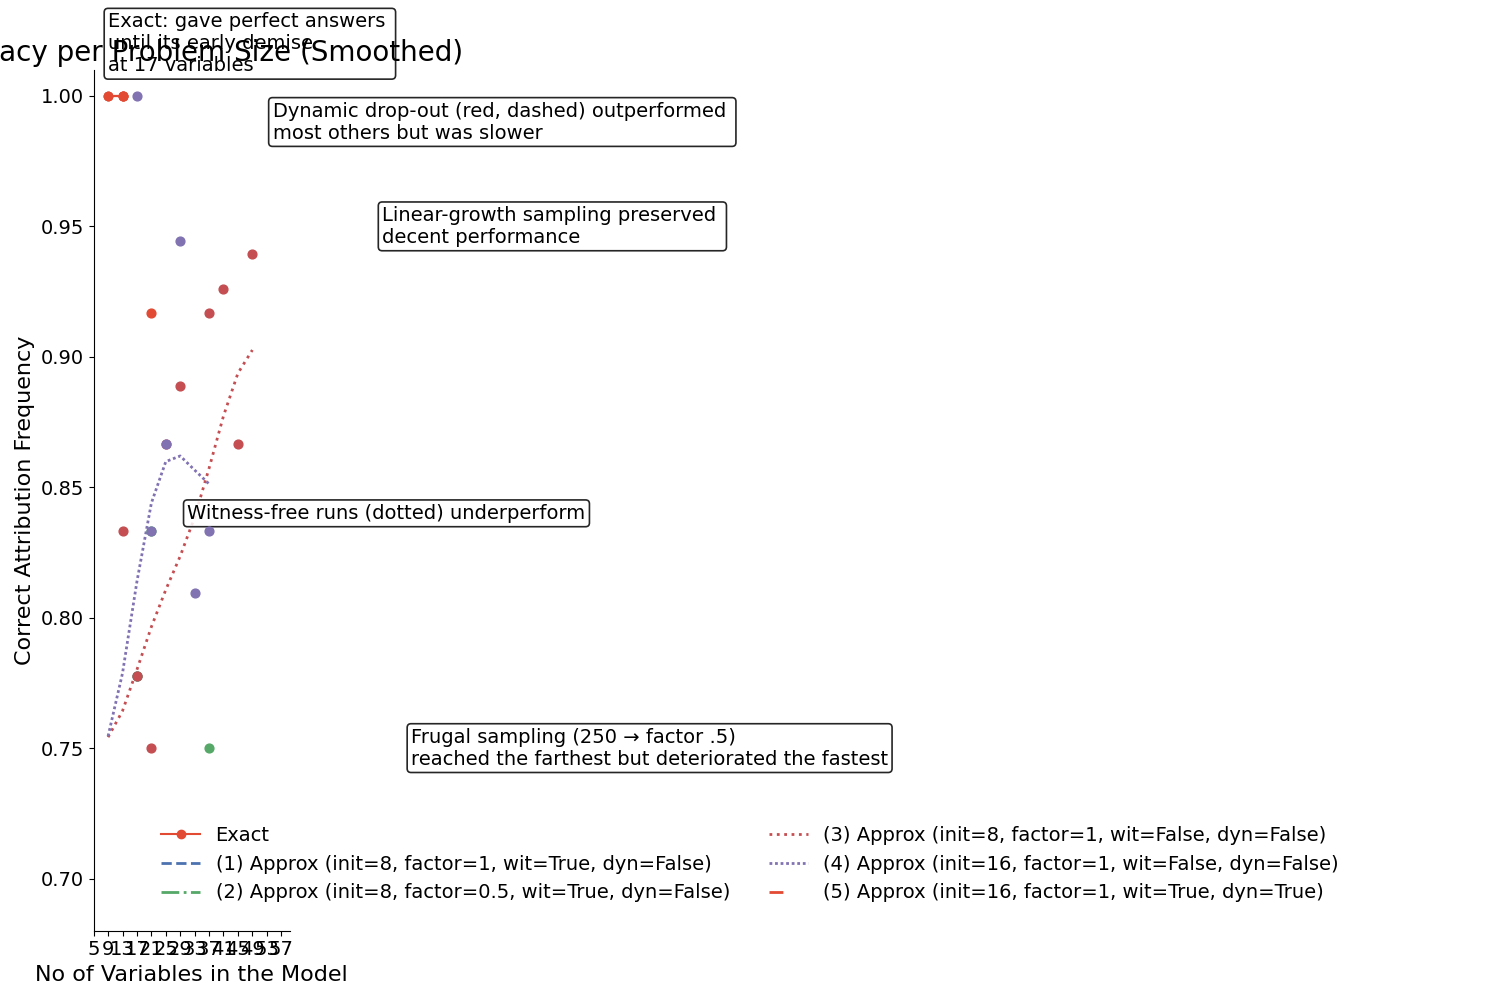
\includegraphics[width=0.92\linewidth]{docs/source/ac_benchmark/plot3_accuracy.png}
\caption{Correct-attribution rate against problem size, smoothed with a Gaussian
filter. The exact method is correct up to 17 variables. Witness-using approximate
runs stay above $0.85$ up to roughly 60 variables and degrade gracefully
thereafter; witness-free runs (dotted) underperform throughout, starting near
$0.67$. Dynamic-set-size sampling (dashed red) is among the highest at moderate
problem sizes.}
\label{fig:ac_accuracy}
\end{figure}

\medskip\noindent\textit{Scope of the conclusion.}
The benchmark establishes that the necessity-only PCI estimator tracks AC verdicts
on a faithful scaling of the canonical example with several orders of magnitude
fewer evaluated configurations. The problem itself, however, is structured:
responsibility attribution is independent across sites, exactly one of $A_i,B_i$ is responsible at
each site given $C{=}1$, supersets of any witness set witness the same attribution
(so a small witness-cardinality bound costs little), and all variables are binary.
These regularities account for some of the favourable scaling --- in particular,
the cardinality-bounded sampling losing little to dynamic-set-sizes sampling on
this problem. Two extensions are natural follow-ups. First, a comparison against
SHAP and causal SHAP on the same scaled-throwing problem is deferred to a
companion benchmark (cf.\ Section~\ref{sub:synthetic} for the corresponding
comparison on the continuous overdetermination example); the sufficiency component
of PCI is what distinguishes it from those baselines, and a clean head-to-head
requires the joint kernel rather than the necessity-only restriction used here.
Second, benchmarks that break each of the structural regularities above ---
particularly continuous-variable extensions where AC's mechanical enumeration is
no longer even well-defined --- would test the estimator outside its current
favourable regime. As a sanity check that the correspondence in
Theorems~\ref{th:ac-exp}--\ref{th:exp-ac} is empirically operational at scale, the
present comparison is sufficient.

\section{Dynamical SIR Benchmark: PCI on Continuous Outcomes}\label{sec:sir_benchmark}

The actual-causality benchmark of Section~\ref{sec:ac_benchmark} exercises the
necessity-only specialisation of \ourapproach on a discrete outcome with a
closed-form ground truth. This section shifts to the regime where AC has no
verdict to compare against: a Bayesian dynamical model with a continuous
outcome and asymmetrically interacting causes. The benchmark mirrors a public
chirho tutorial%
\footnote{\url{https://basisresearch.github.io/chirho/explainable_sir.html}}
in setup and query, which uses chirho's \texttt{SearchForExplanation} handler
to compute classical actual-cause probabilities. We keep the same model and
the same query but replace the explanatory machinery with the \ourapproach
thin-search sampler. The full implementation, raw outputs and plotting code
are in the companion notebook
\texttt{docs/source/sir\_benchmark.ipynb}.

\medskip\noindent\textit{Model.}
The dynamics are the standard SIR system
\(\dot S = -\beta S I,\, \dot I = \beta S I - \gamma I,\, \dot R = \gamma I\),
with Bayesian priors $\beta\sim\mathrm{Beta}(18,600)$ and
$\gamma\sim\mathrm{Beta}(1600,1600)$. Two non-pharmaceutical policies, each
enacted with prior probability $1/2$, modulate the transmission rate via an
intervention strength $l\in[0,1]$ that scales $\beta_0$ to $(1-l)\beta_0$.
Lockdown alone has efficiency $0.6$; masking efficiency depends on lockdown
($0.1$ under lockdown, $0.45$ on its own); the joint efficiency is the
clamped sum, capped at $0.95$. Lockdown is enacted at $t=1$, masking at
$t=1.5$. The outcome is the \emph{overshoot}, the peak-to-final $S$ gap
of the simulated trajectory, and the undesirable event is
$\mathrm{os\_too\_high}=\mathbbm{1}[\mathrm{overshoot}>24]$ on a $100$-person
population.

\medskip\noindent\textit{But-for analysis fails to separate the suspects.}
Conditioning on each pair of policy decisions and drawing $100$ predictives
yields $\Pr(\mathrm{overshoot}>24) \approx 0.07$ with no intervention, $0.67$
with both policies, but $0.82$ with lockdown only and $0.87$ with mask only.
The mechanism is the asymmetric joint efficiency: combining the two policies
caps the transmission reduction at $0.95$, but neither policy alone reaches
that cap, and mask-only is comparatively weak unless lockdown is absent (which
shifts mask efficiency from $0.1$ to $0.45$). But-for cannot disentangle this
context dependence: it treats each policy as a binary cause and reports an
aggregate effect, with no way to express that lockdown's causal contribution
depends on whether masking is in force. Figure~\ref{fig:sir_trajectories}
visualises the four interventional regimes: the trajectory bands collapse
toward the unintervened baseline only under both policies, while either
policy on its own leaves the infectious peak essentially intact, mirroring
the near-equal but-for overshoot probabilities.

\begin{figure}[htbp]
\centering
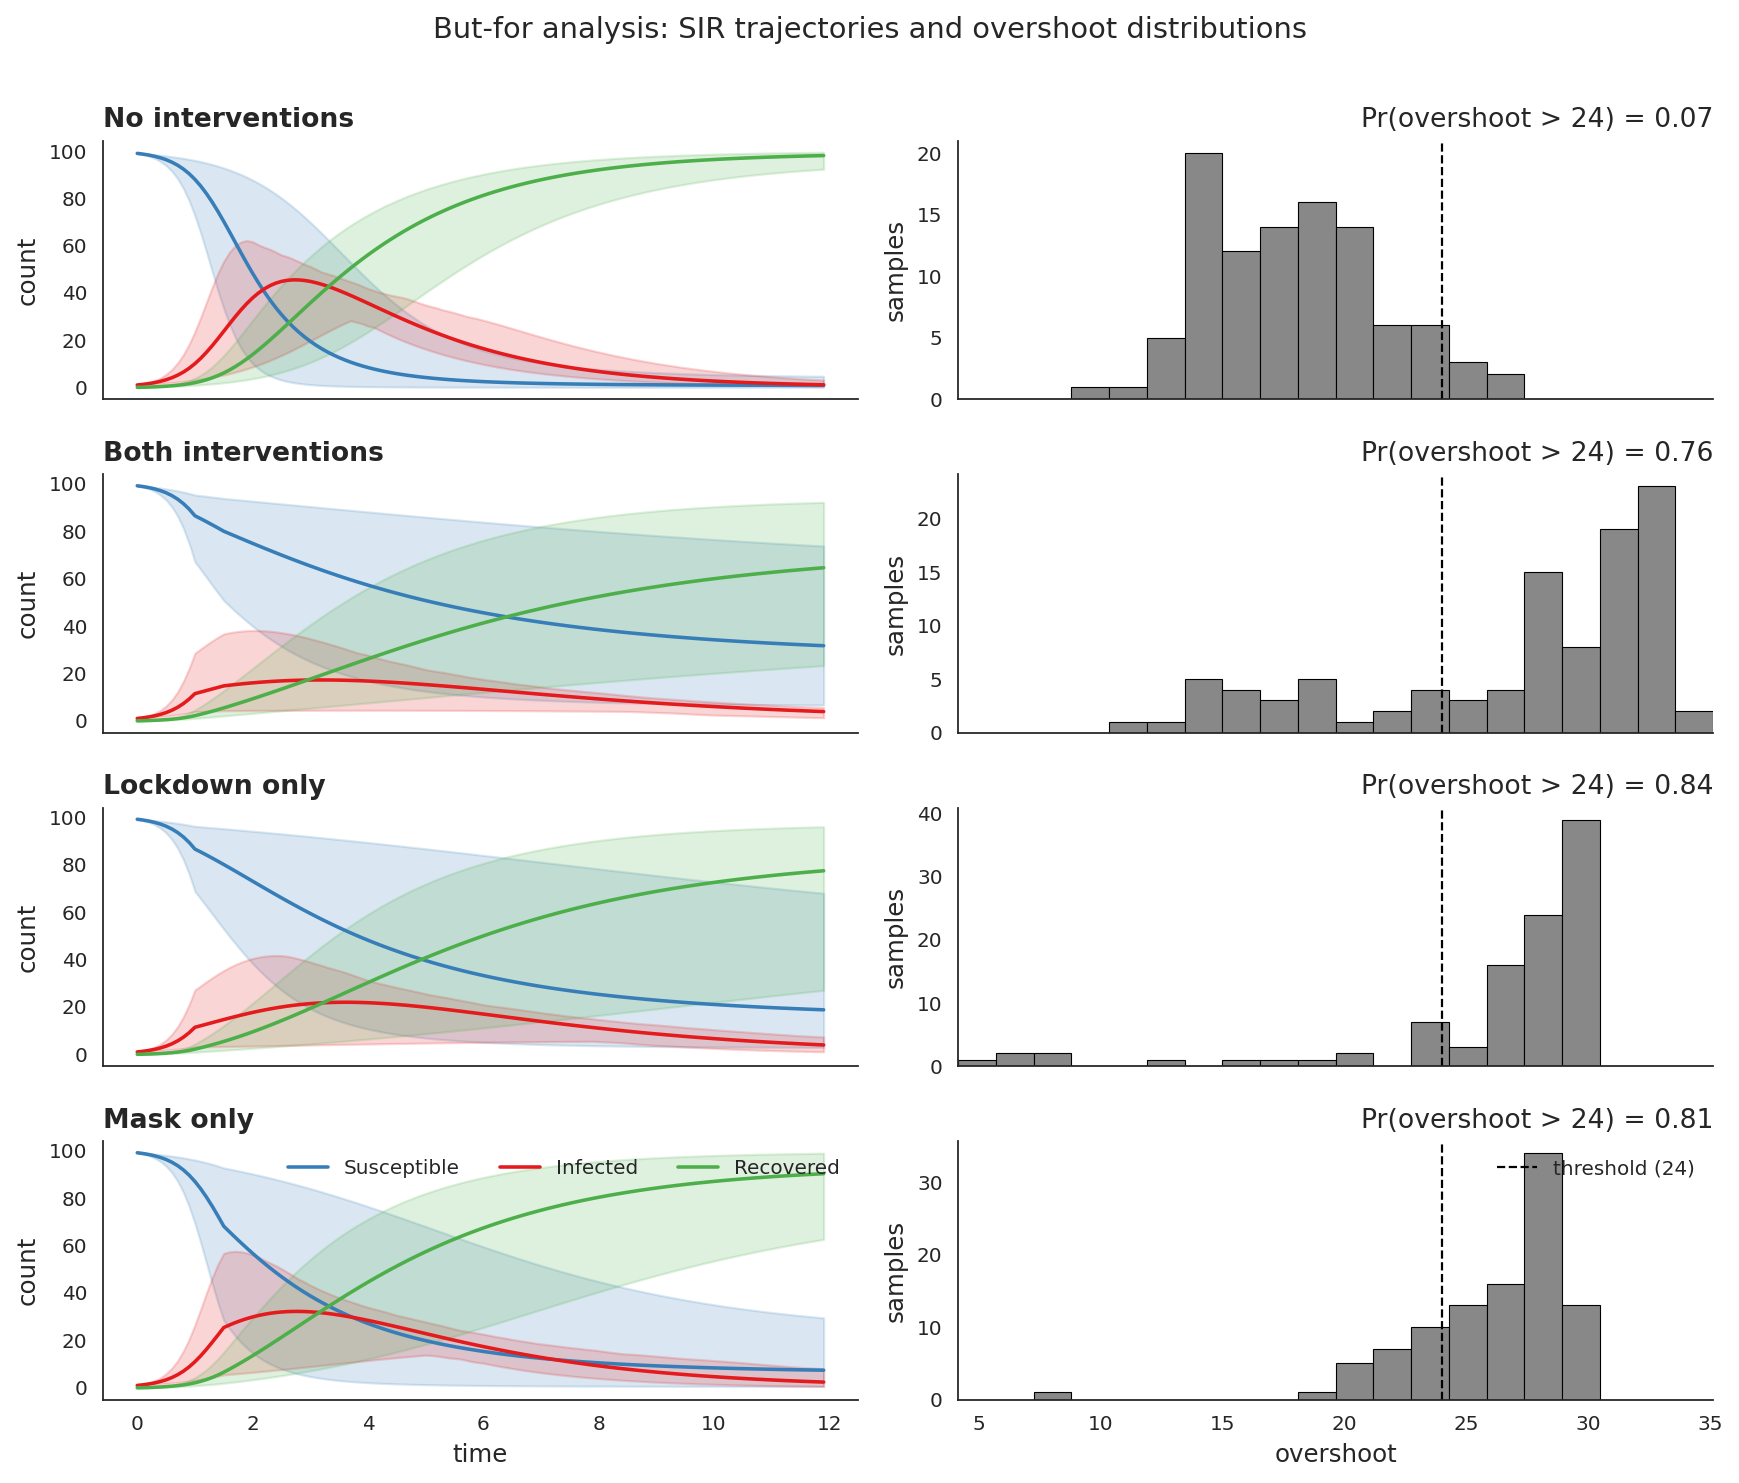
\includegraphics[width=0.92\linewidth]{docs/source/sir_benchmark/sir_butfor.png}
\caption{SIR trajectories and overshoot distributions under the four
interventional regimes (no interventions, both policies, lockdown only, mask
only). Left: posterior bands for susceptible (blue), infectious (red) and
recovered (green) over time, with the lockdown enacted at $t=1$ and the mask
mandate at $t=1.5$. Right: per-regime histograms of the overshoot, with the
$24$-overshoot threshold marked. Either policy on its own leaves the
infectious peak essentially intact; only the joint regime suppresses it
appreciably, yet the lockdown-only and mask-only overshoot probabilities are
near-indistinguishable: the asymmetric joint efficiency that
\ourapproach disentangles.}
\label{fig:sir_trajectories}
\end{figure}

\medskip\noindent\textit{\ourapproach thin-search procedure.}
The suspects are $\{\mathrm{lockdown},\mathrm{mask}\}$. The witnesses are
drawn from the policy efficiencies
$\{\mathrm{lockdown\_efficiency}, \mathrm{mask\_efficiency},
\mathrm{joint\_efficiency}\}$, with the suspect itself excluded from the
witness set on each draw. The factual world fixes both policies on
($\mathrm{lockdown}=1, \mathrm{mask}=1$), so the factual outcome
$y^\star=\mathrm{overshoot}$ is read from the same trajectory. For each
suspect the sampler draws $2{,}500$ regimes, scoring each with the
$|y^\star-y_{\mathrm{nec}}| - |y^\star-y_{\mathrm{suff}}|$ statistic and
averaging across regimes. The $\mathrm{nec}$ term rewards regimes where
removing the suspect moves the outcome \emph{away} from $y^\star$; the
$\mathrm{suff}$ term rewards regimes where fixing the suspect at factual
keeps the outcome \emph{close} to $y^\star$.

\medskip\noindent\textit{Single-world results.}
\ourapproach assigns lockdown roughly $2.0\times$ the responsibility of
mask:
\begin{center}
\small
\begin{tabular}{lccc}
\toprule
suspect & $\overline{|y^\star\!-\!y_{\mathrm{nec}}|}$ &
          $-\overline{|y^\star\!-\!y_{\mathrm{suff}}|}$ &
          total \\
\midrule
lockdown & $8.12$ & $-6.58$ & $\mathbf{1.54}$ \\
mask     & $7.43$ & $-6.67$ & $\mathbf{0.76}$ \\
\bottomrule
\end{tabular}
\end{center}
The gap is driven entirely by the necessity term: removing lockdown moves
the overshoot further from $y^\star$ than removing mask does ($8.12$ vs
$7.43$ in mean absolute distance), while the sufficiency terms agree to
within $0.1$. This is consistent with the but-for finding that either
policy \emph{alone} is roughly equally bad. What distinguishes the suspects
is that lockdown's removal \emph{under context} (with witnesses pinned to
factual) pulls the world further from $y^\star$ than mask's removal does.
Figure~\ref{fig:sir_heatmap} makes the necessity-term gap visible. Each
point is one sampled regime, with $y_{\mathrm{nec}}$ on the horizontal axis
(focal suspect intervened to alternative, other active suspects in
$\mathbf{C}\setminus\{X\}$ intervened, witnesses at factual) and
$y_{\mathrm{suff}}$ on the vertical axis (focal suspect at factual, other
active suspects intervened, witnesses at factual). The dotted red cross-hair
marks the factual outcome $y^\star$ at the both-policies-on world
($\mathrm{lockdown}=\mathrm{mask}=1$); because that world is the
high-overshoot scenario, $y^\star$ sits near the upper-right of the cloud
rather than at its centre, and a regime contributes positively to the score
iff its point lies further from the cross-hair along $x$ than along $y$.
Under that geometry the lockdown density is shifted noticeably toward
smaller $y_{\mathrm{nec}}$ at fixed $y_{\mathrm{suff}}$ --- removing
lockdown pulls $y_{\mathrm{nec}}$ well below $y^\star$ while
sufficiency-side overshoot stays close to $y^\star$ --- whereas the mask
density sits closer to the $y_{\mathrm{nec}}=y_{\mathrm{suff}}$ diagonal,
indicating that removing mask does not pull the world as far from
$y^\star$.

\begin{figure}[htbp]
\centering
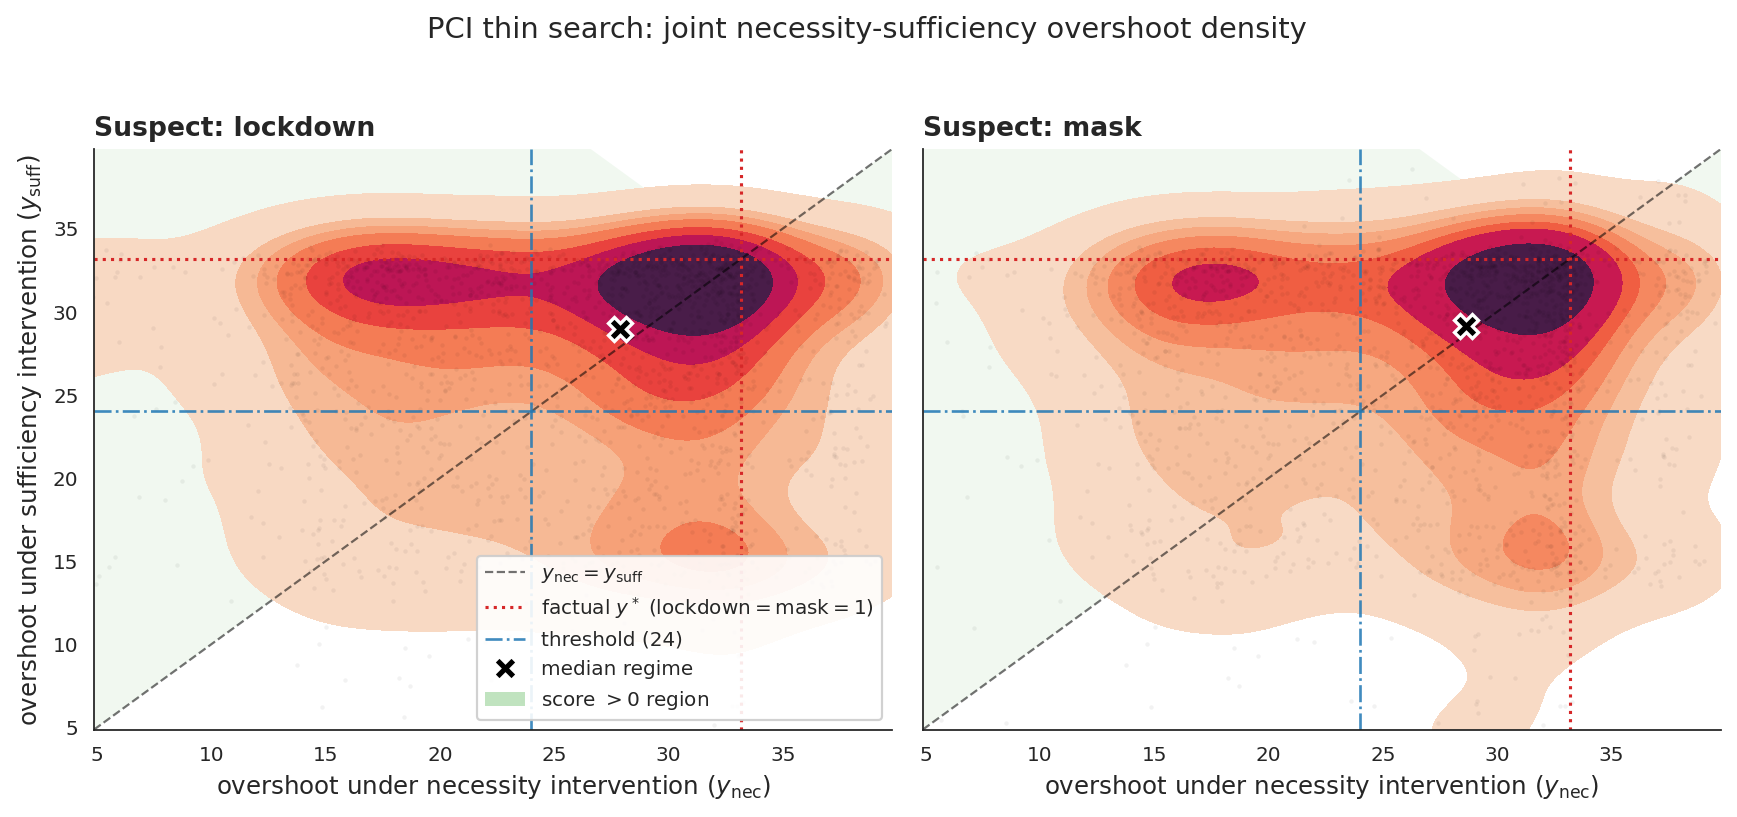
\includegraphics[width=0.92\linewidth]{docs/source/sir_benchmark/sir_heatmap.png}
\caption{Joint necessity-sufficiency overshoot density per suspect. Each
point is one sampled regime. Dotted red cross-hair: factual $y^\star$ at
$\mathrm{lockdown}=\mathrm{mask}=1$ (the high-overshoot anchor); dash-dot
blue: the $24$-overshoot threshold; dashed black:
$y_{\mathrm{nec}}=y_{\mathrm{suff}}$. A regime contributes positively to
the PCI total iff it sits further from the red cross-hair along the
necessity axis than along the sufficiency axis. The lockdown density is
shifted toward smaller $y_{\mathrm{nec}}$ relative to $y_{\mathrm{suff}}$
(the cause signature on this geometry); the mask density sits closer to
the diagonal.}
\label{fig:sir_heatmap}
\end{figure}

\medskip\noindent\textit{Robustness across factual worlds.}
We replicate the analysis across $10$ factual worlds drawn from the prior
(rather than the single hand-set world above), running thin search on each
and averaging. Lockdown's mean total exceeds mask's in the majority of
worlds; the verdict is not an artifact of the chosen factual.

\medskip\noindent\textit{Effect of context.}
The chirho tutorial isolates one downstream variable at a time, asking
whether the verdict survives when that variable is held fixed at factual
versus left free. We replicate the experiment by partitioning the
\ourapproach regimes by whether the partner-policy efficiency variable was
sampled into the witness set
(Figure~\ref{fig:sir_contexts}). For lockdown, with
$\mathrm{mask\_efficiency}$ \emph{fixed} as a witness the score is $0.81$;
\emph{free}, it rises to $2.67$. For mask, with $\mathrm{lockdown\_efficiency}$
\emph{fixed} the score is $-0.48$ (mask fails to register as a cause at
all under that context regime) and \emph{free} it rises to $2.72$.
Lockdown therefore registers as a cause in both context regimes, while
mask's status as a cause is contingent on its partner being allowed to
adapt. \ourapproach thus expresses not just \emph{which} policy is the
dominant cause but \emph{how robustly} that causal claim holds across
counterfactual contexts: a finer-grained verdict than the binary
``actual cause / not'' that classical AC produces.

\begin{figure}[htbp]
\centering
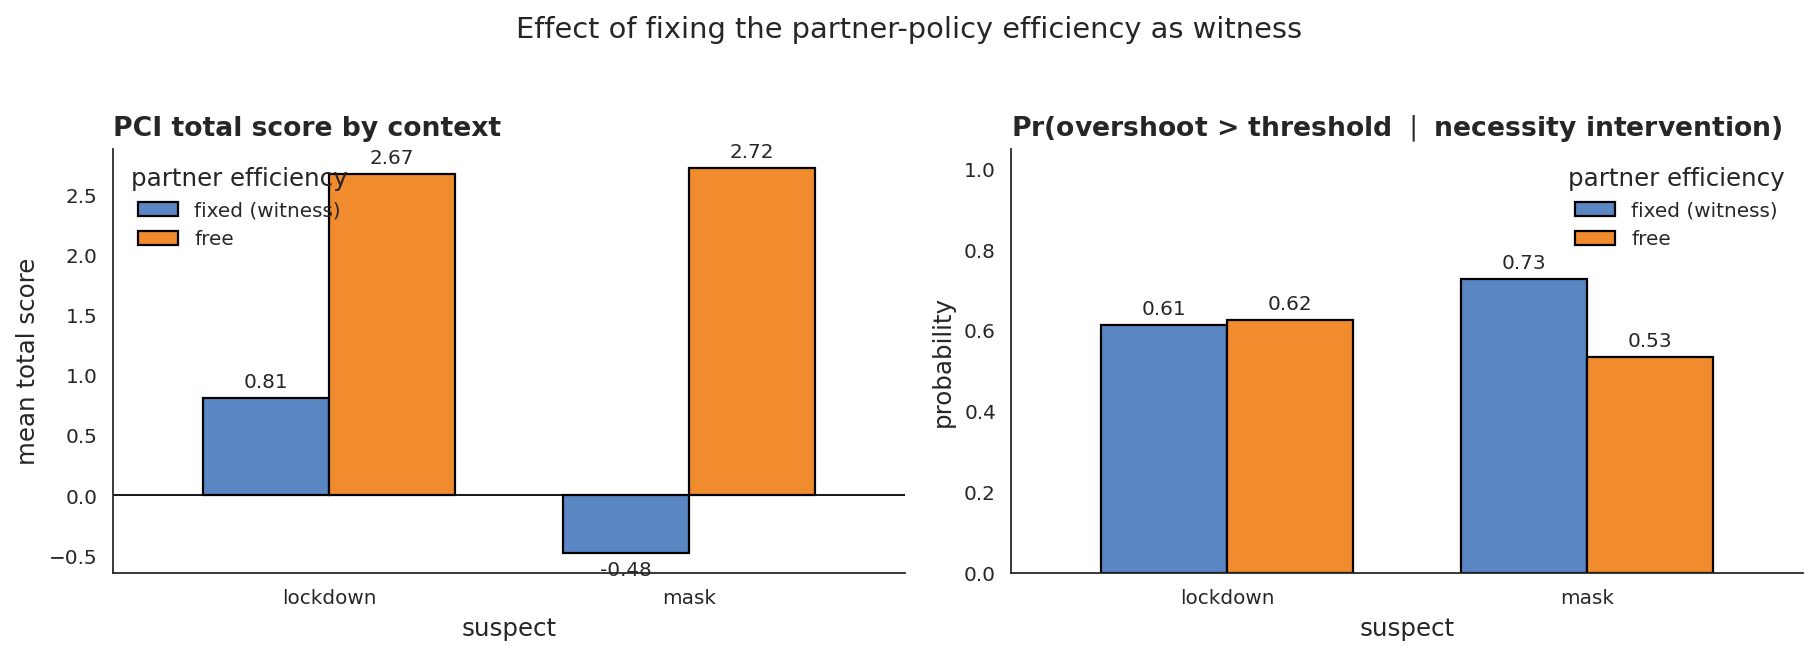
\includegraphics[width=0.92\linewidth]{docs/source/sir_benchmark/sir_contexts.png}
\caption{Different-contexts experiment. Bars compare PCI total score (left)
and $\Pr(\mathrm{overshoot}>24\mid\mathrm{necessity})$ (right) when the
partner-policy efficiency variable is fixed as a witness versus left free.
Lockdown's score is positive in both regimes; mask's score flips sign
across regimes, indicating that mask is a context-sensitive rather than a
robust cause.}
\label{fig:sir_contexts}
\end{figure}

\medskip\noindent\textit{Takeaway.}
On the dynamical SIR setting, \ourapproach recovers the qualitative
diagnosis of the chirho tutorial --- lockdown is the proximate cause of
excessive overshoot, despite both policies appearing similar under but-for
analysis --- and expresses it on a continuous, decomposable scale. The
necessity-vs-sufficiency decomposition distinguishes suspects whose
isolation effects are similar but whose removal-under-context effects
diverge; the contexts experiment further distinguishes robust from
context-sensitive causes. The same machinery applies to any chirho
probabilistic program with a continuous outcome and a tractable enumeration
over interventional regimes.

\paragraph{Where we go next.} The SIR benchmark scales \ourapproach to a
research-grade Bayesian dynamical model and demonstrates that the joint kernel
captures patterns that AC cannot adjudicate. Section~\ref{sec:avm} pushes the
demonstration one step further: a deployed automated valuation model trained on
millions of points, with deep neural-network components and a sparse variational
GP outcome head. The question there is no longer whether \ourapproach agrees with
a known ground truth (on a proprietary production model none is available),
but whether the computation is feasible at all, and whether the qualitative
SHAP-vs-PCI divergences observed on the synthetic side persist on a real trained
system.

\section{Scaling \ourapproach to a Real-World Automated Valuation Model}\label{sec:avm}

 This appendix details the deployed-AVM study summarised in \cref{sec:evaluation}.

The synthetic archetypes of \cref{sub:synthetic}, the AC benchmark of
\cref{sec:ac_benchmark}, and the SIR benchmark of \cref{sec:sir_benchmark} all
controlled the model and the ground truth, so that \ourapproach could be judged
against an analytic verdict or a competing AC enumeration. Here we drop both,
applying \ourapproach to a deployed valuation model for residential housing on
which neither ground truth nor exact AC enumeration is available. Disclosure
constraints on the trained model and its training data prevent a quantitative
accuracy comparison on this system, so the quantitative validation of
\ourapproach{} lives entirely in the controlled synthetic benchmark of
\cref{sub:synthetic}. The role of this appendix is correspondingly narrow: to
report (i) that \ourapproach{} is computationally feasible at production scale on a
model with millions of training points, and (ii) that the qualitative SHAP-vs-PCI
divergence observed in \cref{sec:shap_examples} persists when the model is a real
trained one: the shape of the two attribution distributions and where
attribution mass lands, not the substantive content of the features they assign to.

\paragraph{Setting.}
The unit of analysis is a residential property transaction. \ourapproach is run
against the full country-level production AVM; what we show here is an
illustrative prototype based on the state of New York rather than
the full national model structure, which we cannot disclose in detail. The NY
prototype shares the architecture and the causal-kernel construction described
below with the full system but is smaller in scope and DAG complexity. The
computational-feasibility claim refers to the full national system; the
qualitative SHAP-vs-PCI behaviour we illustrate is a property of the shared
architecture and carries over from the prototype. The
outcome variable $y$ is the (log-epsilon-standardized) sale price. Transactions are
described by a set of categorical variables $x_{cat} = x_{1}, \dots, x_k$ and continuous
(transformed) variables\footnote{Usually log-epsilon-standardized,
standardized-truncated, or standardized.} $x_{con} = x_{k+1}, \dots, x_n$.

\paragraph{Causal model.}
A causal DAG $\mathcal{G}$ expresses our causal assumptions about the relationships between
variables. We wrote it manually in collaboration with domain experts, then refined it by
adding edges to break implied conditional independencies not upheld by the
data. The simplified NY-prototype DAG has 25 nodes and 99 edges; topology with anonymised node
labels is shown in Figure~\ref{fig:avm_dag}; the full national DAG is larger and is
not shown. As demonstrated in \cref{sec:ac_benchmark}, even the prototype is
already large enough that exact actual-causality enumeration is computationally
infeasible, and the same conclusion applies a fortiori to the national system.

Variables $x_i$ are drawn from distributions $\mathrm{Dist}_i$ parameterized by functions
$f_i(\mathrm{pa}_i, \varphi_i)$ of the parent variables
$\mathrm{pa}_i$\footnote{For root nodes, $\mathrm{pa}_i$ is empty.}:
$x_i \sim \mathrm{Dist}_i(f_i(\mathrm{pa}_i, \varphi_i))$. We call these distributions
\emph{causal kernels}. The distributions are either (truncated) normal or categorical; we choose the
family based on the domain of the variable it models. The functions $f_i$ are deep
neural networks with parameters $\varphi_i$, which we optimize using cross-entropy
loss for categorical distributions and average negative log likelihood for
continuous distributions. The outcome is modeled by a sparse variational
Gaussian Process (SVGP; \citealp{titsias2009variational,hensman2013gaussian}),
$x_{gp} = (x_{con}, \eta(x_{cat}, \varphi_{cat}))$,
$y \sim \mathcal{SVGP}\!\left(\mu(x_{gp}, \varphi_\mu), \kappa(x_{gp}, \varphi_\kappa)\right)$,
where $\eta$ is a linear embedding of the categorical variables into the continuous
space, jointly optimized with the GP.

\begin{figure}[htbp]
\centering
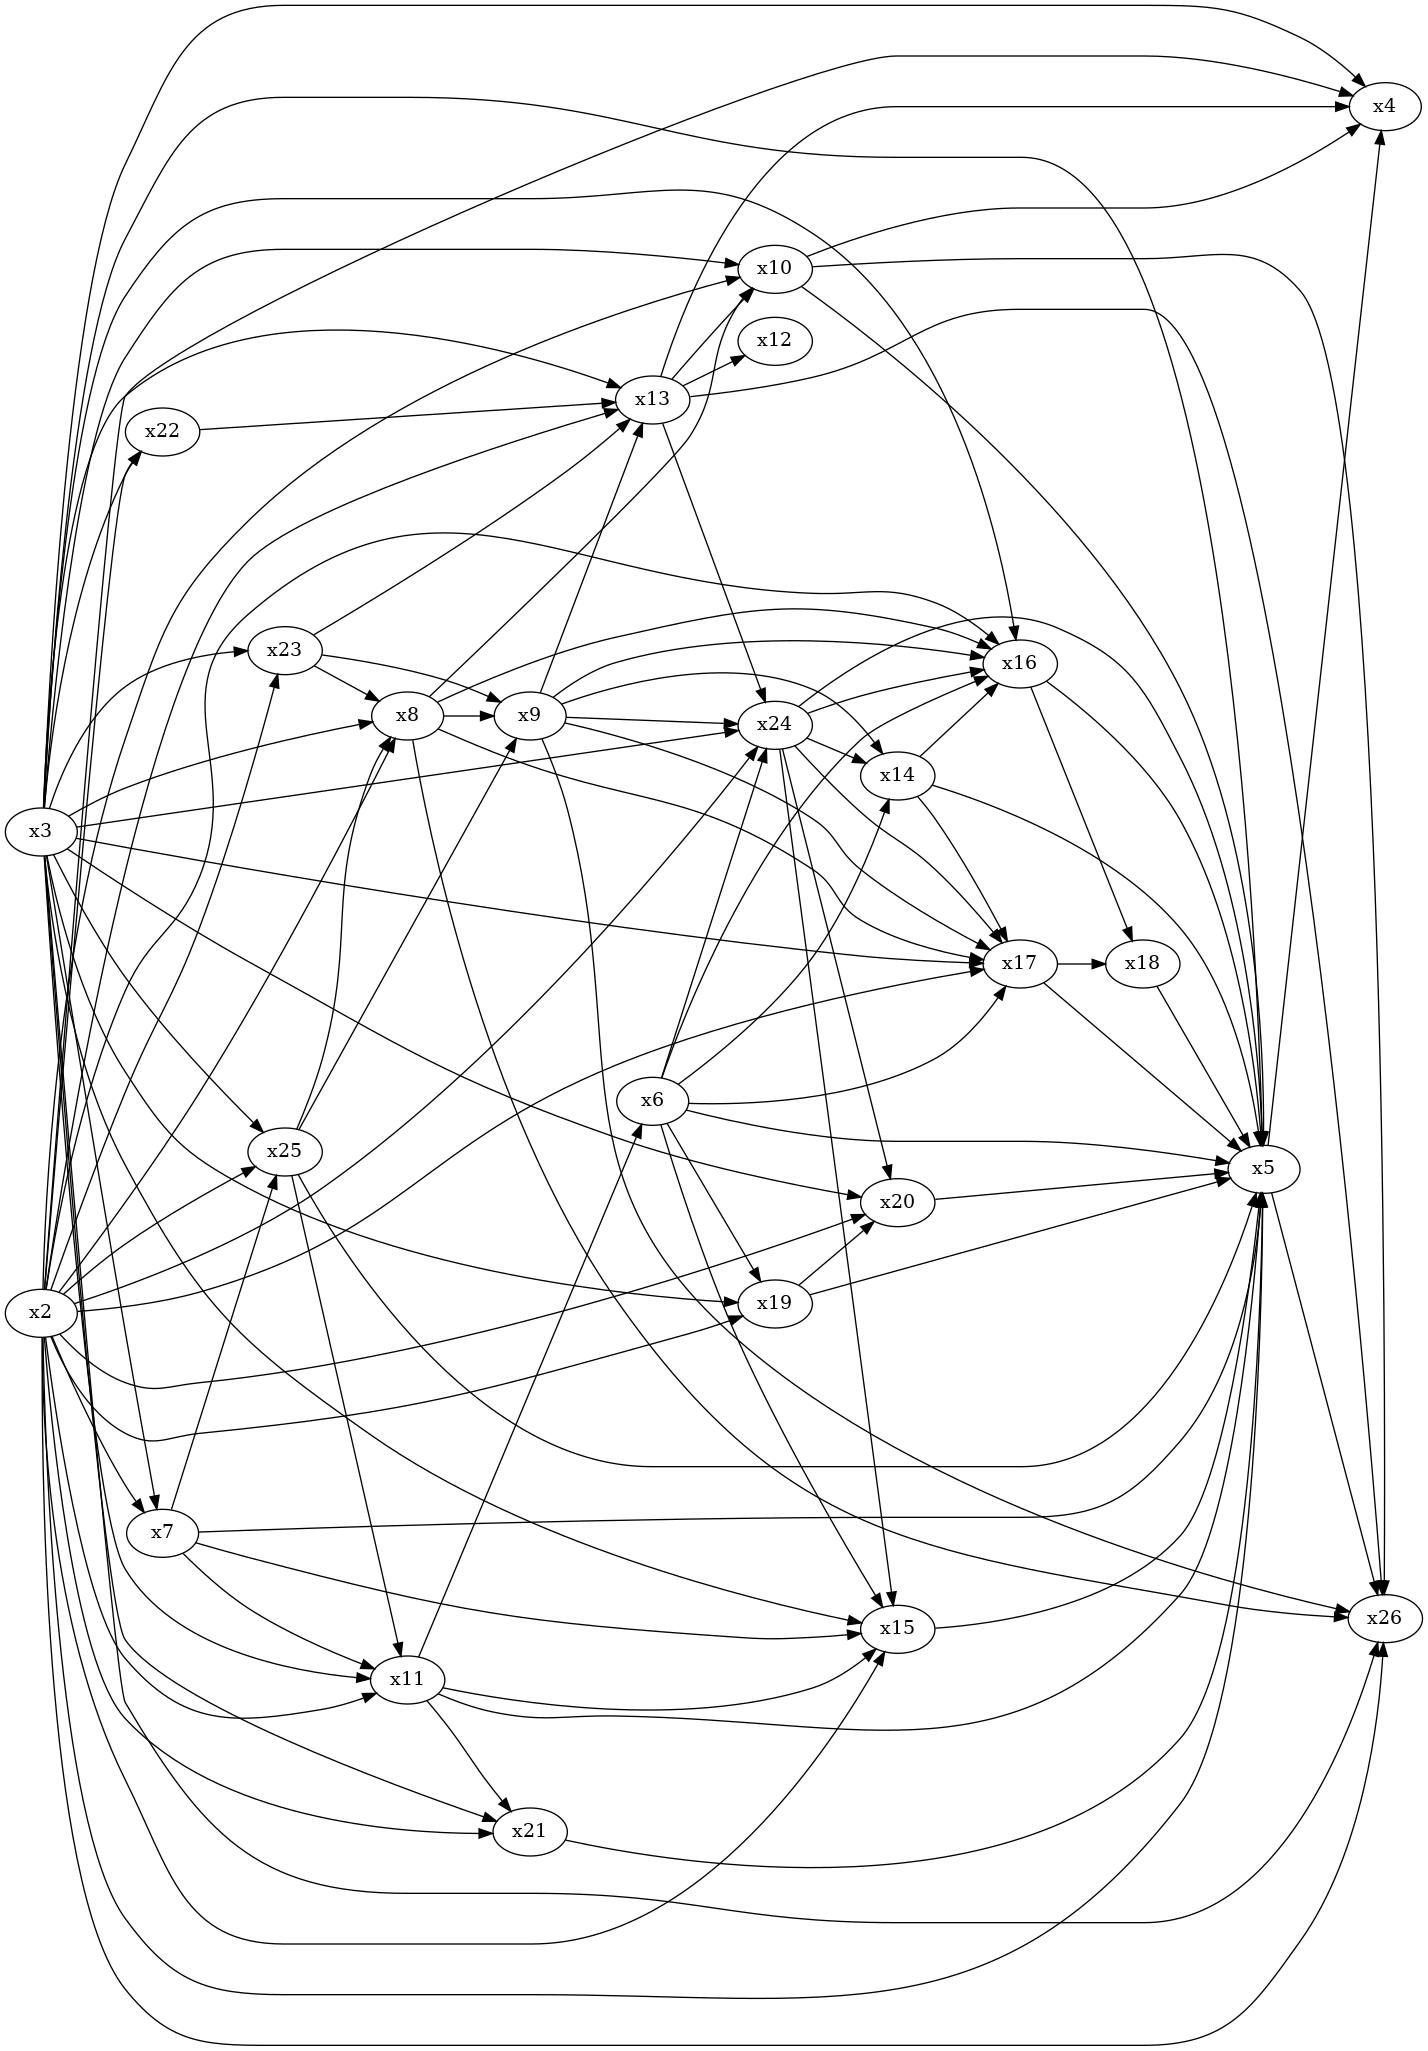
\includegraphics[width=0.85\linewidth]{figures/anonymized_upstream_structure.png}
\caption{Topology of the AVM causal DAG (NY-prototype version), with node labels
anonymised. The graph has 25 nodes and 99 edges; the full national DAG is larger
and is not shown. Several variables sit deep in the DAG with high in-degree; these
are the nodes towards which SHAP allocates disproportionate attribution mass (see
Figure~\ref{fig:eval_avm}).}
\label{fig:avm_dag}
\end{figure}

\paragraph{Feasibility at production scale.}
To apply \ourapproach we transform the model as described in
Section~\ref{sec:causal_impact} and evaluate the impact of features from a list of
potential causal suspects, using the absolute difference impact score of
Example~\ref{ex:absolute_score}. We draw Monte Carlo samples from the expanded model.
Conditioning on a given suspect $X_i$ being active gives us a sample of the scores
corresponding to that feature, which we use to estimate the expected value thereof. The
estimation converges at around \num{25000} samples; for a batch of 50 data points this
takes around 60 minutes on commodity hardware. We need to sample only once; we can then reuse the samples to compute the
attribution score of any suspect. This
establishes that the method is computationally tractable at production scale, not a
foregone conclusion, since the expanded-model construction in
Section~\ref{sec:causal_impact} introduces additional latent dimensions per suspect and
per witness.

\paragraph{Qualitative comparison to SHAP.}
We compare \ourapproach attributions to SHAP scores \citep{lundberg2017unified} on the
same trained model. SHAP heavily weights variables that are downstream of many other
variables in the causal graph, effectively assigning attribution to what amount to
summary statistics of the outcome. \ourapproach distributes attribution more evenly
across the upstream causal structure. The pattern is consistent with what
Section~\ref{sec:shap_examples} establishes on controlled examples: SHAP's observational
marginalisation allocates weight differently from intervention-and-witness-based PCI
scores, and on a deep DAG this difference manifests as concentration on
summary-statistic-like nodes. Figure~\ref{fig:eval_avm} shows the two attribution
distributions with anonymised feature labels; here we can report the shape of
the two distributions, not which features they assign to.



\section{Discussion and Conclusions}
\label{sec:discussion}

We can now state the main differences between \ourapproach and the
two approaches that inspired it, against the background of what the rest of the paper has
shown. The main lesson from the literature on actual causality is that intuitive causal
attribution often requires holding some endogenous variables, members of a ``witness
set'', fixed at their factual values. This ensures context sensitivity by controlling
complicating causal paths. We treat witnesses differently: instead of looking for
a single witness set that reveals a causal relationship, we use a distribution over
witness sets and integrate the causal impact score across them. As in many probabilistic
generalisations, this focuses on whole distributions, and it lets
\ourapproach account for the number of witness sets and the strength of
within-witness-set effects. Moreover, the construction admits off-the-shelf probabilistic
inference in place of worst-case subset enumeration. The relationship between the two
views is now formal where it was once gestural: under matching choices of $\Gamma$ and
$\Delta$, AC verdicts coincide with the support of $\sum_{\mathbf{T}}\Phi$
(Theorems~\ref{th:ac-exp}--\ref{th:exp-ac} and Proposition~\ref{prop:filter}), and the
empirical companion in \cref{sec:ac_benchmark} confirms this at scales where AC
enumeration is intractable.

The main concept borrowed from Pearl's probability of necessity and sufficiency is the
joint distribution over outcomes from two interventional regimes, pushed forward through
a user-chosen causal impact function. The key difference is that we use witness sets to
allow for context-sensitivity and to break symmetries present in otherwise pathological
cases like overdetermination and undercutting. Section~\ref{sec:shap_examples} works
through the binary instantiation in which the necessity and sufficiency components
coincide with PN and PS, and \cref{sub:synthetic} reads the two components apart on
a continuous synthetic model where each is needed to bring out a different causal
archetype.

The further generalisations are mostly bookkeeping in the same spirit. Instead of fixing
a single alternative value for a potential cause, we integrate over a factual-excised
alternative-value distribution; this generalises immediately to continuous variables.
Instead of asking whether a particular set is an actual cause, we sample suspect sets and
gauge a feature's responsibility in terms of its participation in sets with causal
impact. Instead of asking whether the outcome differs, a customisable causal impact
function $ci$ measures the differences across counterfactual worlds, including between
continuous variables. The variable-selection distribution $\Gamma$, the alternative-value
distribution $\Delta$, and the impact function $ci$ become explicit, user-facing
components of the framework, no longer implicit defaults.

Against SHAP-family attributions, the framework's central commitment is to
\emph{intervention with witnesses} over \emph{observational marginalisation}. The
controlled comparisons of Section~\ref{sec:shap_examples} show that this commitment does
real work on canonical overdetermination and continuous-mediation examples, where SHAP
and Causal SHAP fail in characteristic ways that \ourapproach avoids. The synthetic
benchmark of \cref{sub:synthetic} confirms this on a model with known ground
truth, and the case study of \cref{sec:avm} reports the same qualitative pattern
on a production-grade trained model with millions of data points. A separate comparison
to gradient-based attribution, where the difference is one of differentiability and locality, not the
causal/non-causal axis, is reported in \cref{sec:DCE}. The
thread connecting these results is structural: the witness mechanism that satisfies
D-A-rank for Alice in the binary OBCB walkthrough of
Section~\ref{sec:shap_examples} is the same machinery driving the upstream-versus-downstream
attribution split on the AVM in \cref{sec:avm}.

A broader test is how \ourapproach fares against the desiderata that the XAI
literature typically asks counterfactual-explanation methods to meet, of which
\cite{verma2022recourses} list five. \emph{Sparsity}, the requirement that
explanations change as few features as possible, follows directly from the
cardinality cap on suspect sets in $\Gamma$, which biases the search toward small
$\mathbf{C}$. \emph{Multiple counterfactuals} (the ability to return several
alternative explanations instead of committing to one) falls out of the Monte Carlo
construction, since a single sweep over $\Gamma$ and $\Delta$ produces a population of
$(\mathbf{C}, \mathbf{c}', \mathbf{T})$ triples, not a single optimum.
\emph{Causal-constraint satisfaction}, the demand that explanations respect
downstream propagation rather than treat features as independently editable, is
automatic once suspect interventions are routed through the causal model: changing
$\mathbf{C}$ propagates to descendants by construction. \emph{Model-agnosticism}
(applicability to arbitrary predictors) \ourapproach satisfies only partially: it
can wrap a black-box predictor, but at the cost of the causal sensitivity that
motivates the framework in the first place.

\emph{Actionability}, the requirement that explanations not recommend changes to
features users cannot in practice change, is where we part company with the
literature. The standard recommendation is to fold ease-of-change into the
cause-identification procedure itself, weighting features by mutability so that
immutable ones are never returned as causes (\cite{verma2022recourses}; cf.\
\cite{Karimi2021}, who shift the focus from explanations altogether to interventions).
We think this conflates two distinct questions. A procedure that suppresses gender as
a possible cause whenever a loan decision is at stake will help applicants satisfy the
existing system without surfacing the kind of structural
problem that responsibility attribution can in principle reveal. Cost-of-action
layers can sit downstream of \ourapproach for users who need actionable
recommendations, but they should compose with responsibility attribution instead of
replacing it.

Several limitations are worth flagging. \Ourapproach presumes access to a trained
probabilistic causal model from which counterfactual outcomes can be sampled, a
stronger requirement than methods that work from observational data and a causal graph
alone. The Monte Carlo variance of the estimator grows with model size and with the
cardinalities of suspect and witness sets; \cref{sec:ac_benchmark} reports
empirical scaling and an ablation that isolates the contribution of witness pinning, but
sample-efficient estimators for high-cardinality settings remain an open direction.
Finally, the AVM case study is deliberately limited in disclosure: the apples-to-apples
SHAP-vs-PCI comparison rests on the synthetic benchmark of \cref{sub:synthetic},
with the production model serving as a feasibility witness, not as quantitative
evidence.



In sum, \ourapproach provides a scalable, context-sensitive causal explanation
method for causal probabilistic machine-learning models. A natural probabilistic
generalisation of ideas already in the literature leads to a tractable estimator that can
be paired with standard inference algorithms. We benchmarked the approach against exact
actual-causality computations, characterised its qualitative behaviour on synthetic
models with known ground truth and on canonical SHAP failure cases, and showed its
computational feasibility on a production-grade model.

Prior efforts to mechanise actual-causality reasoning in software --- notably the Actual
Causality Canvas of \citet{ibrahimCanvas2020} and the SAT- and optimization-based
computations of \citet{ibrahimChecking2020}, which operationalise the Halpern--Pearl
definition for forensic investigation, fault diagnosis, and explainable AI --- are built
for \emph{discrete} (typically binary) structural models, where the actual cause is
recovered by combinatorial search over candidate sets. The complementary regime of large,
continuous-valued models has received less attention, and it is there that the exact
notions become harder to apply directly. \Ourapproach develops approximate causal
attribution workable for users of models of non-trivial size, with the design choices left
to the user.


\bibliographystyle{plainnat}
\bibliography{references}

\end{document}
